\documentclass[a4paper, 11pt,notoc]{article}
\pdfoutput=1
\usepackage{jcappub}
\usepackage{graphicx}
\usepackage{booktabs}
\usepackage{verbatim}
\usepackage{caption}
\usepackage{xspace}
\usepackage{hyperref}
\usepackage{multirow}
\usepackage{placeins}
\usepackage{array}
%\usepackage[skip=0cm,list=true,labelfont=it]{subcaption}
\usepackage{subcaption}
%\usepackage[sorting=none,backend=biber]{biblatex}

\usepackage{units}
\usepackage{draftwatermark}
\SetWatermarkText{LHC DM WG DRAFT}
\SetWatermarkLightness{0.9}
\SetWatermarkScale{3.0}
\newcommand{\bra}[1]{\langle #1|}
\newcommand{\ket}[1]{|#1\rangle}
\newcommand{\sigv}{\ensuremath{\langle \sigma v_{\rm{rel}} \rangle}\xspace}
\newcommand{\MET}{\ensuremath{E_T^\mathrm{miss}}\xspace}
\newcommand{\met}{\MET}
\newcommand{\MT}{\ensuremath{M_{T}}\xspace}
%\newcommand{\MET}{\ensuremath{\slashed{E}_T}\xspace}
%\newcommand{\met}{\ensuremath{\slashed{E}_T}\xspace}
\newcommand{\mDM}{\ensuremath{M_{\chi}}\xspace}
\newcommand{\mmed}{\ensuremath{M_{\rm{med}}}\xspace}
\newcommand{\mMed}{\ensuremath{M_{\rm{med}}}\xspace}
\newcommand{\mZ}{\ensuremath{M_{\rm{Z}}}\xspace}
\newcommand{\gDM}{\ensuremath{g_{\rm{DM}}}\xspace}
\newcommand{\gq}{\ensuremath{g_q}\xspace}
\newcommand{\gSM}{\gq}
\newcommand{\gdm}{\gDM}
\newcommand{\ifb}{\ensuremath{\rm{fb}^{-1}}\xspace}
\newcommand{\mA}{\ensuremath{M_{A}}\xspace}
\newcommand{\ma}{\ensuremath{M_{a}}\xspace}
\newcommand{\mH}{\ensuremath{M_{H}}\xspace}
\newcommand{\mHc}{\ensuremath{M_{H^{\pm}}}\xspace}
\newcommand{\sinp}{\ensuremath{\sin\theta}\xspace}
\newcommand{\cosp}{\ensuremath{\cos\theta}\xspace}
\newcommand{\sinbma}{\ensuremath{\sin(\beta - \alpha)}\xspace}
\newcommand{\tanb}{\ensuremath{\tan\beta}\xspace}
\newcommand{\lap}[1]{\lambda_{P#1}} % can use like \lap1 , \lap2
\newcommand{\lam}[1]{\lambda_{#1}} % can use like \lam3
\newcommand{\mh}{\ensuremath{M_{h}}\xspace}
\newcommand{\mt}{\ensuremath{M_{t}}\xspace}
\newcommand{\GamA}{\ensuremath{\Gamma_{A}}\xspace}
\newcommand{\Uli}{\color{red}}
\definecolor{cerulean}{RGB}{44,150,207}
\newcommand{\ATLASComments}{\color{cerulean}}
\newcommand{\dmsimp}{\textsc{DMsimp}\xspace}
\newcommand{\maddm}{\textsc{MadDM}\xspace}
\newcommand{\hdm}{\ensuremath{h+\textrm{DM}}\xspace}
\newcommand{\monoh}{\ensuremath{h+\MET}\xspace}
\newcommand{\monohbb}{\ensuremath{h(bb)+\MET}\xspace}
\newcommand{\monoz}{\ensuremath{Z+\MET}\xspace}
\newcommand{\monozll}{\ensuremath{Z(\ell\ell)+\MET}\xspace}
\newcommand{\monozhad}{\ensuremath{Z(\textrm{had})+\MET}\xspace}
\newcommand{\mg}{\textsc{MadGraph~5}\xspace}
\newcommand{\sens}{\mathcal{S}\xspace}
\newcommand{\senstot}{\mathcal{S}_\textrm{tot}\xspace}
\newcommand{\GeV}{\textrm{GeV}\xspace}
\newcommand{\gev}{\GeV\xspace}
\newcommand{\TeV}{\textrm{TeV}\xspace}
\newcommand{\tev}{\TeV\xspace}
\newcommand{\hdma}{\ensuremath{\textrm{2HDM+a}}\xspace}

\newcommand{\lp}{\ensuremath{l^{+}}\xspace}
\newcommand{\lm}{\ensuremath{l^{-}}\xspace}
\newcommand{\pt}{\ensuremath{p_{T}}\xspace}

\newcommand{\ttbar}{\ensuremath{\bar{t}t}}
\newcommand{\bbbar}{\ensuremath{\bar{b}b}}
%\newcommand*{\TeV}{\ensuremath{\text{Te\kern -0.1em V}}}
%\newcommand*{\GeV}{\ensuremath{\text{Ge\kern -0.1em V}}}
%\newcommand{\pt}{\ensuremath{p_{\mathrm T}}}
%\newcommand{\met}{\ensuremath{E_{\mathrm T}^{\mathrm miss}}}

%\newcommand{\GeV}{{\rm \,GeV}}
%\newcommand{\TeV}{{\rm \,TeV}}
%\newcommand{\MeV}{{\rm \,MeV}}
%\newcommand{\eV}{{\rm \,eV}}
%\newcommand{\cm}{{\rm \,cm}}

\newcommand{\mathsc}[1]{\text{\textsc{#1}}}

\DeclareMathOperator{\arccot}{arccot}

\def\be   {\begin{equation}}   \def\ee   {\end{equation}}
\def\ba   {\begin{array}}      \def\ea   {\end{array}}
\def\bea  {\begin{eqnarray}}   \def\eea  {\end{eqnarray}}
 %\def\bea  {\begin{align}}   \def\eea  {\end{align}}
\def\bean {\begin{eqnarray*}}  \def\eean {\end{eqnarray*}}
 %\def\bea  {\begin{align*}}   \def\eea  {\end{align*}}
\def\nn{\nonumber}

\newcommand{\vev}[1]{\langle {#1} \rangle}

\newcommand{\mgamcnlo}{MG5\_aMC@NLO\xspace}
\newcommand{\A}{A}


\allowdisplaybreaks

%DIF PREAMBLE EXTENSION ADDED BY LATEXDIFF
%DIF UNDERLINE PREAMBLE %DIF PREAMBLE
\RequirePackage[normalem]{ulem} %DIF PREAMBLE
\RequirePackage{color}\definecolor{RED}{rgb}{1,0,0}\definecolor{BLUE}{rgb}{0,0,1} %DIF PREAMBLE
\providecommand{\DIFadd}[1]{{\protect\color{blue}\uwave{#1}}} %DIF PREAMBLE
\providecommand{\DIFdel}[1]{{\protect\color{red}\sout{#1}}}                      %DIF PREAMBLE
%DIF SAFE PREAMBLE %DIF PREAMBLE
\providecommand{\DIFaddbegin}{} %DIF PREAMBLE
\providecommand{\DIFaddend}{} %DIF PREAMBLE
\providecommand{\DIFdelbegin}{} %DIF PREAMBLE
\providecommand{\DIFdelend}{} %DIF PREAMBLE
%DIF FLOATSAFE PREAMBLE %DIF PREAMBLE
\providecommand{\DIFaddFL}[1]{\DIFadd{#1}} %DIF PREAMBLE
\providecommand{\DIFdelFL}[1]{\DIFdel{#1}} %DIF PREAMBLE
\providecommand{\DIFaddbeginFL}{} %DIF PREAMBLE
\providecommand{\DIFaddendFL}{} %DIF PREAMBLE
\providecommand{\DIFdelbeginFL}{} %DIF PREAMBLE
\providecommand{\DIFdelendFL}{} %DIF PREAMBLE
%DIF END PREAMBLE EXTENSION ADDED BY LATEXDIFF


\begin{document}
\title{\begin{boldmath} \huge Dark Matter Working Group recommendation for Two Higgs Doublet Model (draft title) \vspace{7mm} \end{boldmath}}

%%%%%%

\affiliation[*]{DMWG organizers}

%\author[1,]{Andreas~Albert,}
%\affiliation[1]{III. Physikalisches Institut A, RWTH Aachen University, Aachen, Germany}

%\author[2]{Mihailo Backovi\'c,}
%\affiliation[2]{Center for Cosmology, Particle Physics and Phenomenology - CP3, Universite Catholique de Louvain, Louvain-la-neuve, Belgium}

\author[]{Authorlist to be compiled; }

\author[3,*]{Antonio~Boveia,}
\affiliation[3]{Ohio State University, 191 W. Woodruff Avenue
Columbus, OH 43210}
\emailAdd{antonio.boveia@cern.ch}

%\author[4,*]{Oliver~Buchmueller,}
%\affiliation[4]{High Energy Physics Group, Blackett Laboratory, Imperial College, Prince Consort Road, London, SW7 2AZ, United Kingdom}
%\emailAdd{oliver.buchmueller@cern.ch}

%\author[5,*]{Giorgio Busoni,} 
%\affiliation[5]{ARC Centre of Excellence for Particle Physics at the Terascale, School of Physics, University of Melbourne, 3010, Australia}

%\author[6,7]{Albert De~Roeck,}
%\affiliation[6]{Antwerp University, BÐ2610 Wilrijk, Belgium. }
%\affiliation[7]{CERN, EP Department, CH-1211 Geneva 23, Switzerland}

\author[8,*]{Caterina~Doglioni,}
\affiliation[8]{Fysiska institutionen, Lunds universitet, Lund, Sweden}
\emailAdd{caterina.doglioni@cern.ch}



%\author[9,*]{Tristan~DuPree,}
%\affiliation[9]{Nikhef, Science Park 105, NL-1098 XG Amsterdam, The Netherlands}


%\author[10,*]{Malcolm Fairbairn,}
%\affiliation[10]{Physics, King's College London, Strand, London, WC2R 2LS, UK}

%\author[11]{\\ Marie-Helene Genest,}
%\affiliation[11]{Laboratoire de Physique Subatomique et de Cosmologie, Université Grenoble-Alpes, \\ CNRS/IN2P3, 53 rue des Martyrs, 38026 Grenoble Cedex, France}

%\author[12]{Stefania Gori,}
%\affiliation[12]{Department of Physics, University of Cincinnati, Cincinnati, Ohio 45221, USA}

%\author[13]{Giuliano~Gustavino,}
%\affiliation[13]{Universita' di Roma Sapienza, Piazza Aldo Moro, 2, 00185 Roma, Italy e INFN}

\author[14,*]{Kristian~Hahn,}
\affiliation[14]{Department of Physics and Astronomy, Northwestern University, Evanston, Illinois 60208, USA}
\emailAdd{kristian.hahn@cern.ch}

\author[15,16,*]{Ulrich~Haisch,}
\affiliation[15]{Rudolf Peierls Centre for Theoretical Physics, University of Oxford, Oxford, OX1 3PN, United Kingdom}
\affiliation[16]{CERN, TH Department, CH-1211 Geneva 23, Switzerland}
\emailAdd{ulrich.haisch@physics.ox.ac.uk}


%Contributors to be added
%\author{Nicole F.\ Bell,}
%\author{Giorgio Busoni and}
%\author{Isaac W. Sanderson}
%\affiliation{ARC Centre of Excellence for Particle Physics at the Terascale \\
%School of Physics, The University of Melbourne, Victoria 3010, Australia}
%\emailAdd{\tt n.bell@unimelb.edu.au}
%\emailAdd{\tt giorgio.busoni@unimelb.edu.au}
%\emailAdd{\tt isanderson@student.unimelb.edu.au}
%\author[18]{Valerio~Ippolito,} 
%\affiliation[18]{Laboratory for Particle Physics and Cosmology, Harvard University, USA}
%\author[21]{Greg Landsberg,}
%\affiliation[21]{Brown University, Dept. of Physics, 182 Hope St, Providence, RI 02912, USA.}



%\author[7]{Philip~C.~Harris,} 

%\author[17]{Dan~Hayden,}
%\affiliation[17]{Michigan State University, 220 Trowbridge Rd, East Lansing, MI 48824,
%USA}


%\author[8]{Isabelle~John,}

%\author[19,*]{Felix~Kahlhoefer,}
%\affiliation[19]{DESY, Notkestra\ss e 85, D-22607 Hamburg, Germany}

%\author[20]{Suchita~Kulkarni,}
%\affiliation[20]{Institut f\"ur Hochenergiephysik, \"Osterreichische Akademie der Wissenschaften, \\ Nikolsdorfer Gasse 18, 1050 Wien, Austria}


\author[22]{Steven Lowette,}
\affiliation[22]{Physics Department, Vrije Universieit Brussel, Brussels, Belgium}

%\author[11]{Kentarou~Mawatari,}

%\author[23]{Antonio Riotto,}
%\affiliation[23]{Departement de Physique Theorique (DPT) Geneva Cosmology and Astroparticle Group and Centre for Astroparticle Physics  (CAP), 24 quai Ernest Ansermet
%CH-1211 Geneve}

%\author[24]{William~Shepherd,}
%\affiliation[24]{Institut f\"ur Physik, Johannes-Gutenberg-Universit\"at Mainz, Staudingerweg 7, D-55128 Mainz, Germany}

\author[25,*]{Tim~M.P.~Tait,}
\affiliation[25]{Department of Physics and Astronomy, University of California, Irvine, California 92697, USA}
\emailAdd{ttait@uci.edu}

%\author[3]{Emma Tolley,}

%\author[10,*]{\\ Patrick Tunney,}

%\author[26,*]{Bryan~Zaldivar,}
%\affiliation[26]{Laboratoire de Physique Theorique d'Annecy-le-Vieux (LAPTH) 9 Chemin de Bellevue, B.P. 110, F-74941 Annecy-le-Vieux, CEDEX, France}

%\author[24]{Markus~Zinser}

%\author[8,*]{Priscilla~Pani,}
%\affiliation[8]{CERN, PH Department, CH-1211 Geneva 23, Switzerland}

%\author[25,*]{Johanna~Gramling,}
%\affiliation[25]{Department of Physics and Astronomy, University of California, Irvine, California 92697, USA}



\hfill CERN-LPCC-2017-XX


\abstract{
Draft abstract.}
\maketitle


%%%%%%%%%%%%%%%%
\section{Introduction}
\paragraph{Reasoning behind this effort}

\begin{itemize}
\item Simplified models only one signature at a time, sometimes not
gauge invariant
\item One step beyond this: less-simplified models

\item Compare and confront different search sensitivity

\item Combinations among different signatures

\item Find new kinematic regimes / improve searches by exploring
different signatures

\item Still keeping the choice of model generic enough that this is reusable
for theorists

\end{itemize}

\paragraph{Reasoning behind this effort}

\begin{itemize}

\item Reasoning behind the choice of model

\item Highlights more than one signature at a time, depending on
parameters

\item Leaves room for new unexplored kinematic signatures within
existing searches (left for future work)

\item Complete enough, still simplified so that one can choose grid
planes

\item Existing theory effort (HXSWG)
\end{itemize}

We investigate in detail the kinematics of three experimental signatures that are sensitive to this model: 

\begin{itemize}
\item the Higgs+\MET signature, where the \MET is produced by the decay of the pseudoscalar that couples to dark matter and the Higgs is produced either in association with this pseudoscalar or as a product of the decay of the second pseudoscalar; 

\item the Z+\MET signature, where the \MET is produced by the decay of the pseudoscalar that couples to dark matter and the Z boson is either produced in association with this pseudoscalar or radiated by the heavy Higgs boson; 

\item the $t\bar{t}$+\MET signature, where pseudoscalar that couples to dark matter is produced in association with a $t\bar{t}$ pair or radiated by one of the top quarks. 

\item 
\end{itemize}

The sensitivity of searches for this model in those signatures surpasses that of the jet+\MET searches, providing a motivation to explore their parameter space beyond the $s-$channel simplified models in~\cite{Abercrombie:2015wmb}. 

Moreover, we identify a number of other signatures that have sensitivity to this model and can be studied in the future, such as ...

\section{The model}
\paragraph{Description of the model}

\begin{itemize}

\item Citations: \cite{Bauer:2017ota, Bell:2016ekl, Ipek:2014gua, No:2015xqa, Goncalves:2016iyg}

\item Particles, masses, couplings, mixing angles

\end{itemize}

\paragraph{Comparison with existing models}

How does the model compare with other 2HDMs/scalar models (with and without DM). 

\begin{itemize}
    \item Scalar to SSM to 2HDM evolution
    \item Other models:
    \begin{itemize}
        \item S. Ipek, D. McKeen, A. Nelson, \cite{Ipek:2014gua}
        \item Bell, Busoni, Sanderson, \cite{Bell:2016ekl}
        \item No, Goncalves, Machado, \cite{No:2015xqa, Goncalves:2016iyg}
        \item Higgs Cross-section Working Group
    \end{itemize}
\end{itemize}


\section{Model parameters}
\begin{itemize}
    \item Motivate the choice of parameters in~\cite{Bauer:2017ota}
    
    
    \item Vacuum stability study: fix lambda parameters to 3
    
    For extension of the Higgs sector (and in general for scalar extensions of the Standard Model) one needs to worry about 
    boundedness from below of the scalar potential, as well as absolute stability of the electroweak minimum\footnote{We remark 
    here that implications from all indirect constraints - be it flavour, electroweak precision constraints or stability 
    requirements -  should be treated as preferred parameter space in a simplified model framework. It would contradict the idea of simplified
models were these constraints taken at face value.}.  

    Regarding boundedness from below of the scalar potential in the present 2HDM + S model, we stress that provided that 
    $\lambda_{P1}, \, \lambda_{P2} > 0$ in
    %
    \begin{eqnarray}
     V_{\mathrm{P}} = \frac{1}{2} m_{P}^2 P^2 + \kappa\, (i \,P\, H_1^{\dagger}H_2 + \mathrm{h.c.}) \nonumber \\
            + \lambda_{P1} \,P^2\, \left|H_1\right|^2 + \lambda_{P2} \,P^2 \,\left|H_2\right|^2 \, ,\nonumber
    \end{eqnarray}
    %
    the study of boundedness from below at tree-level reduces to the corresponding study in the 2HDM. The boundedness from below conditions 
    in this case are well-known~\cite{Gunion:2002zf}:
    %
    \begin{equation}
    \label{stability2HDM}
     \lambda_1 > 0\,, \,\,\, \lambda_2 > 0\,, \,\,\, \lambda_3 > - \sqrt{\lambda_1 \lambda_2} \,, \,\,\, \lambda_3 + \lambda_4 - |\lambda_5| > - \sqrt{\lambda_1 \lambda_2} 
    \end{equation}
    %
    and can be inferred from analyzing the scalar potential at large field values $H_1,\,H_2 \gg v$. For $m_{H^{\pm}} = m_{H_0}$, the first two conditions 
    in~\eqref{stability2HDM} may be simply written as
    %
    \begin{equation}
     \frac{m_h^2}{v^2} (1-t_{\beta}^{2}) + \lambda_3 \, t_{\beta}^{2} > 0\,, \quad\,\, \frac{m_h^2}{v^2} (1-t_{\beta}^{-2}) + \lambda_3 \, t_{\beta}^{-2} > 0
     \end{equation}
    %
    which result in the requirement $\lambda_3 > m_h^2/v^2 = 0.258$. In figure~\ref{Fig_Stability} we show the regions of parameter space in the 
    ($m_a,\, m_{H_0}$) (left) and ($s_{\theta},\, m_a$) (right) planes for which the tree-level boundedness from below conditions~\ref{stability2HDM}
    are satisfied, assuming $m_{H^{\pm}} = m_{H_0} = m_{A_0}$.
    %
    %
    \begin{figure}[h!]
\begin{center}
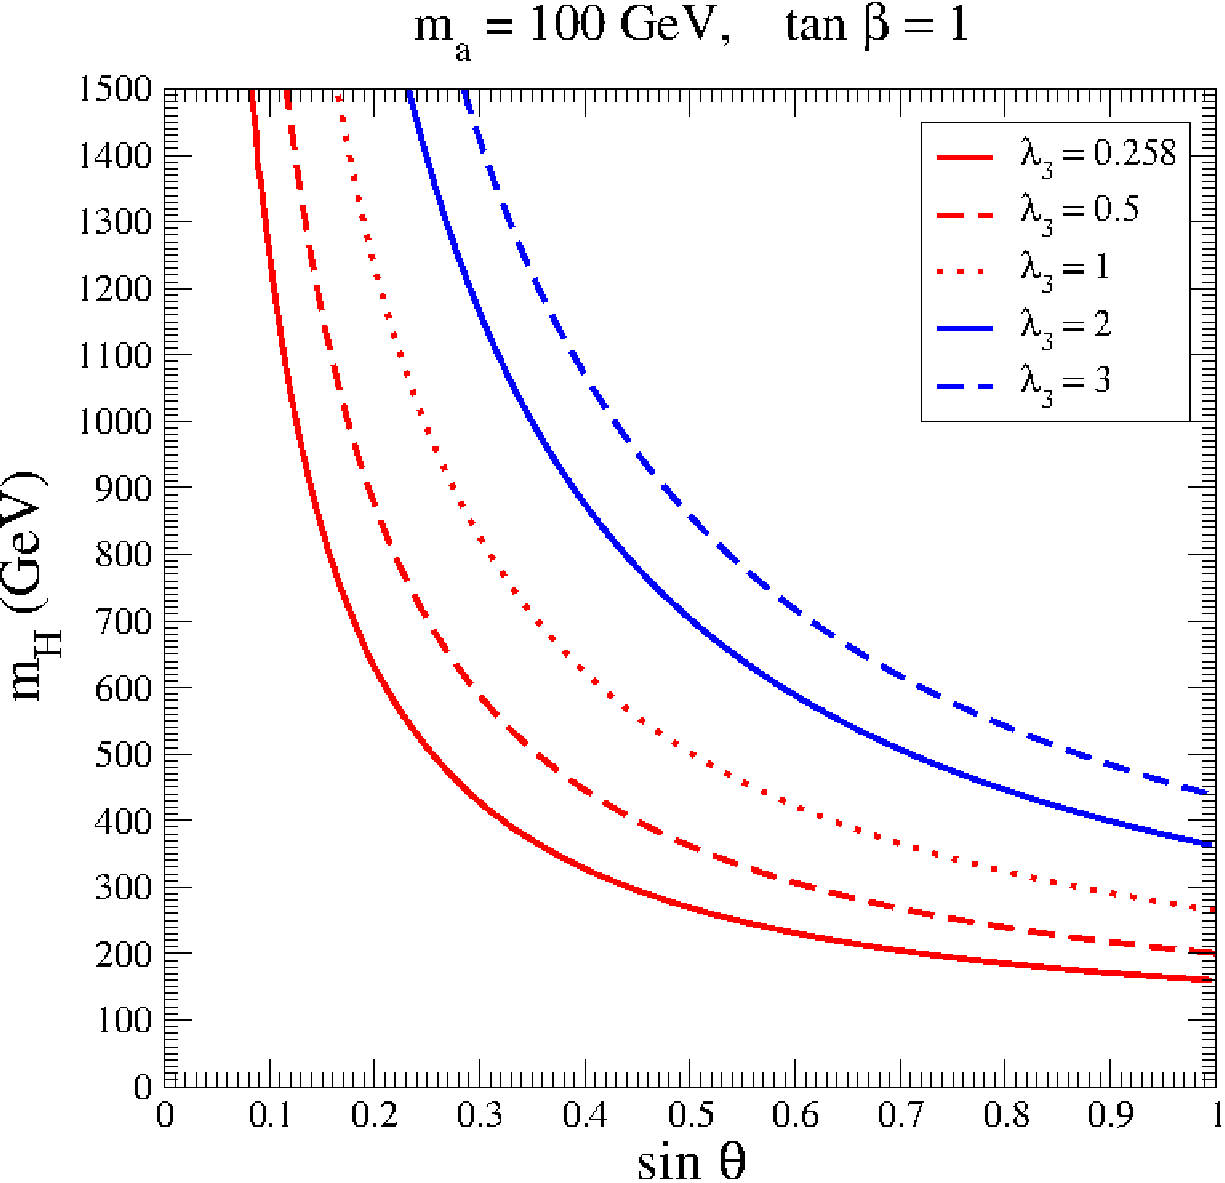
\includegraphics[width=0.485\textwidth]{texinputs/03_theoparameters/Figs/Plot_Eq.pdf}
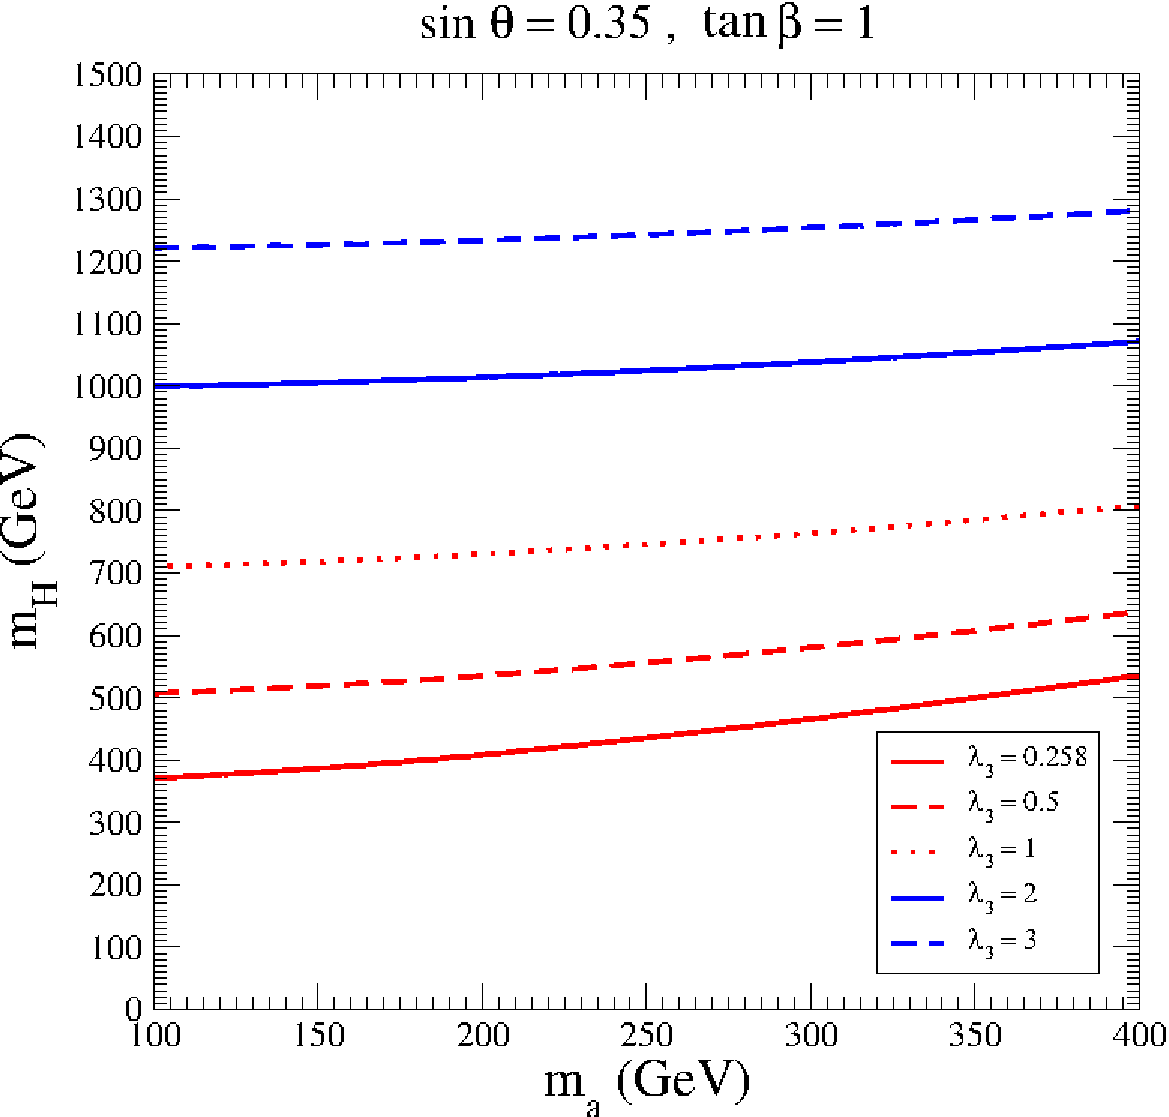
\includegraphics[width=0.485\textwidth]{texinputs/03_theoparameters/Figs/Plot_ma.pdf}
\caption{\small Regions of parameter space in the 
    ($m_a,\, m_{H_0}$) (left) and ($s_{\theta},\, m_a$) (right) planes for which the tree-level boundedness from below conditions~\ref{stability2HDM}
    are satisfied, assuming $m_{H^{\pm}} = m_{H_0} = m_{A_0}$. 
}
\label{Fig_Stability}
\end{center}

\vspace{-2mm}

\end{figure}
    %
    %
    
    Figure~\ref{Fig_Stability} shows that the region satisfying the tree-level boundedness from below conditions increases as $\lambda_3$ increases. At the same time, 
    the choice $\lambda_3 = \lambda_{P1} = \lambda_{P2}$ which we adopt in the present analysis allows the increase in $\lambda_3$  not to affect the mono-Higgs sensitivity
    via a change in the coupling $g_{aAh}$
    %
    \begin{eqnarray}
     g_{aAh} &=& \frac{c_{\theta} \,s_{\theta}}{m_{H} \,v} \left[m_h^2 + m_H^2 -m_a^2 - 2 
     (\lambda_3 - \lambda_{P1} c_{\beta}^2 - \lambda_{P2} s_{\beta}^2) v^2 \right] \nonumber \\
      &=& \frac{c_{\theta} \,s_{\theta}}{m_{H} \,v} \left[m_h^2 + m_H^2 -m_a^2 \right] 
    \end{eqnarray}
    %
    We then fix the value $\lambda_3 = 3$ as benchmark for the rest of our analysis. 
    
    \vspace{3mm}
    
    A few comments are in order. 
    
    \begin{itemize}
     \item The choice of $\lambda_3$, motivated by boundedness from below conditions, while not affecting the mono-Higgs sensitivity 
    if $\lambda_3 = \lambda_{P1} = \lambda_{P2}$, has an impact on the mono-$Z$ sensitivity since the coupling 
    %
    \begin{eqnarray}
     g_{Haa} &=& \frac{1}{m_{H} \,v} \left[ 2\, t_{2\beta}^{-1}\, s_{\theta}^2\, 
(m_h^2 - \lambda_3 v^2) + s_{2\beta}\, c_{\theta}^2 v^2 (\lambda_{P1} - \lambda_{P2}) \right] \nonumber \\
      &=& \frac{1}{m_{H} \,v} \left[ 2\, t_{2\beta}^{-1}\, s_{\theta}^2\, 
(m_h^2 - \lambda_3 v^2) \right] 
    \end{eqnarray}
    %
    does depend on $\lambda_3$ and influences the balance between $\Gamma(H_0 \to aa)$ and $\Gamma(H_0 \to Za)$ which ultimately determines the 
    $H_0 \to Za$ branching fraction. In short, the choice of $\lambda_3$, $\lambda_{P1}$, $\lambda_{P2}$ affects either mono-Higgs or mono-$Z$ sensitivities
    (or both).
    
    \item Together with boundedness from below, other potential constraints are usually considered in the context of the 2HDM and apply in general, 
    among them unitarity (see e.g.~\cite{Ginzburg:2005dt,Grinstein:2015rtl}) and absolute stability of the electroweak vacuum (see e.g.~\cite{Barroso:2013awa}). 
    In the present context we find these constraints 
    are generically weaker than the boundedness from below condition and therefore disregard them in the following. 
    
    \item The boundedness from below conditions are here evaluated at tree-level, but in a fully consistent treatment 
    they should be evaluated including the effect of radiative corrections. This is however 
    a much more involved process than what has been discussed above for the 
    tree-level case (see e.g.~\cite{Staub:2017ktc}). In addition, 
    the boundedness from below constraints discussed here are potentially sensitive to the 
    existence of UV physics which our 2HDM+S simplified does not capture, and which could modify the above picture through the presence of higher-dimensional 
    operators. Still, it is worth pointing out that for the 2HDM+S simplified model to be a good description of LHC phenomenology we require 
    the new physics scale suppressing these effective operators to be above the TeV scale (since in our scans we are considering scalar masses up to $\sim 1$ TeV), 
    and thus the presence of these high-energy operators is not expected to be of much help in case a runaway field direction exist at tree level in the 2HDM scalar 
    potential.
    \end{itemize}
    
    
    
    
\end{itemize}

\section{Model kinematics}
The signature and kinematic distributions of the \hdma model at colliders are determined by the values assigned to the parameters described in the previous chapter. 
The model parameters can affect the total signal cross-section, the kinematic distributions, or both. 
In order to obtain a representative grid of benchmark points for collider searches and reduce this multi-dimensional parameter space, we scan ranges of the possible values of these parameters and observe the impact on the kinematic distributions for representative collider searches.

%Since the generation and simulation of model points is time-consuming and computationally expensive, it is important to choose a that gives a unique set of kinematic distributions. 

In this chapter, we will first outline the main experimental searches that can be used to search for the 2HDM+P model, and present the distributions of the kinematic variables for each of the searches as a function of the free parameters of the 2HDM+P model. We note that in the following we have chosen to fix the DM coupling  $y_\chi$ to unity, and $\lambda_{P1} = \lambda_{P2} = \lambda_P = 3$ as explained in \autoref{sub:vacuumStability}.  
%TODO: explain why unity?

%description of searches
\subsection{Experimental searches}

\paragraph{Signatures including a Higgs boson }

\subparagraph{\monohbb signature}. The results in this and in the following section are at parton level. 
 
\cite{Aaboud:2017yqz}

\paragraph{Signatures including a Z boson}

Events with a Z boson and \MET may signal the presence of invisible particles recoiling against the Z boson~\cite{Carpenter:2012rg,Bell:2012rg}. 
LHC analyses (e.g.~\cite{Aaboud:2017bja,Sirunyan:2017qfc} for the most recent ones), the DM interpretations of the analysis results have focused on either invisible decays of the SM-like Higgs bosons or topologies where the Z boson is produced as initial-state radiation (ISR) from a quark. The ISR-based topologies generically favor radiation of a gluon or photon rather than a massive gauge boson, thus limiting the discovery sensitivity of a Z-based approach compared to monojet and mono-photon searches. In contrast, the model studied in this document generates the mono-Z signature dominantly via the all-bosonic H-a-Z vertex, which can lead to enhancements in the mono-Z sensitivity compared to jet and photon signatures. 

\subparagraph{Mono-Z (leptonic) signature}

%TODO: add a short paragraph on the relative importance of leptonic and hadronic channels
Three consecutive stages of event selection are considered in the case the Z decays leptonically:

\begin{itemize}
\item Inclusive: Lepton \pt and $\eta$ requirements corresponding to the typical experimental trigger acceptance are applied.
\item Preselection: A dilepton candidate with an invariant mass in a window around the Z mass is required, and a minimum transverse momentum of the $\chi\overline{\chi}$ system is required.
\item Final selection: Requirements on the main discriminating variables used in the relevant analyses are added: The angular separation in the transverse plane between the $\chi\overline{\chi}$ and \lp\lm systems $\Delta\Phi(ll,\MET)$, the relative transverse momentum difference between them $|p_{T,ll} - \MET|/p_{T,ll}$ and the angular separation between the leptons $\Delta R(ll)$. Additionally, the \MET requirement is tightened.
\end{itemize}

The exact event selection criteria are listed in the appendix, in \autoref{tab:monozll_selection}. The results in this and in the following section are at particle level. 

\subparagraph{Mono-Z (hadronic) signature}

The hadronic signature in $Z$+\MET events ($Z \to q\bar{q}$ decays in association with large missing transverse momentum) is complementary to the leptonic signature. 
Hadronic decays are more frequent than leptonic decays, but suffer from larger backgrounds. For these reasons, the $Z$ (hadronic) + \MET search is favored if the model include higher mass scalar and pseudoscalar bosons. 
%TODO: this is pretty sloppy...

The event selection in this case changes depending on the production transverse momentum of the Z-boson, as in the case of the exchange of a high-mass CP-even $H$ boson. 
If the Z-boson is boosted, then its hadronic decay products could be merged into a single jet, and the $Z$ to QCD background discrimination can be improved by exploiting the presence of substructure within a single, large-radius jet (denoted by $J$). 
The \textit{boosted} search is performed in addition to the \textit{resolved} search, where the $Z$ decay products are reconstructed as two separate small-radius jets (denoted by $j$).

\paragraph{Event selection :} 
For mono-$Z (\to q\bar{q})$ events intermediated by the exchange of a high-mass CP-even $H$ boson, 
the $Z$-boson will be produced with 
a large transverse momentum and the hadronic decay products of such $Z$-boson could be merged into a single jet. 
Such ``boosted'' event topology is investigated by exploiting the reconstruction technique with 
a large-radius jet (denoted by $J$), 
in addition to more conventional ``resolved'' event topology where the $Z$ decay products are reconstructed 
as two separate
small-radius jets (denoted by $j$). The jet reconstruction and the following analysis are all performed at particle level
after showering and hadronization implemented in Pythia 8.212 described above.

Two consecutive stages of event selection are considered for the boosted and resolved event topologies:
\begin{itemize}
\item Inclusive: minimal kinematic requirements are applied to a pair of small-radius jets (a single large-radius jet) 
for the resolved (boosted) event topology. 
These selection criteria are applied separately, i.e, not sequentially.
\item Final selection: selection criteria are applied to the a number of variables. 
The invariant mass of the pair of small-radius jets or the single large-radius jet is required to be within a window around the $Z$ mass. 
In addition, selection is applied to the azimuthal angular difference between the $\chi\overline{\chi}$ and the hadronic $Z$-boson system, $\Delta\Phi(jj {\,\text{or}\,} J, \MET)$, and the magnitude of $\MET$.
These final selection cuts are applied sequentially to mimic a realistic analysis; in this study the boosted selection cuts are applied first and then the resolved selection cuts are applied to those events that fail the boosted ones.
\end{itemize}

The exact event selection criteria are listed in the appendix, in \autoref{tab:monozqq_selection}. The results in this and in the following section are at particle level. 

\paragraph{Signatures including heavy flavor quarks}

Heavy flavor final state can have sizable contributions to the production of the CP-even and CP-odd scalar mass eigenstates, due to the Yukawa structure of the couplings in the SM sector. 

%Add example cuts of the analysis

\subsection{Kinematic distributions}

%representative distributions varying each of the parameters
%Martin: ($m_\chi\,,\,\,M_a\,,\,\, t_\beta\,, \,\, M_H\,\,\text{or}\,\,M_A\,\,, \,\, y_\chi\$).
%Linda: We will count the low energy model parameters as consistent with  reference \cite{Bauer:2017ota}. The model parameters will consist of six particle masses $m_{H^{\pm}}$, $m_{H^{0}}$, $m_{A}$, $m_{a}$, $m_{h}$; three mixing angles $\alpha$, $\beta$, $\theta$; and three quartic couplings $\lambda_3$, $\lambda_{H1S}$,$\lambda_{H2S}$.

\subsubsection{Masses of the $H$, $A$ and $a$  bosons ($\mH$, $\mA$ and $\ma$)}

The masses $\mA$ and $\ma$ of the pseudoscalars $A$ and $a$, which represent the two mediators in \autoref{fig:feyn_hdm}, affect the shape of the $\MET$ distribution.  

In the mono-Z and mono-H channels, the main production contribution is from the $2\to1\to2$ processes $gg\to A\to a h$, and $gg\to H\to a Z$, respectively, with the light pseudoscalar decaying invisibly as $a\to \chi\chi$. In this case, the $A/H \to a h $ process produces a resonance in the invariant mass distribution of the final state system with a width determined by the widths of $a$, $A/H$, and of the SM bosons. This results in a peak in the transverse momentum distribution of the DM system, reconstructed as $\MET$ in the detector.

The location of this Jacobian peak can be calculated analytically starting from the masses of the particles involved in the decay~\cite{Bauer:2017ota}:

\newcommand{\mAH}{\ensuremath{M_{A/H}}\xspace}
\begin{align}
E^{\mathrm{miss},max}_T \approx \frac{\sqrt{\left(\mAH^2 -\ma^2 -M_{h/Z}^2\right)^2 - 4 \ma^2 M_{h/Z}^2}}{2\mAH}\,.
\label{eq:monoH_peak_met}
\end{align}

Thus, increasing $\mAH$ results in  a Jacobian peak at higher $\MET$, as shown in \autoref{fig:monoHbb_mA_scan_met}, \autoref{fig:monoz_ll_mA_scan} and \autoref{fig:monozhad_kin_inc_fixed_ma}.
Conversely, models with higher $\ma$ have a Jacobian peak at lower $\MET$, as indicated in \autoref{fig:monoHbb_ma_scan_met} and \autoref{fig:monozhad_kin_inc_fixed_mA}. 
For $\mAH\approx\ma+m_{Z/h}$, both the $a$ and Z/h bosons are produced approximately at rest, leading to an event population with overall low boost. 
These qualitative trends are consistent with the distributions of the other main selection variables as shown in the appendix (\autoref{app:extraKinematics}).

%Models with higher $\ma$ have softer \met (cf. \autoref{eq:monoH_peak_met})
%Models with a larger $\mA-\ma$ splitting have harder \met (cf.\autoref{eq:monoH_peak_met}).

%Mono-Z text:
%After applying the preselection requirements, scans of the model parameters are performed.  For this paper a subset of models are studied where \mA is degenerate with \mH.  Similar to mono-h, for mono-Z in the region $\mA>\ma$ a resonantly produced heavy scalar, $H$, decaying to $aZ$ produces a characteristic Jacobian peak in the \MET distribution.  The location of the peak depends on \mH and \ma as given by equation \autoref{eq:monoZ_jacobian_peak}, and the peak's width generally increases with values of  $\ma$ and $\mA$.  

%Figure \autoref{fig:monoz_ll_mA_scan} shows the Jacobian peaks for increasing values of \mH and fixed \ma for the Z + \MET searches. The position of the Jacobian peak in the \MET distribution depends on the values of \mH, \ma, and $M_{Z}$. Increasing the difference between \mH and \ma shifts the location of the peak towards high energies, whereas for small mass splittings the \MET distribution is soft and most events will fail to pass the \MET selection criteria.
%Significant portions of the spectrum are situated at relatively high boosts ($\MET>\unit[200]{GeV}$), which is more easily accessible experimentally.  
%This behavior is contrasted by the distributions in the inverted mass regions, which have nearly no distinct features and are mainly located at low mediator \pt. 
%The position of the Jacobian peak in the \MET distribution depends on the values of \mH, \ma, and $M_{Z}$. Increasing the difference between \mH and \ma shifts the location of the peak towards high energies, whereas for small mass splittings the \MET distribution is soft and most events will fail to pass the \MET selection criteria. 


\begin{figure}%[!htbp]
	\centering

	\begin{subfigure}[t]{0.48\textwidth}
	\centering
	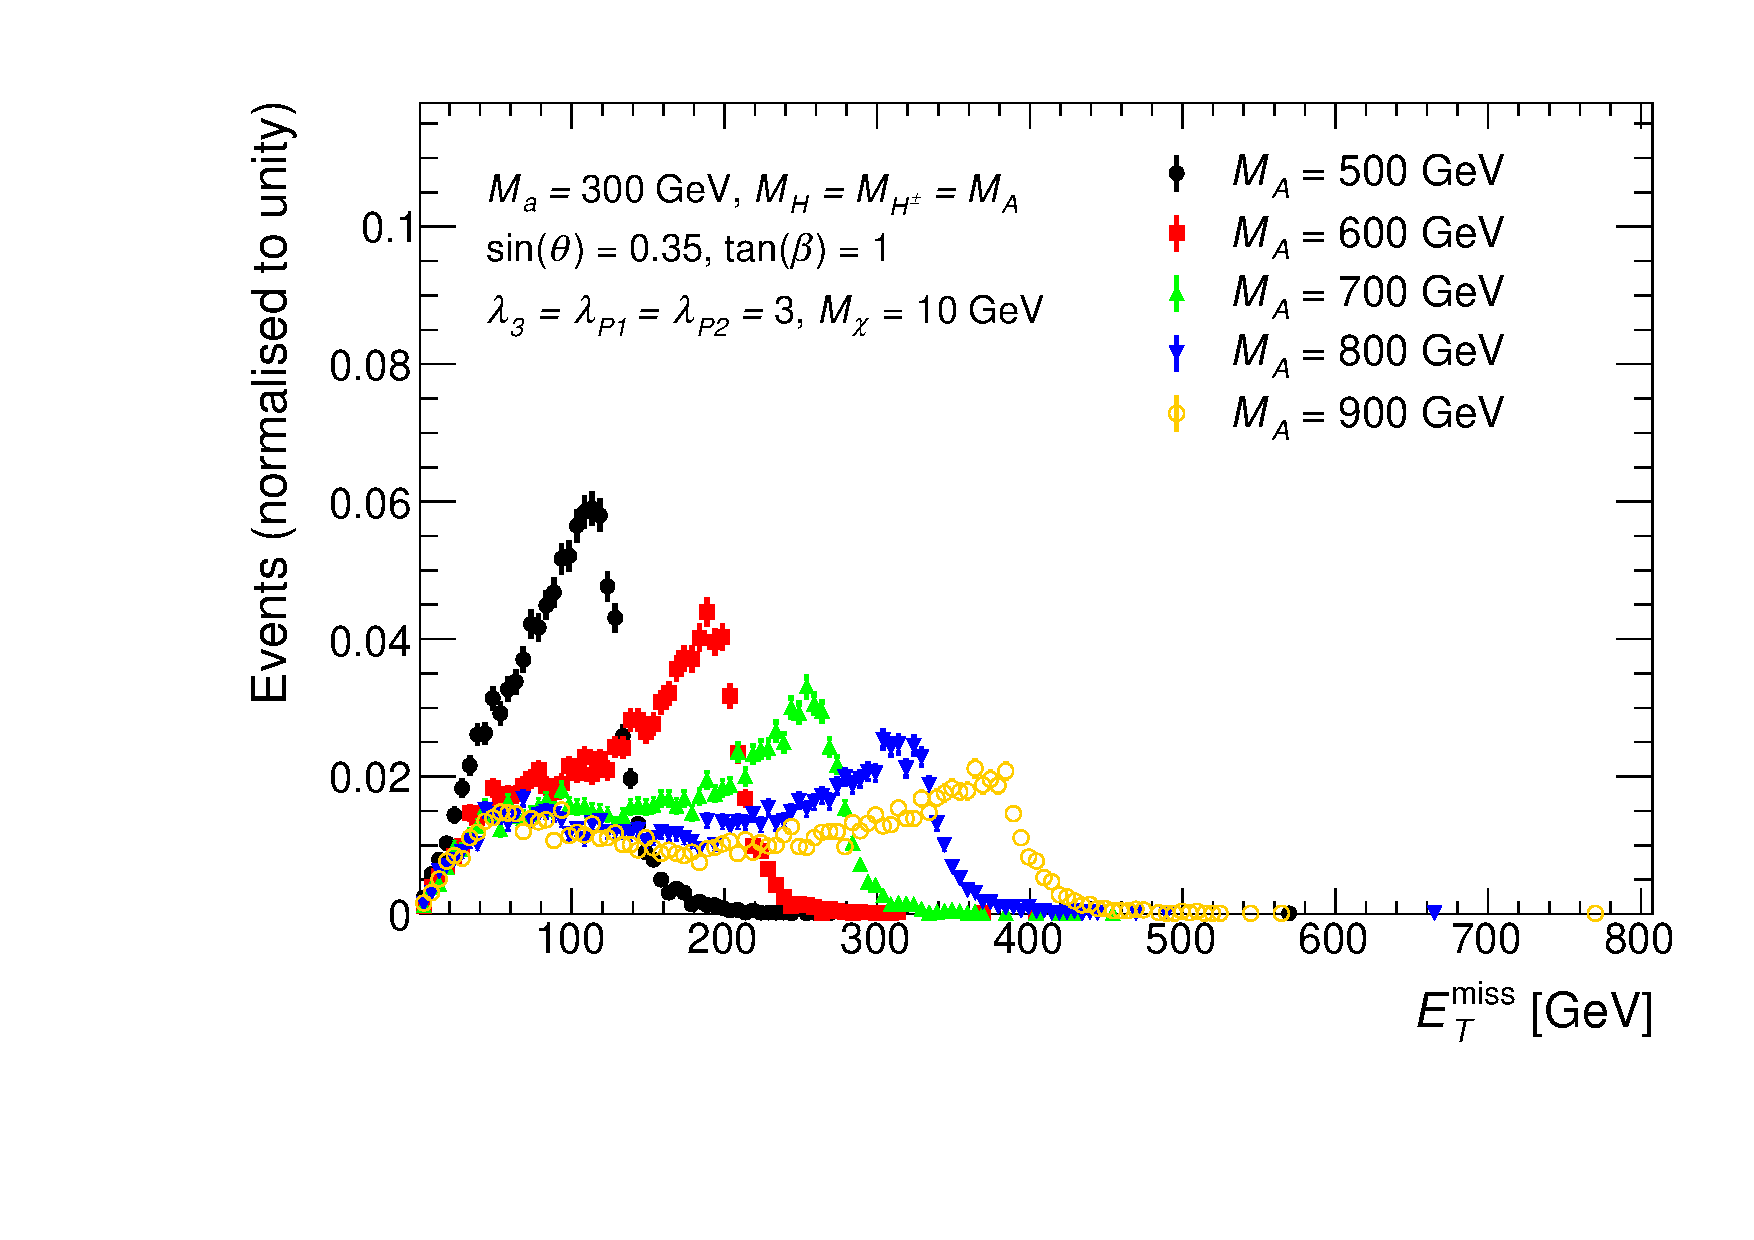
\includegraphics[width=\textwidth]{texinputs/04_grid/figures/monoHbb_m_large_A_scan_MET_liny_norm2one.pdf}
	\caption{$\MET$ distribution for points with different $\mA~(=\mH=\mHc)$
    and fixed $\ma = 300$ GeV. 
	\label{fig:monoHbb_mA_scan_met}} 
    \end{subfigure}
    \begin{subfigure}[t]{0.48\textwidth}
	\centering
	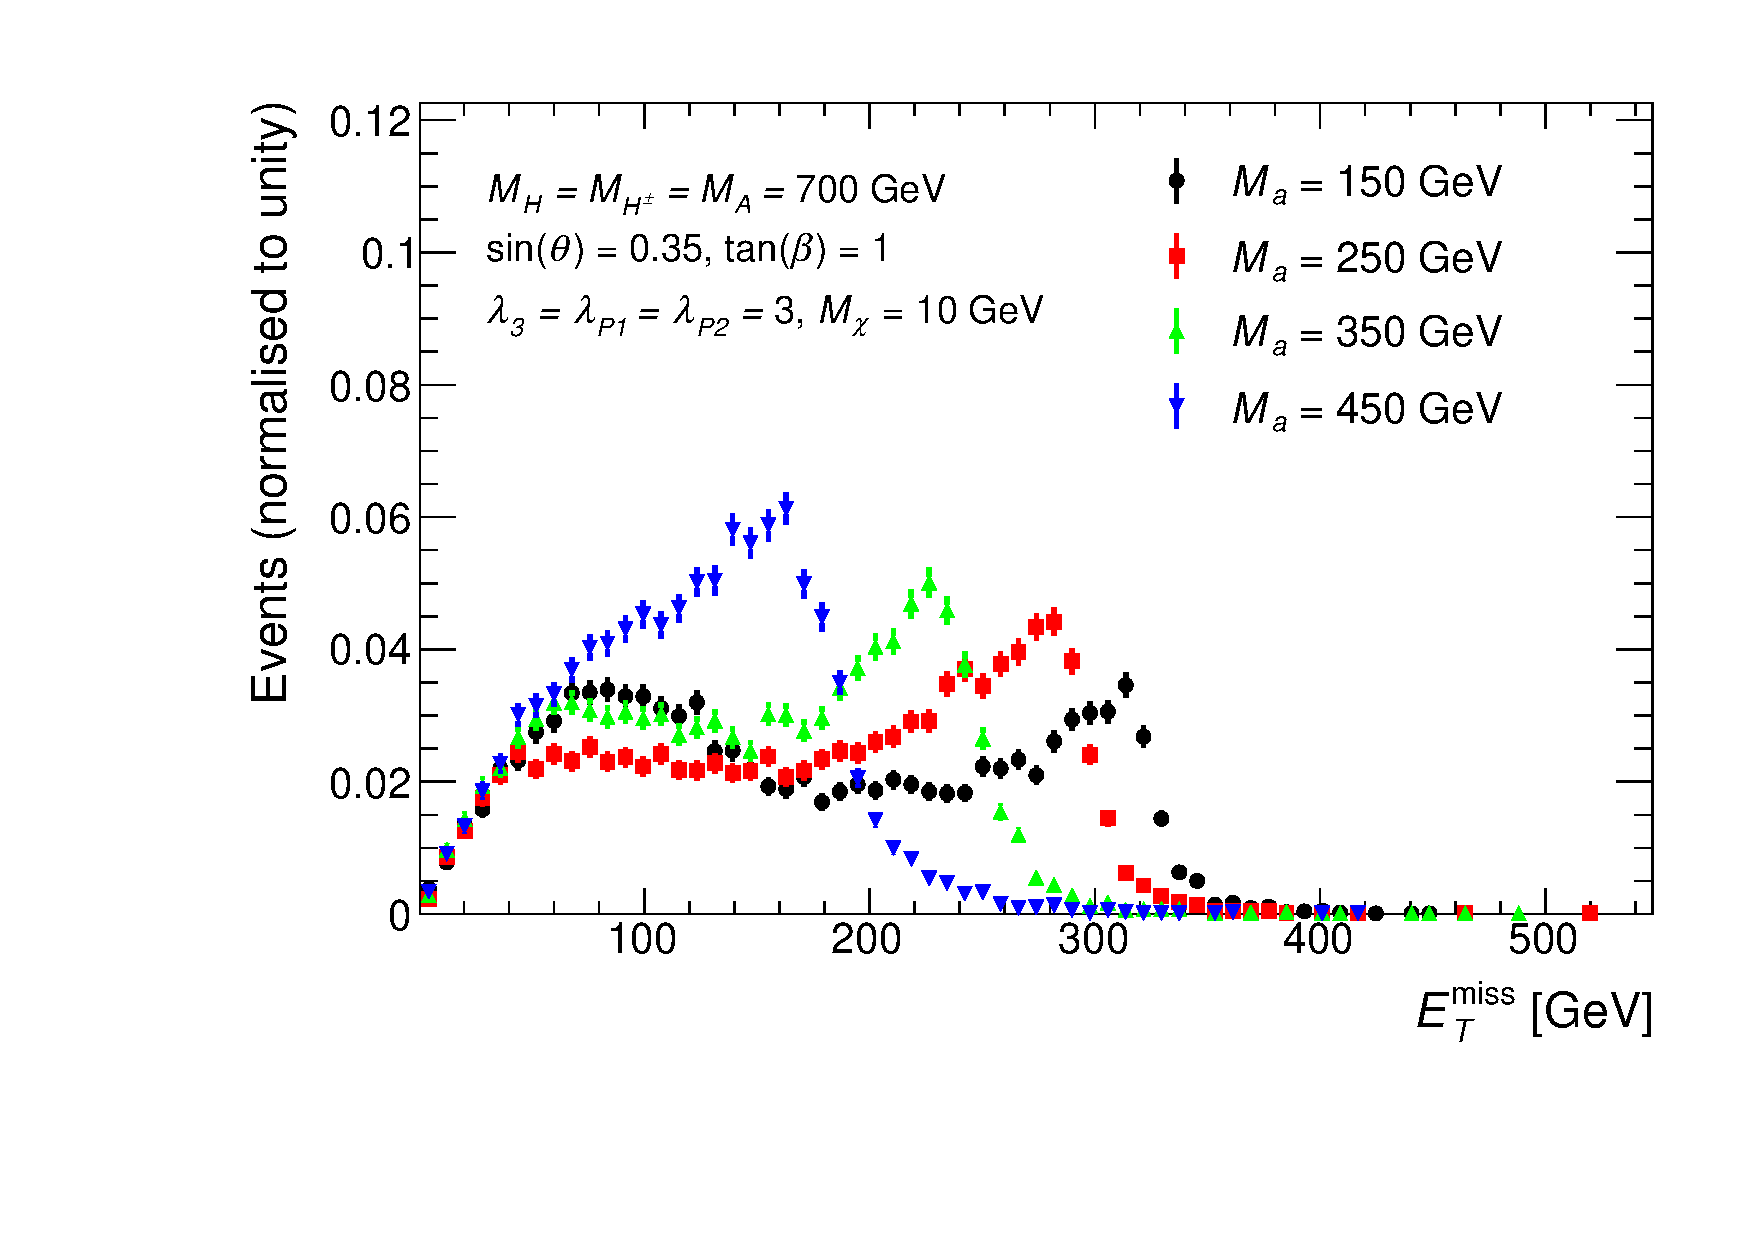
\includegraphics[width=\textwidth]{texinputs/04_grid/figures/monoHbb_m_small_a_scan_MET_liny_norm2one.pdf}	
	\caption{$\MET$ distribution for points with different $\ma$ and fixed $ \mA=\mH=\mHc= 700$ GeV. 
	\label{fig:monoHbb_ma_scan_met}}
    \end{subfigure}
    
    \caption{Parton-level $\MET$ distribution in \monohbb events for different $\ma$ and $\mA$, with $ \sinp = 0.35, \tanb = 1, \mDM = 10$ GeV and $ \lap1 = \lap2 = \lam3 = 3 $}
\end{figure}

\begin{figure}%[!htbp]
	\centering

    \begin{subfigure}[t]{0.75\textwidth}
	\centering
	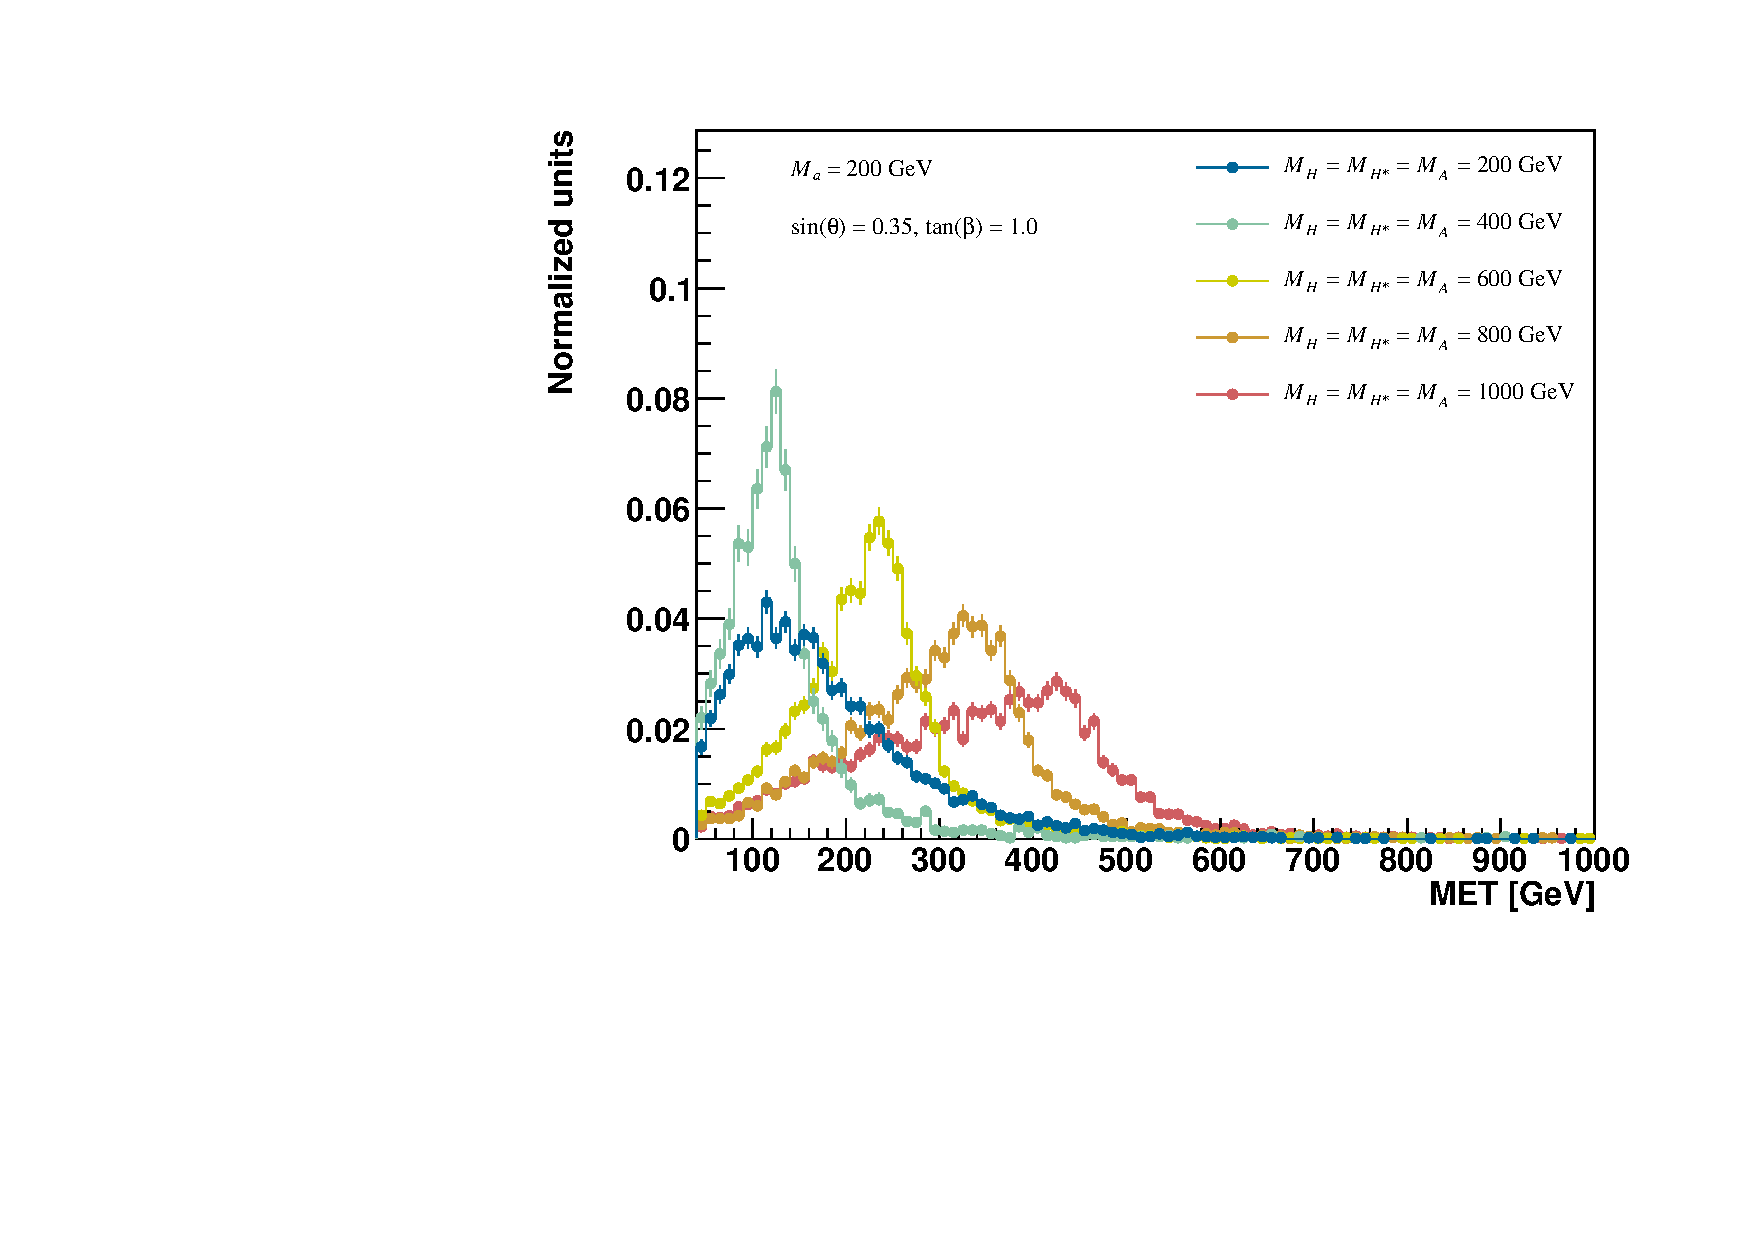
\includegraphics[width=\textwidth]{texinputs/04_grid/figures/monoz/leptonic/mAscan_for_ma200_axis.pdf}	
	\caption{The \MET distribution in signatures including a Z boson after preselection, with varying \mA values for fixed \ma = 200 GeV and \mA = \mH. \label{fig:monoz_ll_mA_scan}}
    \end{subfigure}

\end{figure}

\begin{figure}
\centering
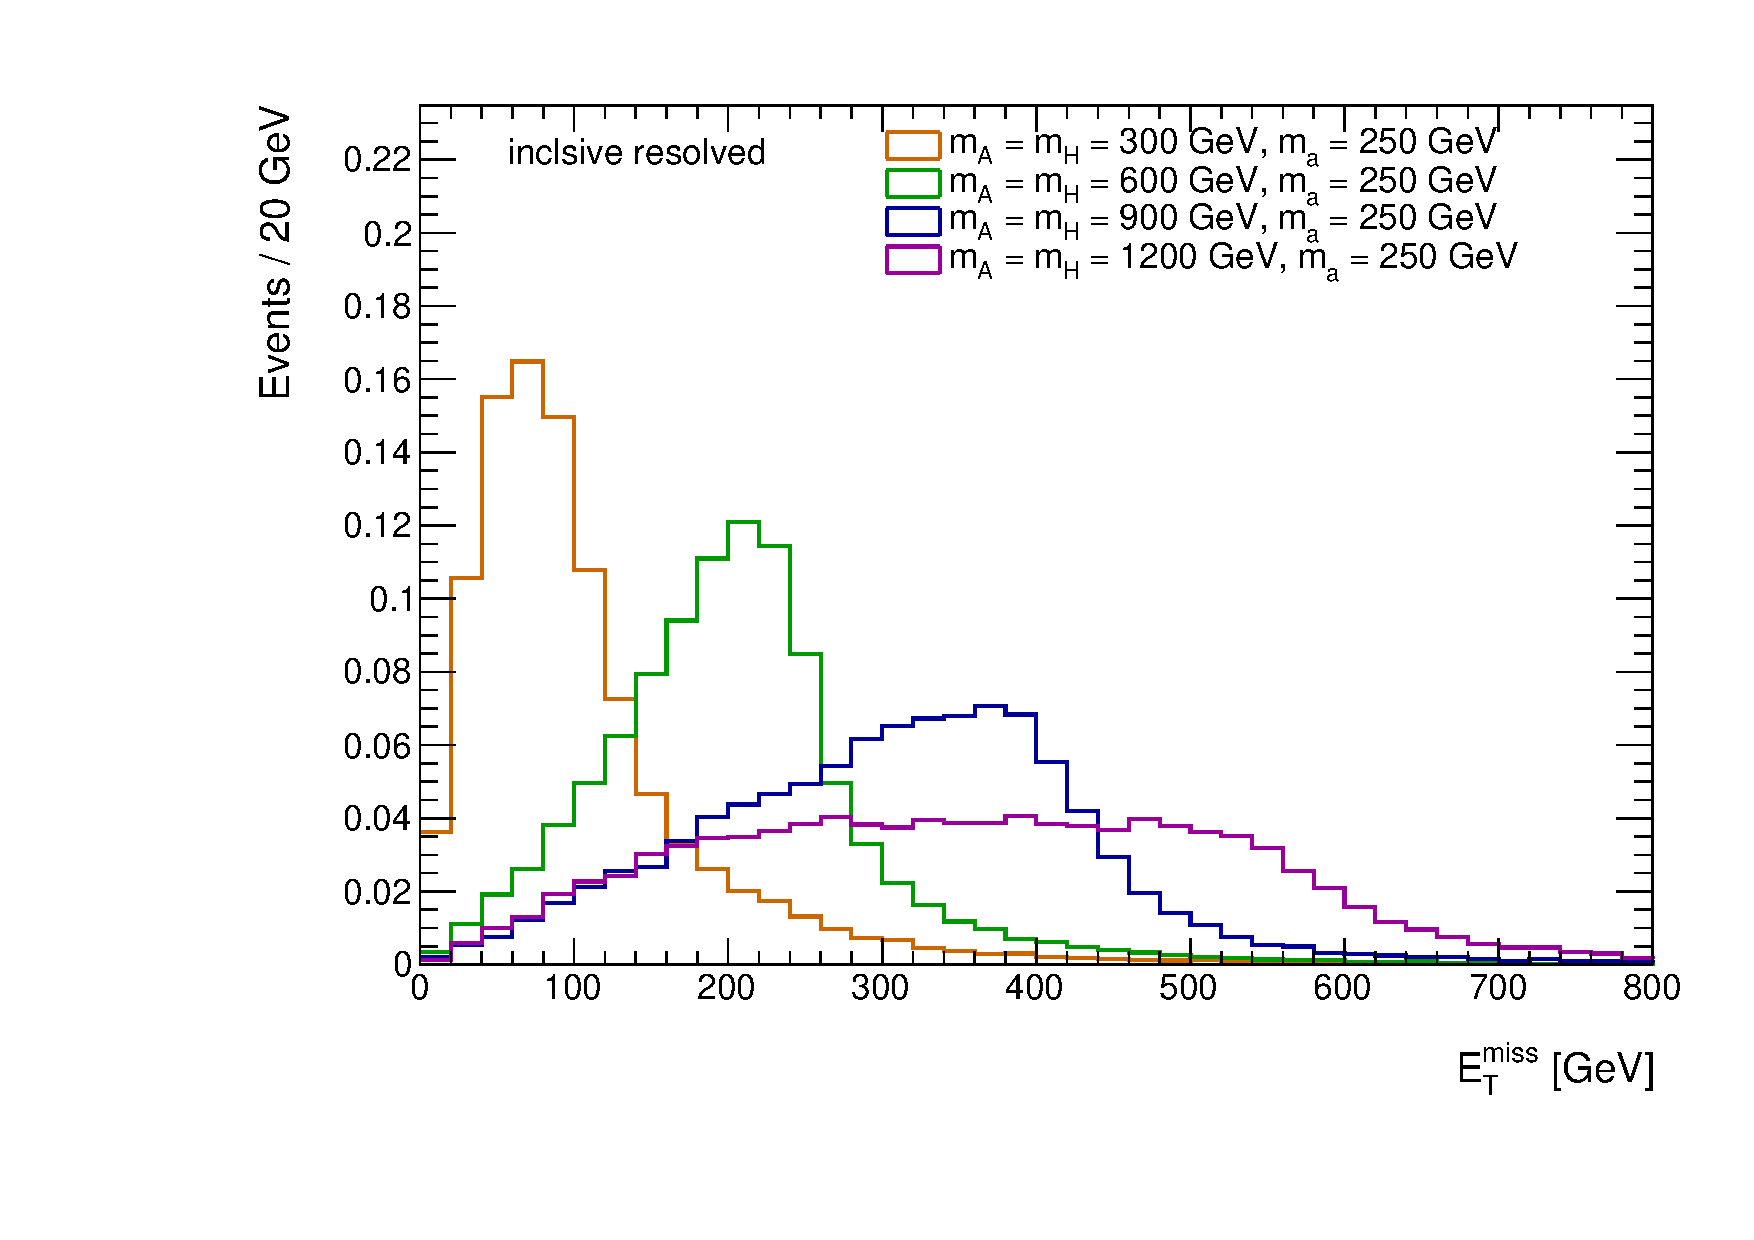
\includegraphics[width=0.45\textwidth]{texinputs/04_grid/figures/monoz/hadronic/ma250_incl_resl_MET_linear.pdf}
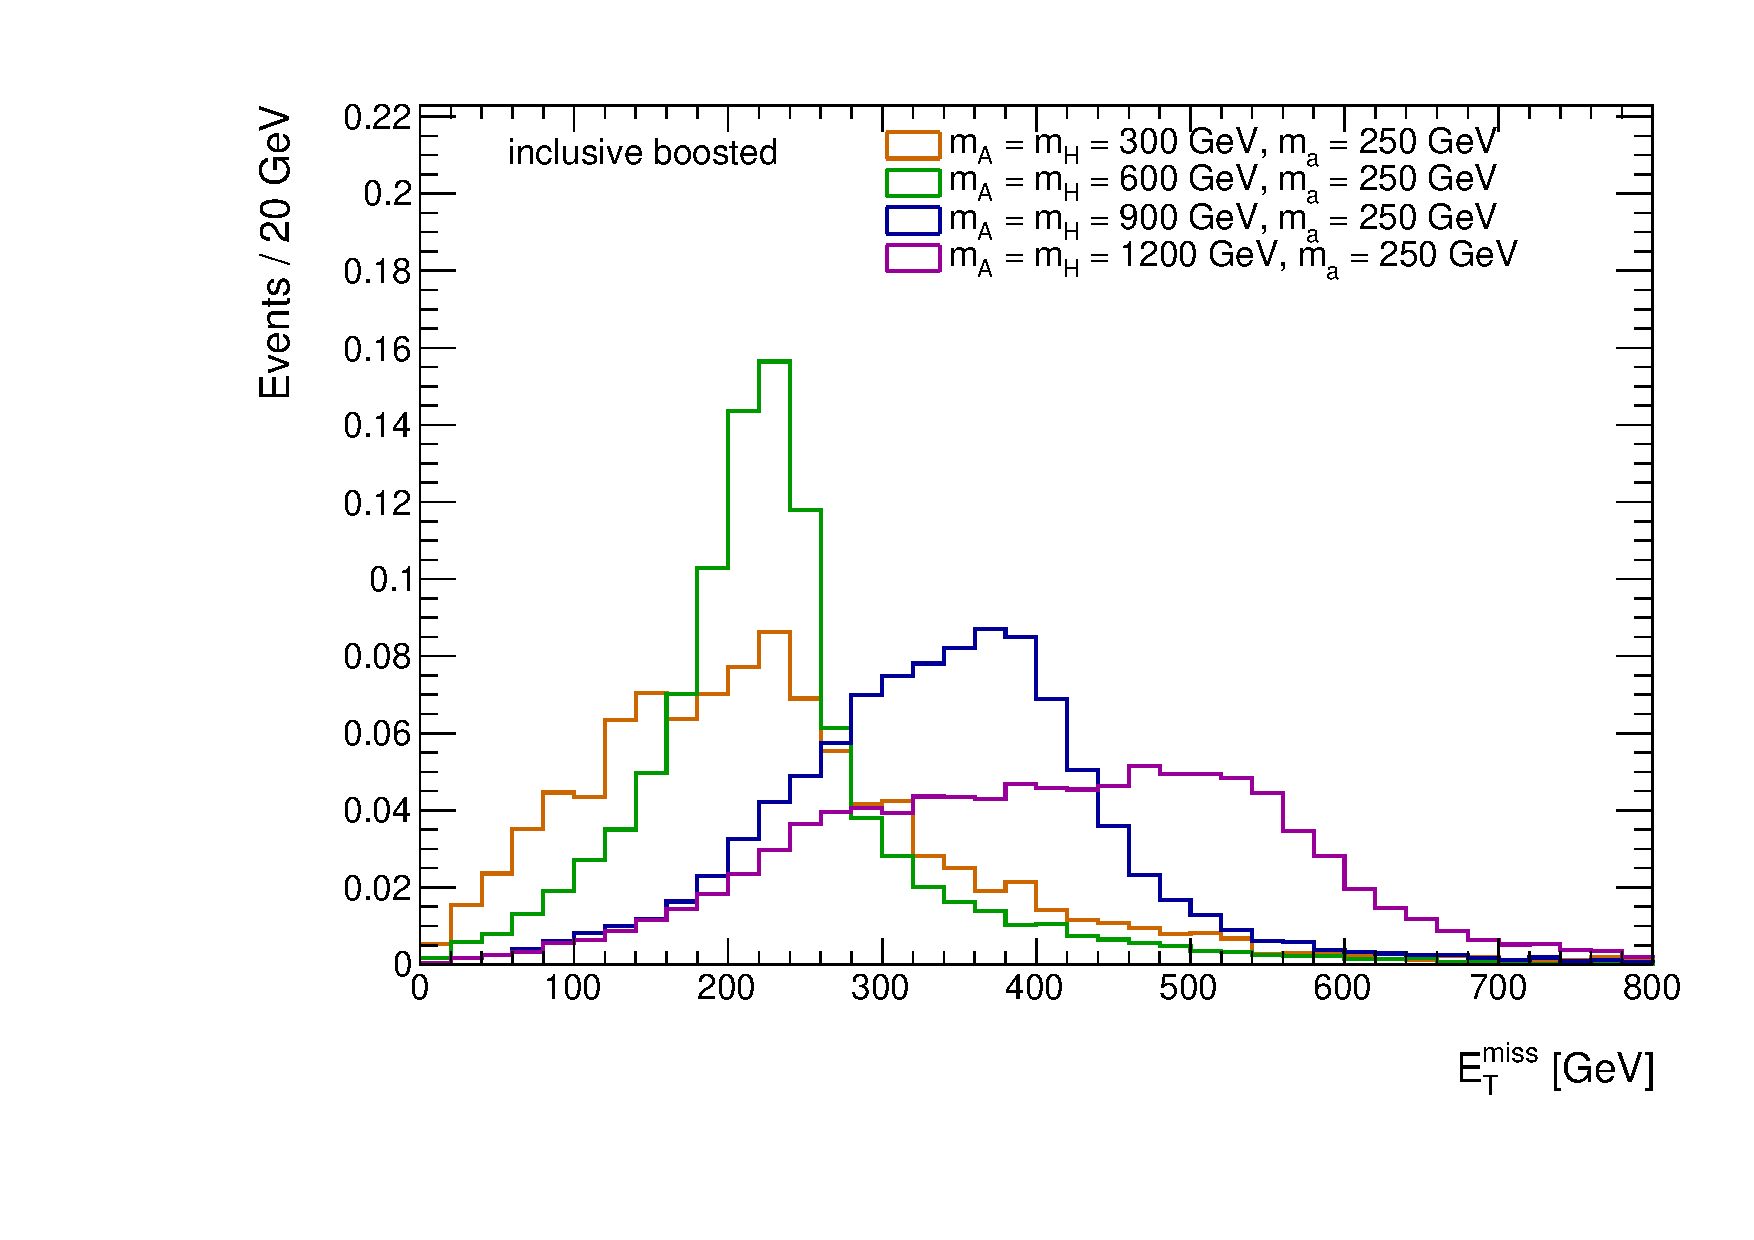
\includegraphics[width=0.45\textwidth]{texinputs/04_grid/figures/monoz/hadronic/ma250_incl_merged_MET_linear.pdf}
\caption{Dijet mass (top), $\Delta\Phi(jj, \MET)$ (middle) and $\MET$ (bottom) distributions 
after applying the inclusive selections in the resolved analysis are shown on the left side. Large-radius 
jet mass (top), $\Delta\Phi(J, \MET)$ (middle) and $\MET$ (bottom) distributions 
after applying the inclusive selections in the boosted analysis are shown on the right side. 
The signal masses are chosen to be \mA = 300, 600, 900 and 1200~GeV with the fixed \ma = 250~GeV.}
\label{fig:monozhad_kin_inc_fixed_ma}
\end{figure}

\begin{figure}
\centering
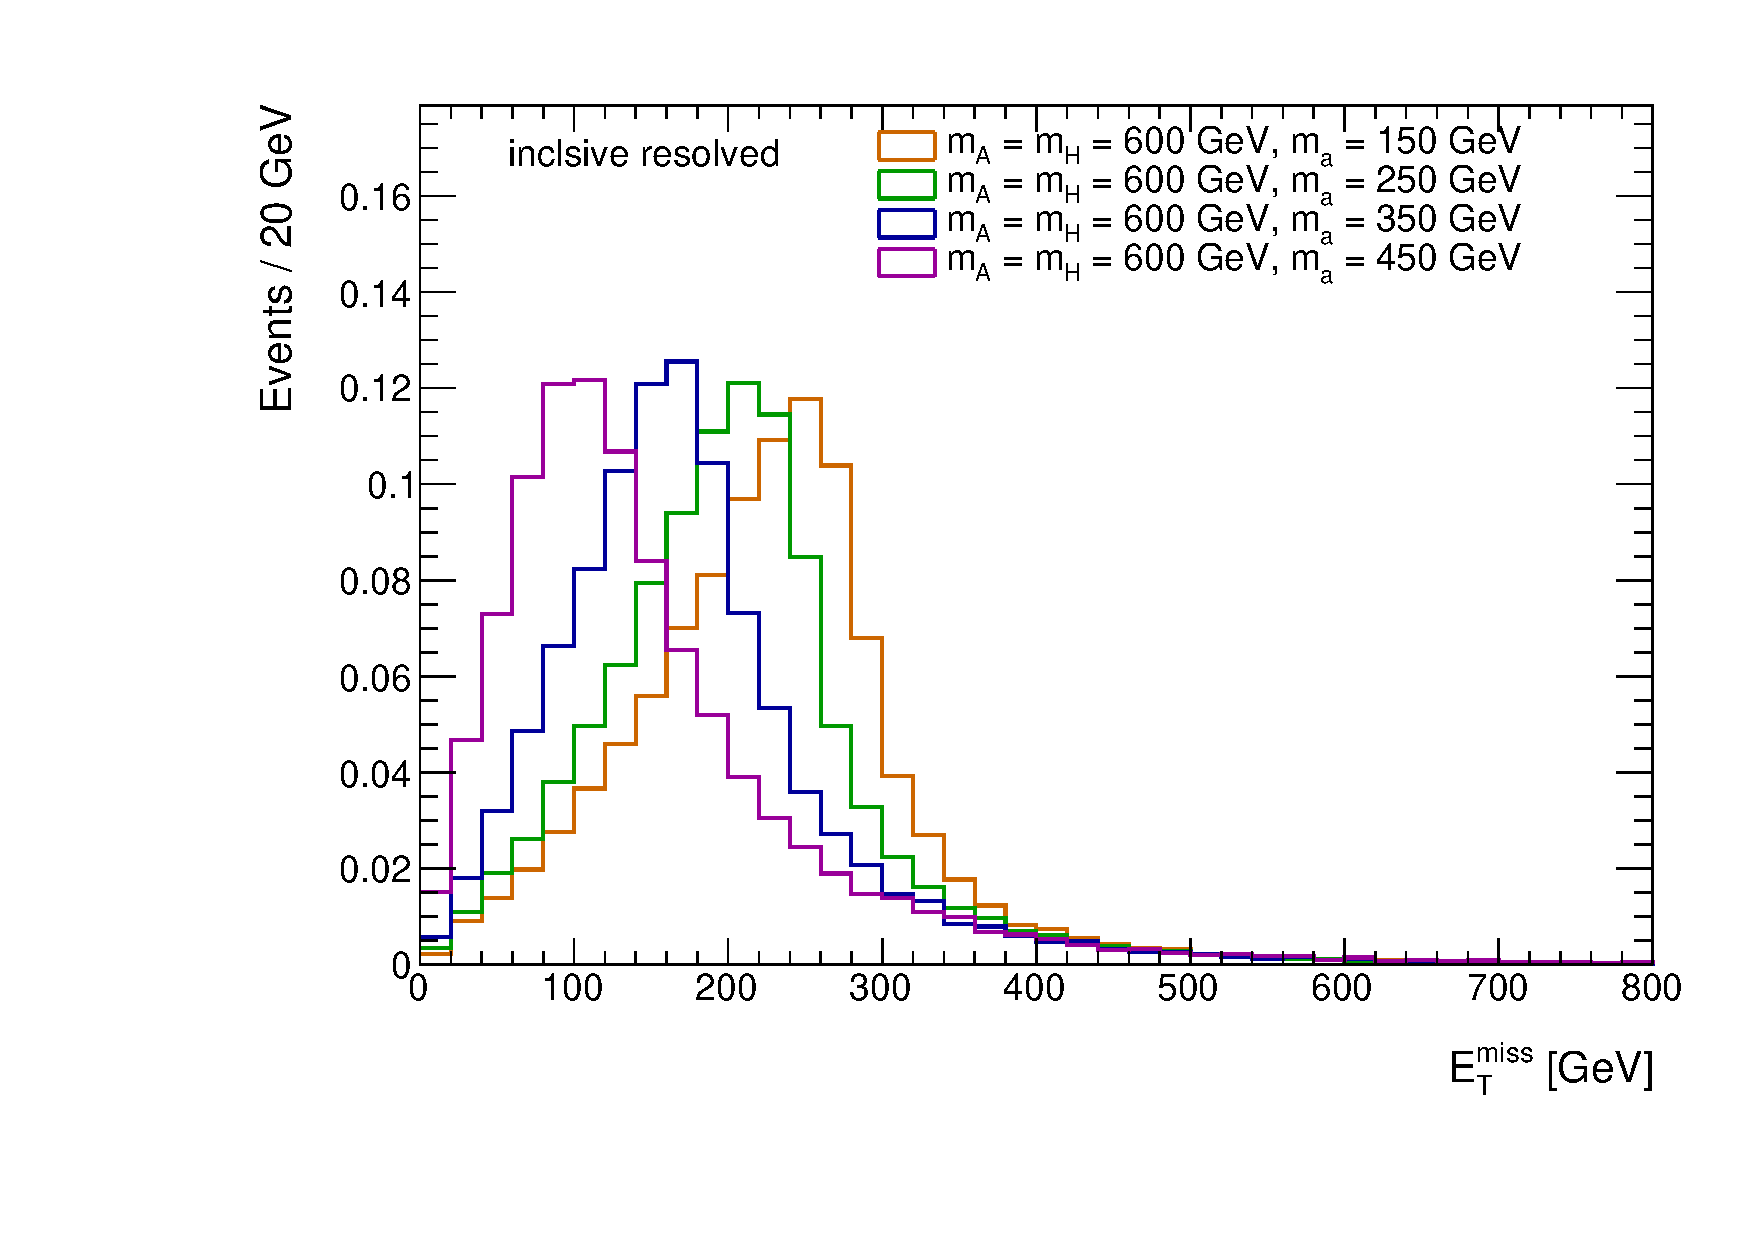
\includegraphics[width=0.45\textwidth]{texinputs/04_grid/figures/monoz/hadronic/mA600_incl_resl_MET_linear.pdf}
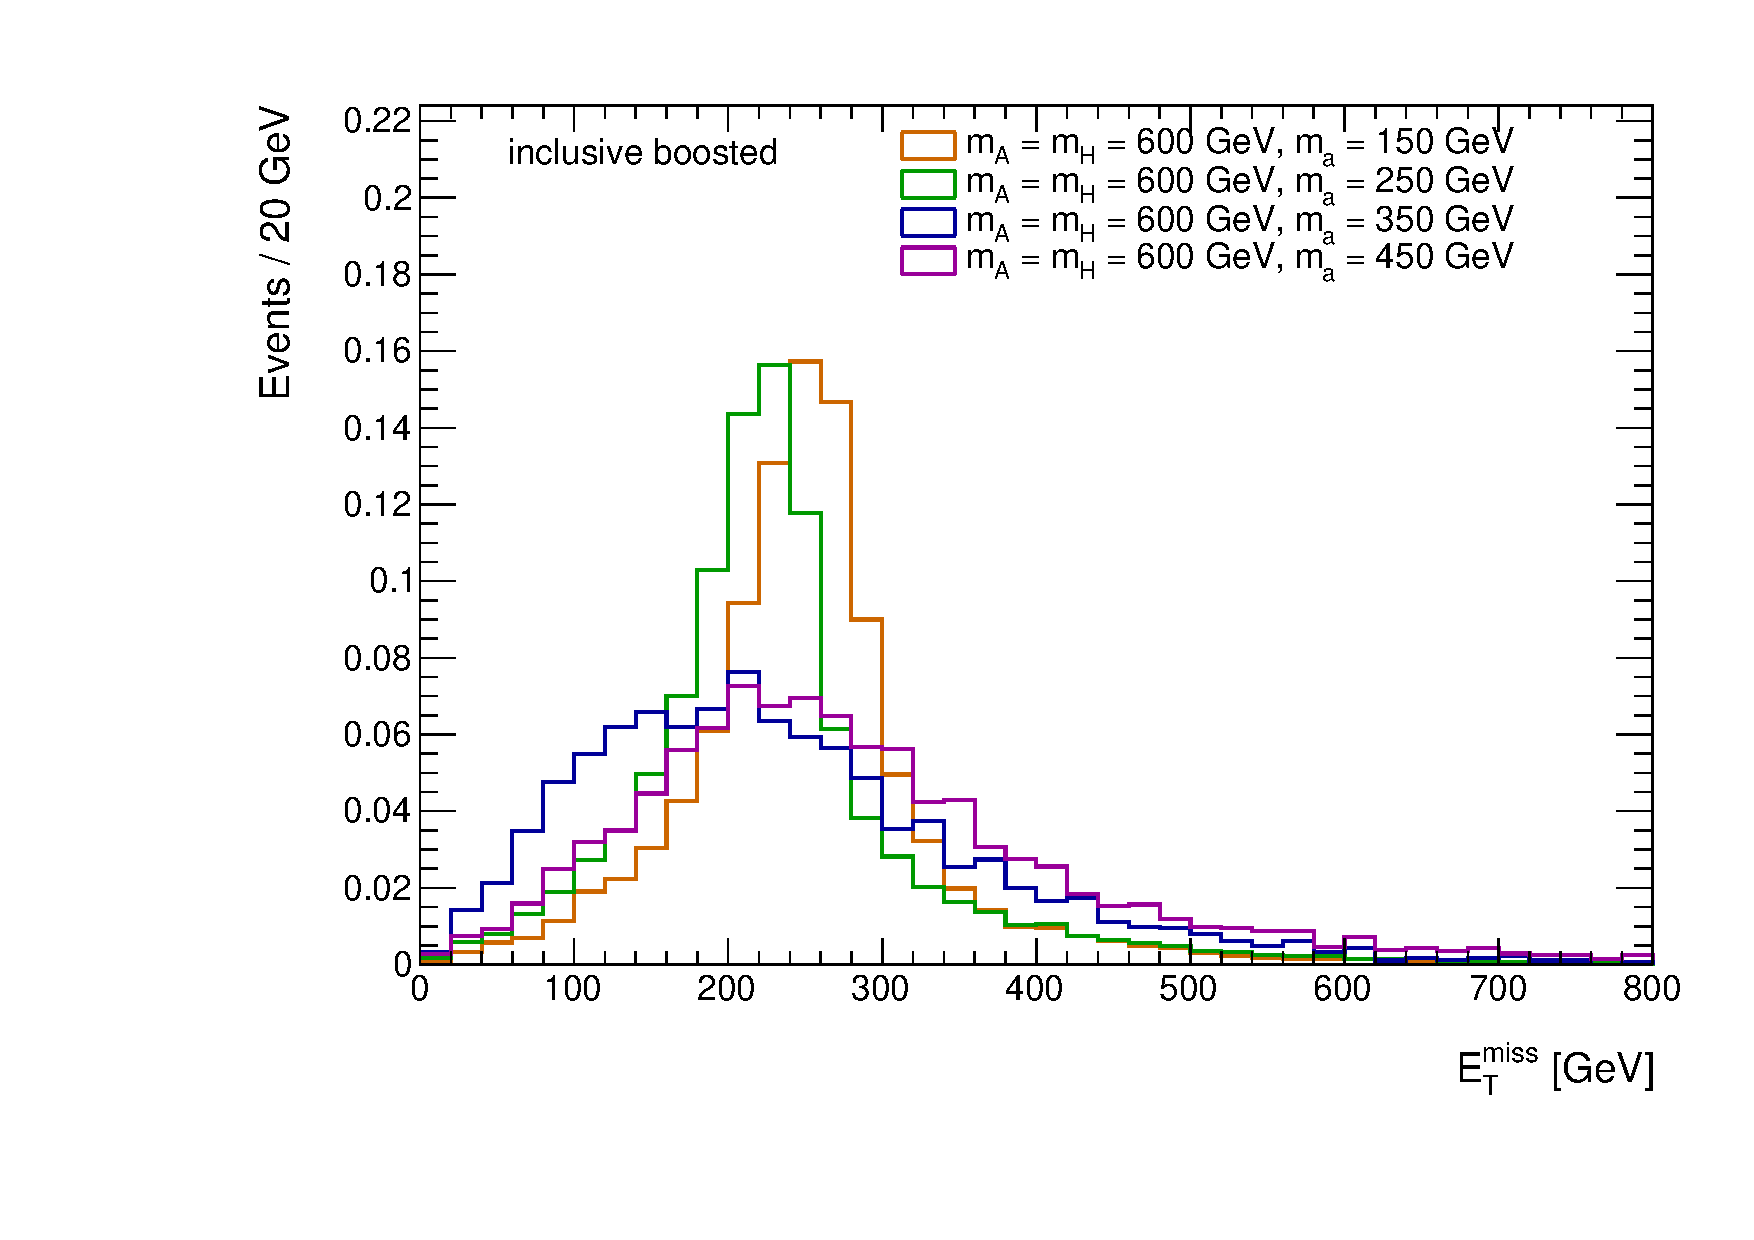
\includegraphics[width=0.45\textwidth]{texinputs/04_grid/figures/monoz/hadronic/mA600_incl_merged_MET_linear.pdf}
\caption{Z (hadronic) + \MET search $\MET$ distributions 
after applying the inclusive selections in the resolved analysis are shown on the left side, and on the right side
for the boosted analysis. The signal masses are chosen to be \ma = 150, 250, 350 and 450~GeV with the fixed \mA = 600~GeV.}
\label{fig:monozhad_kin_inc_fixed_mA}
\end{figure}

Some fraction of signal events is also produced in non-resonant $2 \to 3$ processes $gg \to h \chi \chi$, as in \autoref{fig:feyn_hdm_box}, leading to a broader distribution of the invariant mass of the decay products.  
%link into thereory section graph or cite paper
Consequently, this results in a broader and softer \met distribution that is distinct from the Jacobian peak discussed above, and contributes to the off-peak features of \autoref{fig:monoHbb_ma_scan_met} and \autoref{fig:monoHbb_mA_scan_met}. 

The masses \ma and \mA influence the kinematics in the $t\bar{t}$ + \MET signature as well. As shown in \autoref{fig:kin_Ma}, the $E_{T}^{miss}$, and leading and trailing top quark $p_{T}$ distributions broaden with increasing $\mathrm{M_{a}}$. Similarly, for values of $\mathrm{M_{A}} < \mathrm{M_{a}}$, as $\mathrm{M_{A}}$ increases, the kinematic distributions mentioned above also broaden, as shown in \autoref{fig:kin_MA}.

\begin{figure}
  \centering
  \begin{subfigure}[b]{0.49\textwidth}
    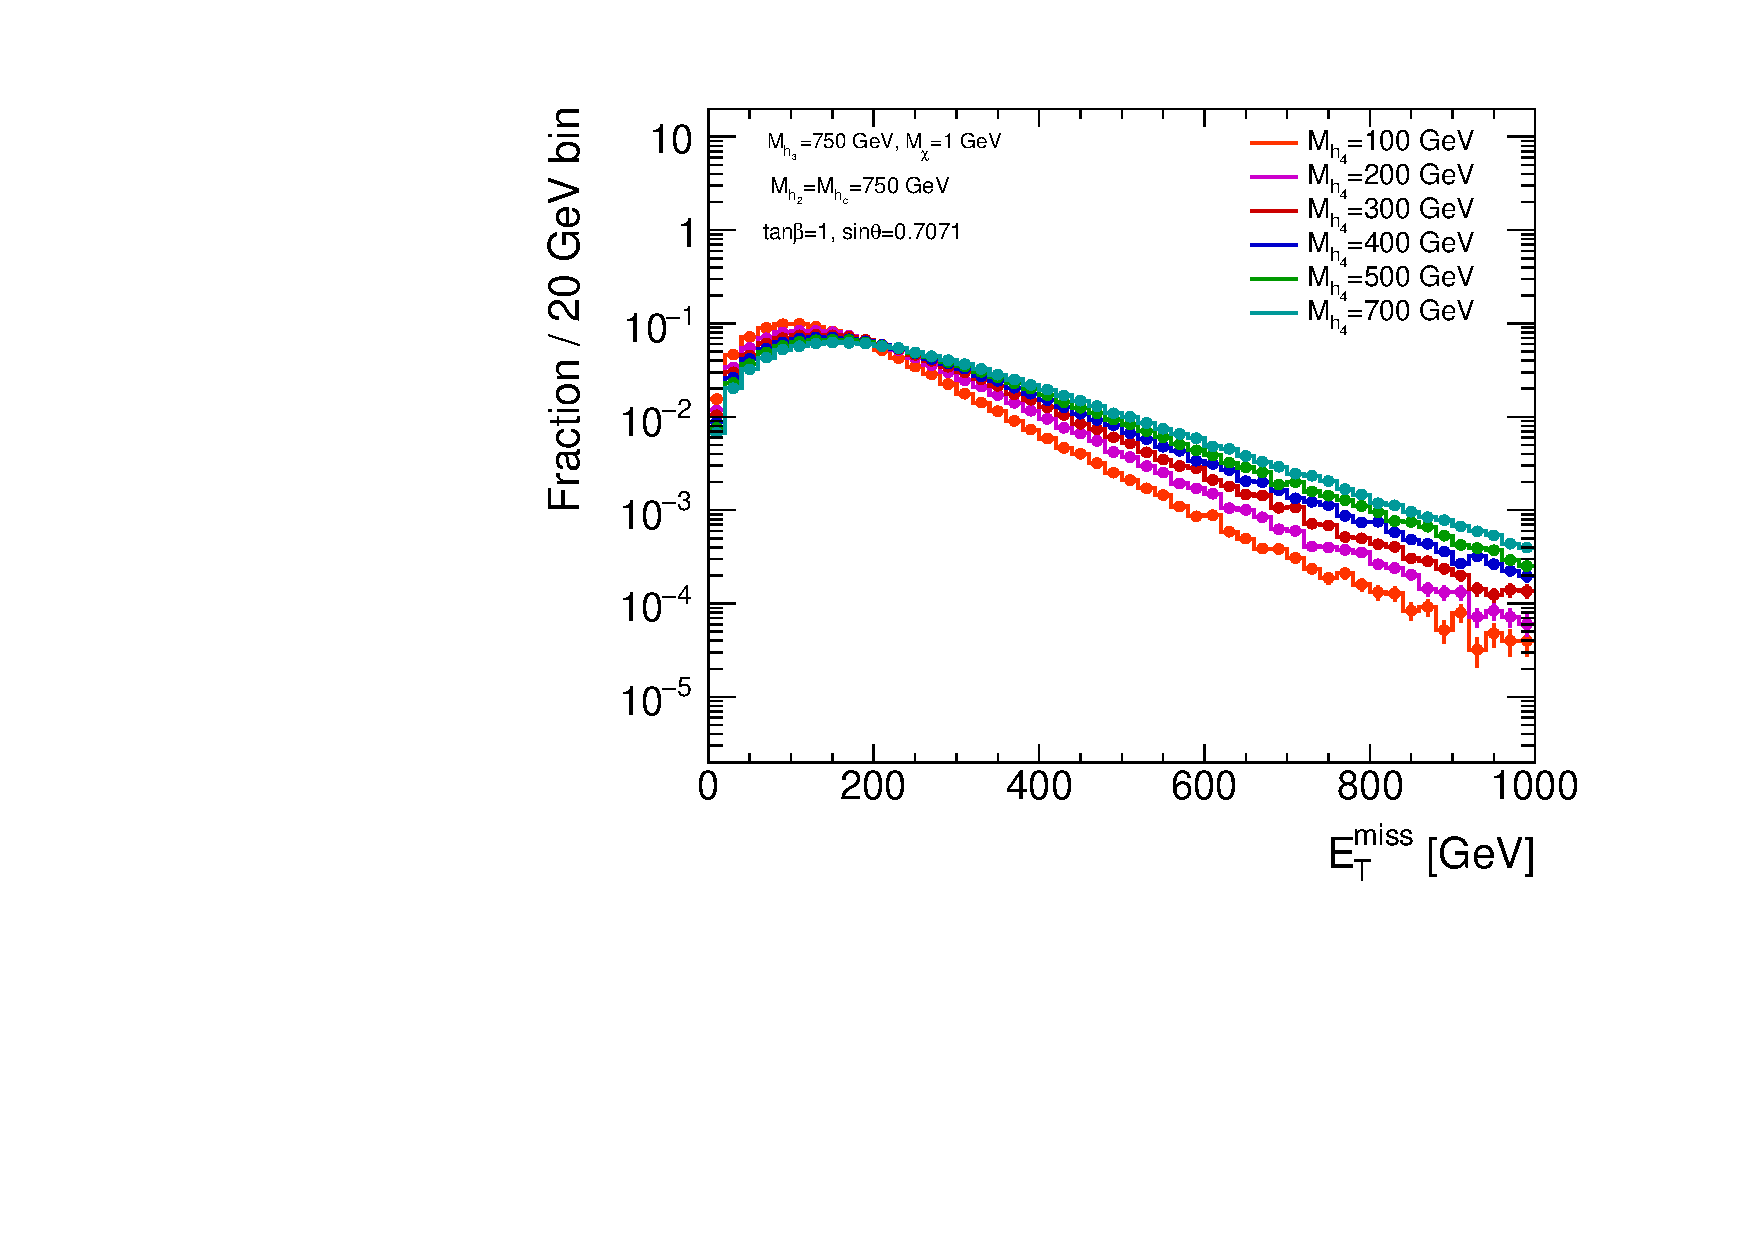
\includegraphics[width=\textwidth]{texinputs/04_grid/figures/DMHF/benchmarking/MDM_1_MA_750_sinp_0.7071_tanb_1.0_SCAN_Ma/metlog.pdf}
    \caption{$E_{T}^{miss}$}
  \end{subfigure}
  \begin{subfigure}[b]{0.49\textwidth}
    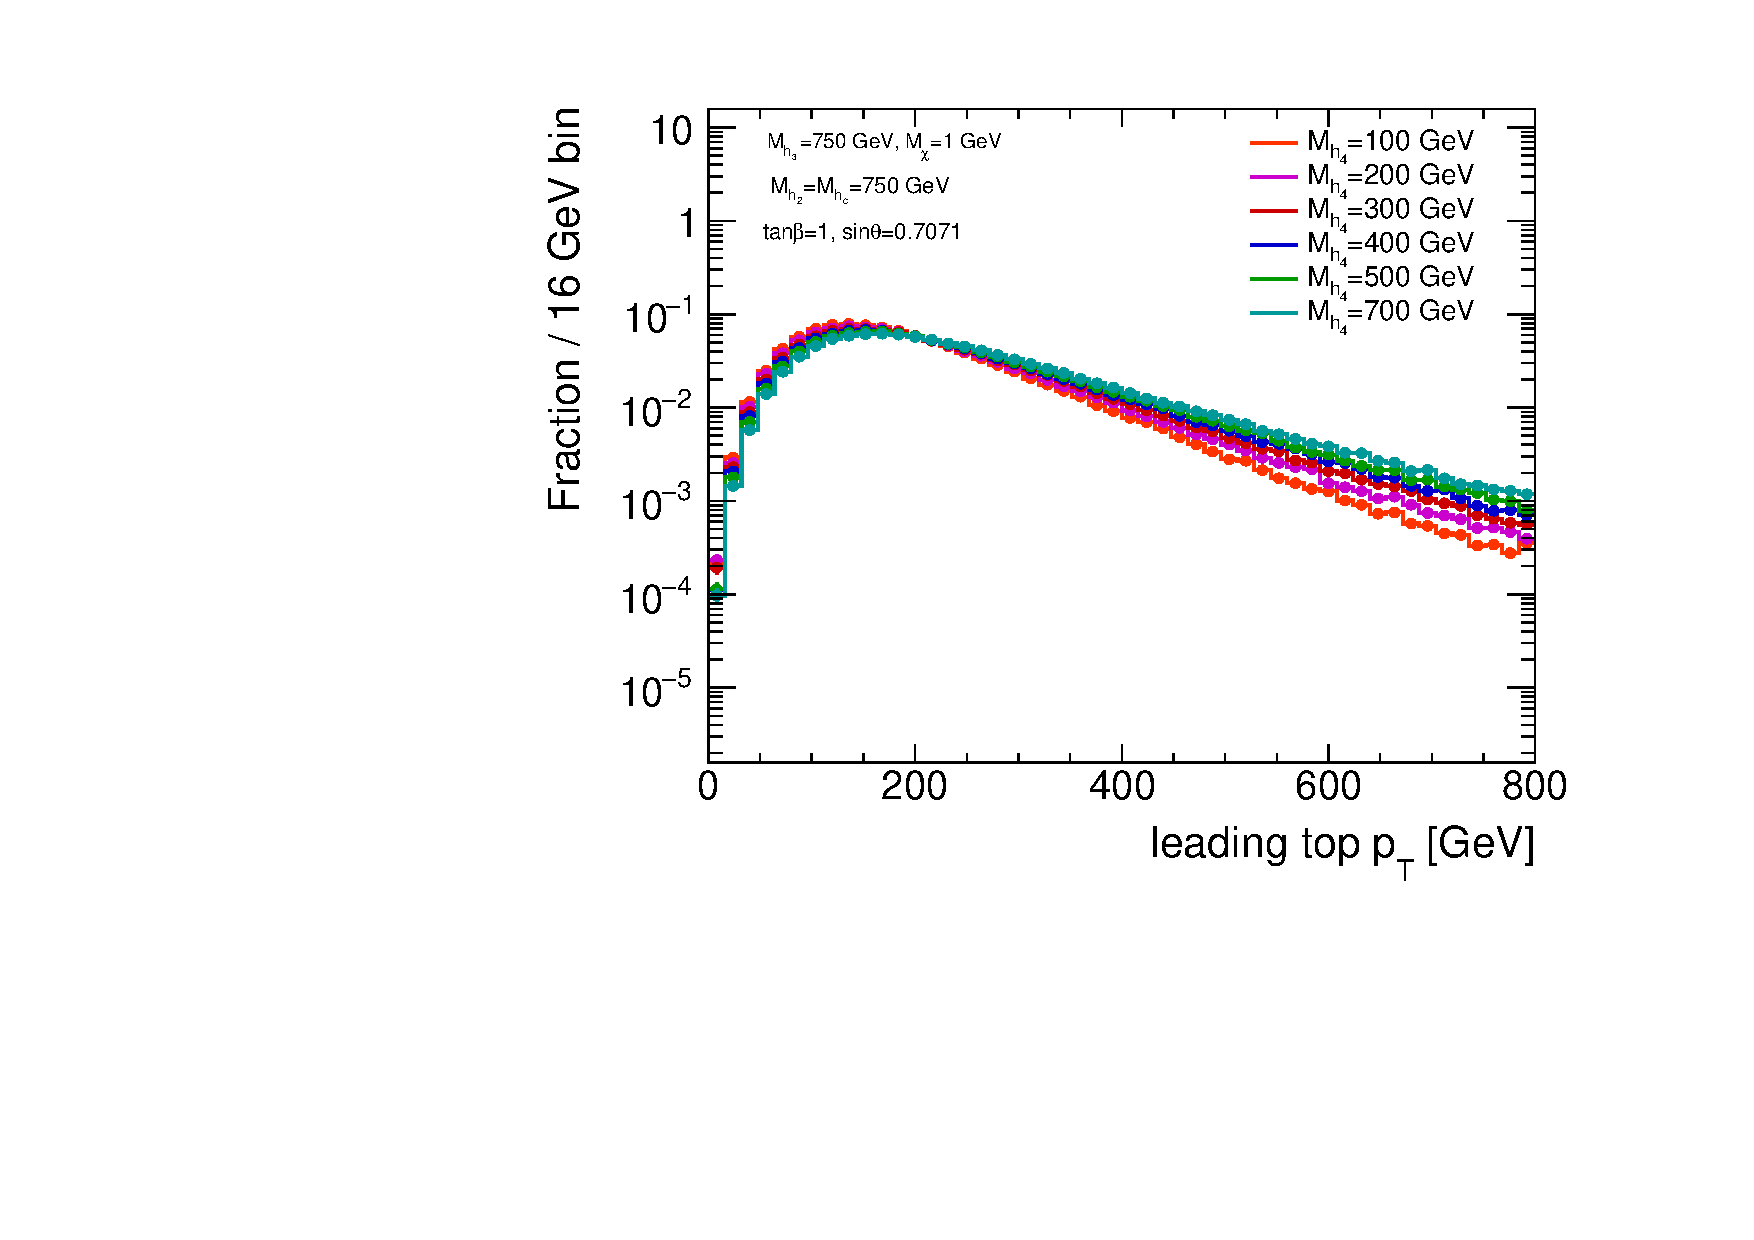
\includegraphics[width=\textwidth]{texinputs/04_grid/figures/DMHF/benchmarking/MDM_1_MA_750_sinp_0.7071_tanb_1.0_SCAN_Ma/top1ptlog.pdf}
    \caption{Leading top $p_{T}$}
  \end{subfigure} \\
  \begin{subfigure}[b]{0.49\textwidth}
    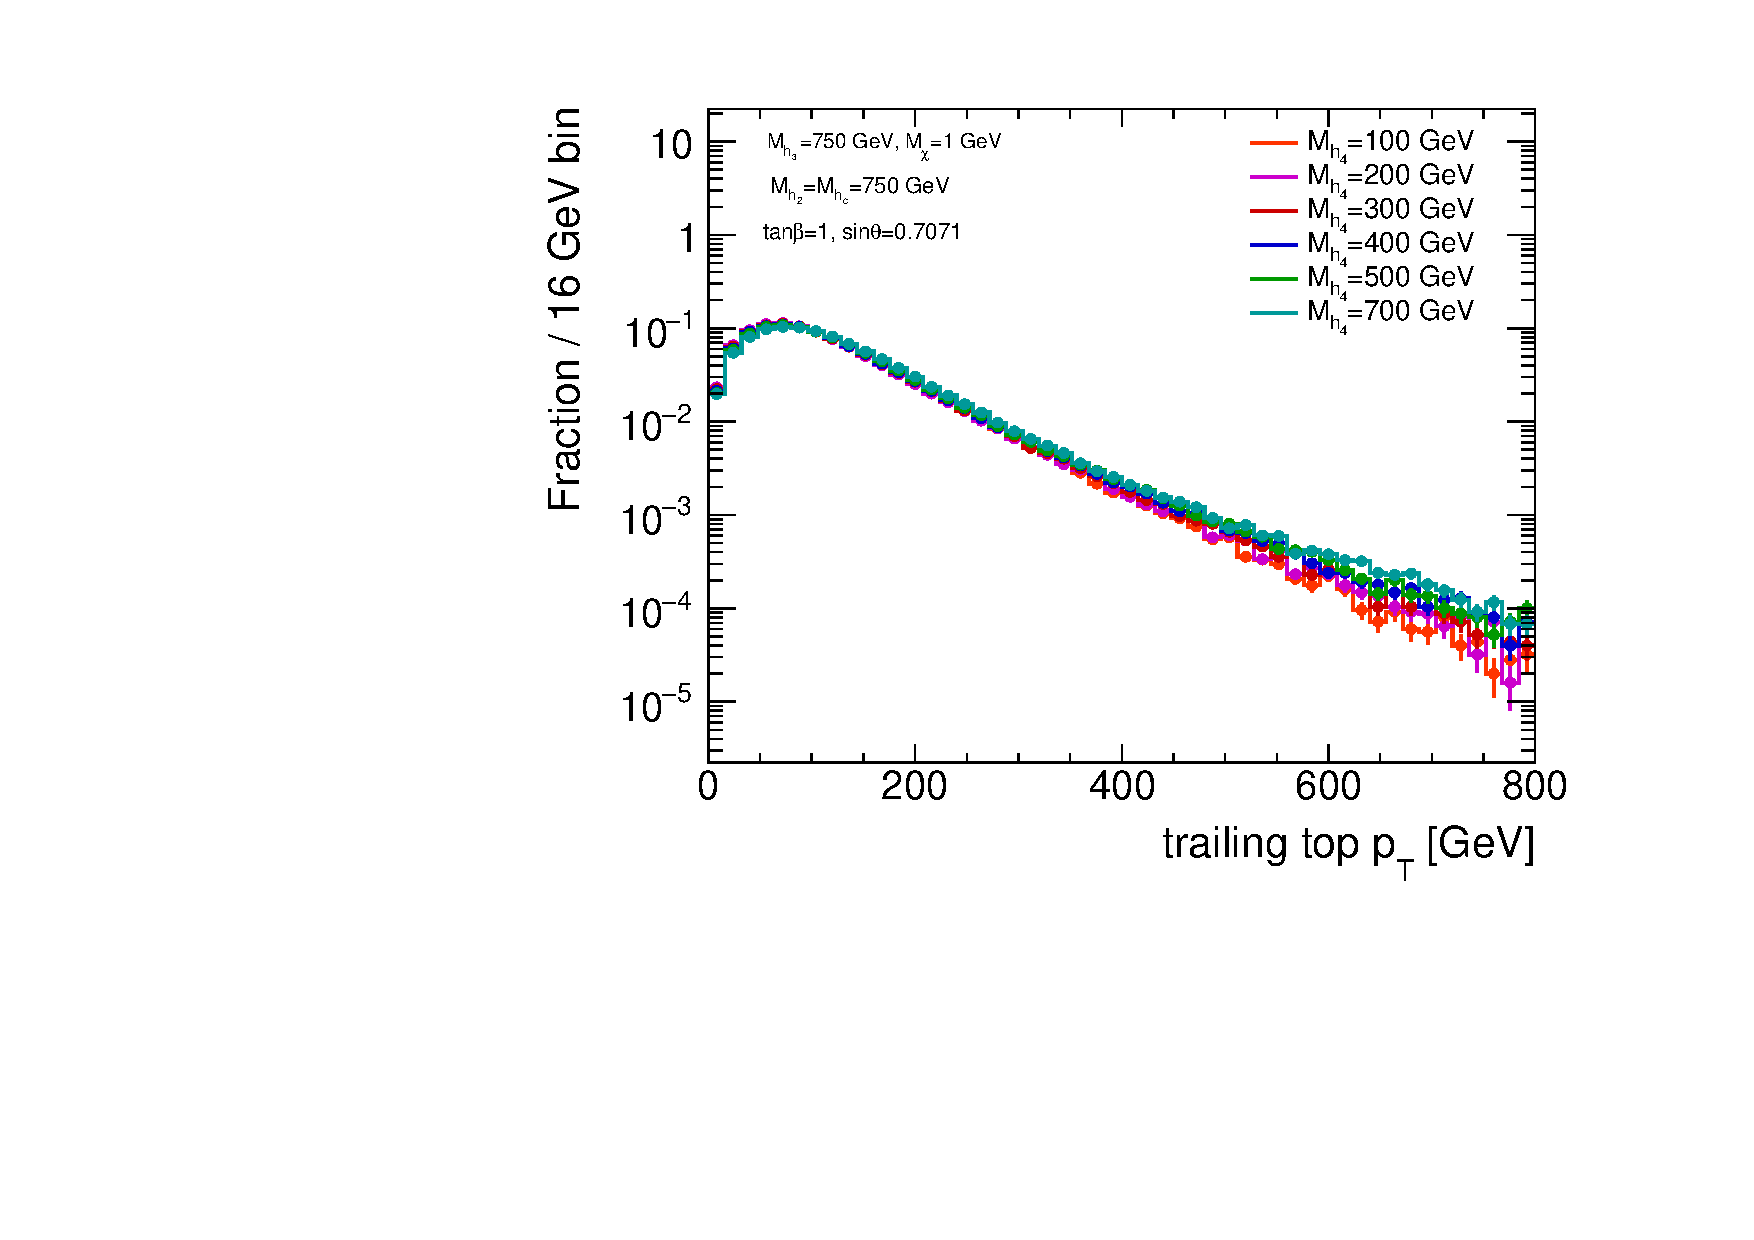
\includegraphics[width=\textwidth]{texinputs/04_grid/figures/DMHF/benchmarking/MDM_1_MA_750_sinp_0.7071_tanb_1.0_SCAN_Ma/top2ptlog.pdf}
    \caption{Trailing top $p_{T}$}
  \end{subfigure}
  \caption{The $E_{T}^{miss}$, leading and trailing top $p_{T}$ distributions for inclusive $t\bar{t}+\chi\bar{\chi}$ production for various values of $\mathrm{M_a}$, with $\mathrm{M_A}=750$ GeV, $\mathrm{M_H}=\mathrm{M_{H^{\pm}}}=750$ GeV, $\tan\beta=1$, and $\sin\theta=0.7071$.}
  \label{fig:kin_Ma}
\end{figure}

\begin{figure}
  \centering
  \begin{subfigure}[b]{0.49\textwidth}
    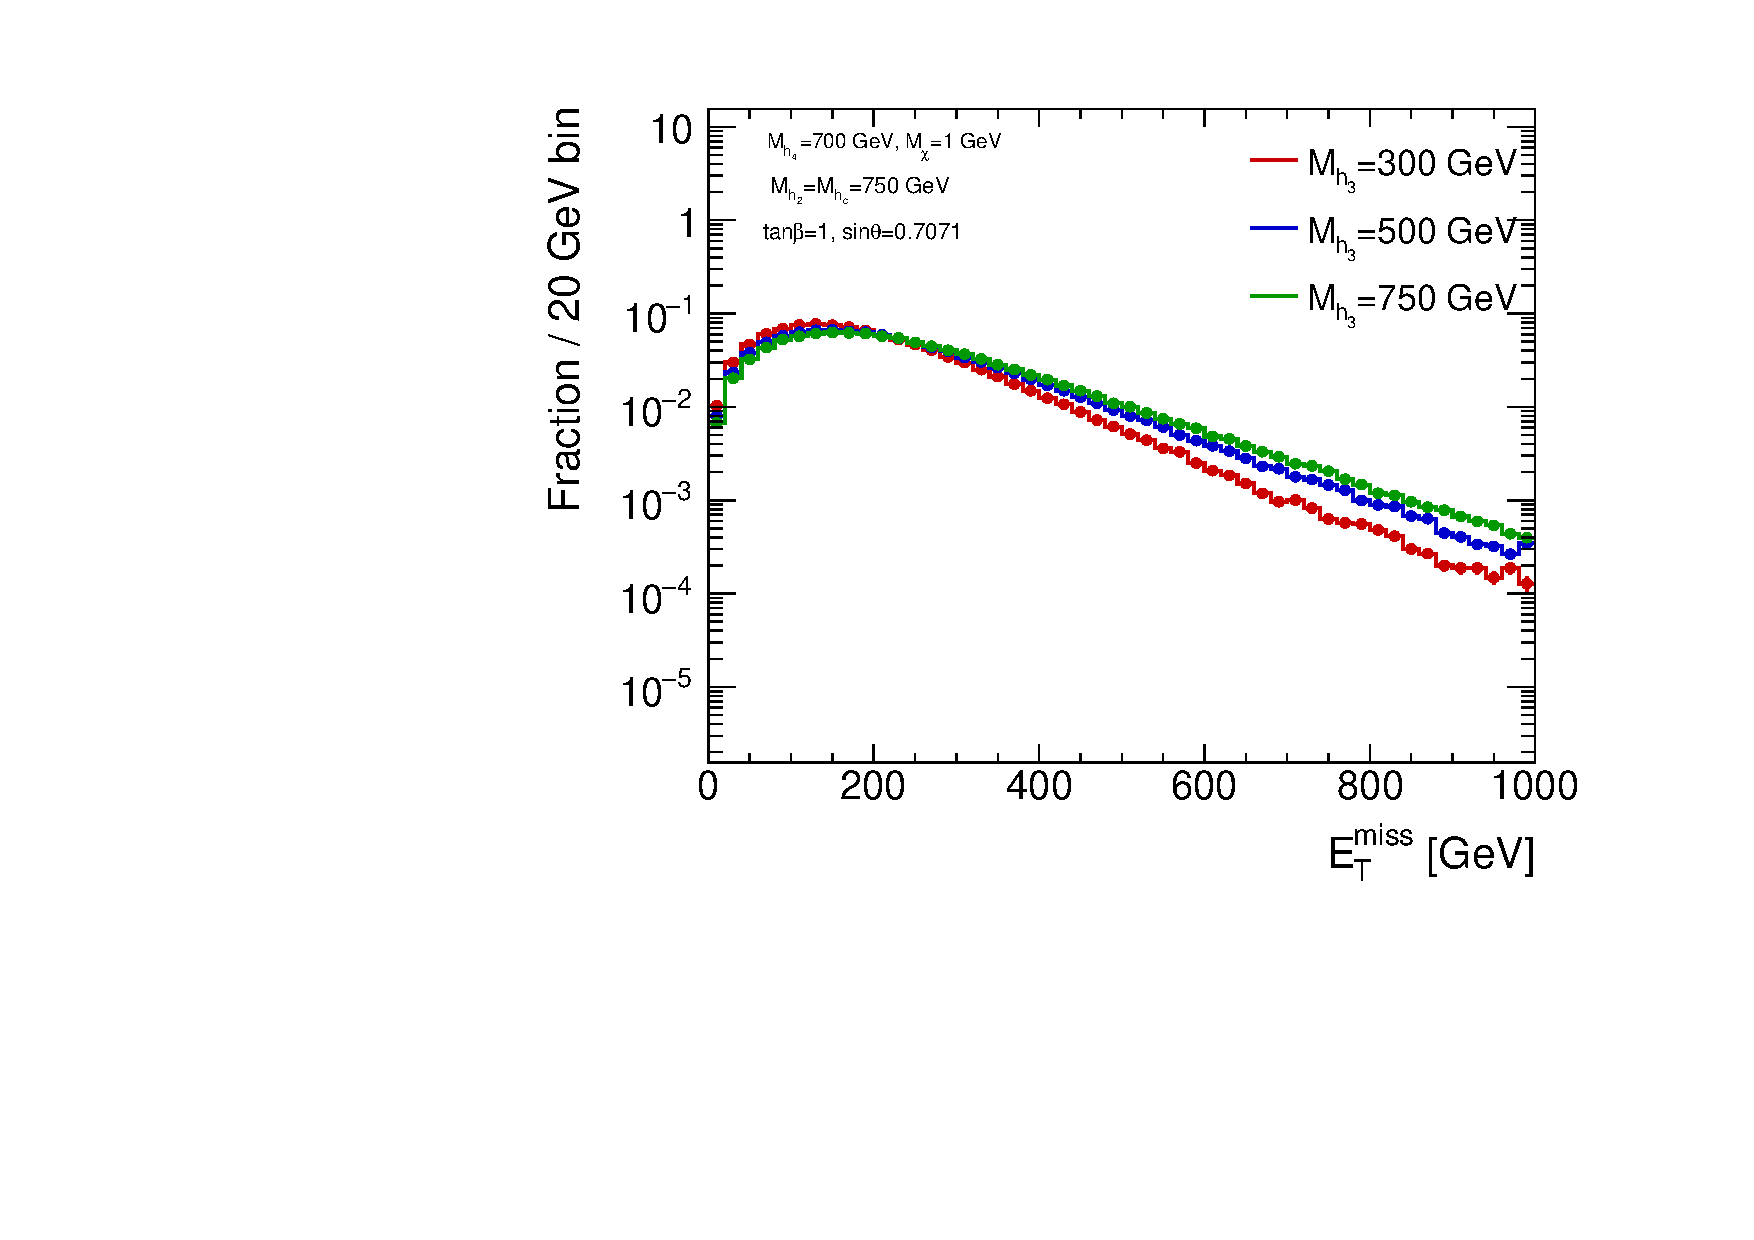
\includegraphics[width=\textwidth]{texinputs/04_grid/figures/DMHF/benchmarking/MDM_1_Ma_700_sinp_0.7071_tanb_1.0_SCAN_MA/metlog.pdf}
    \caption{$E_{T}^{miss}$}
  \end{subfigure}
  \begin{subfigure}[b]{0.49\textwidth}
    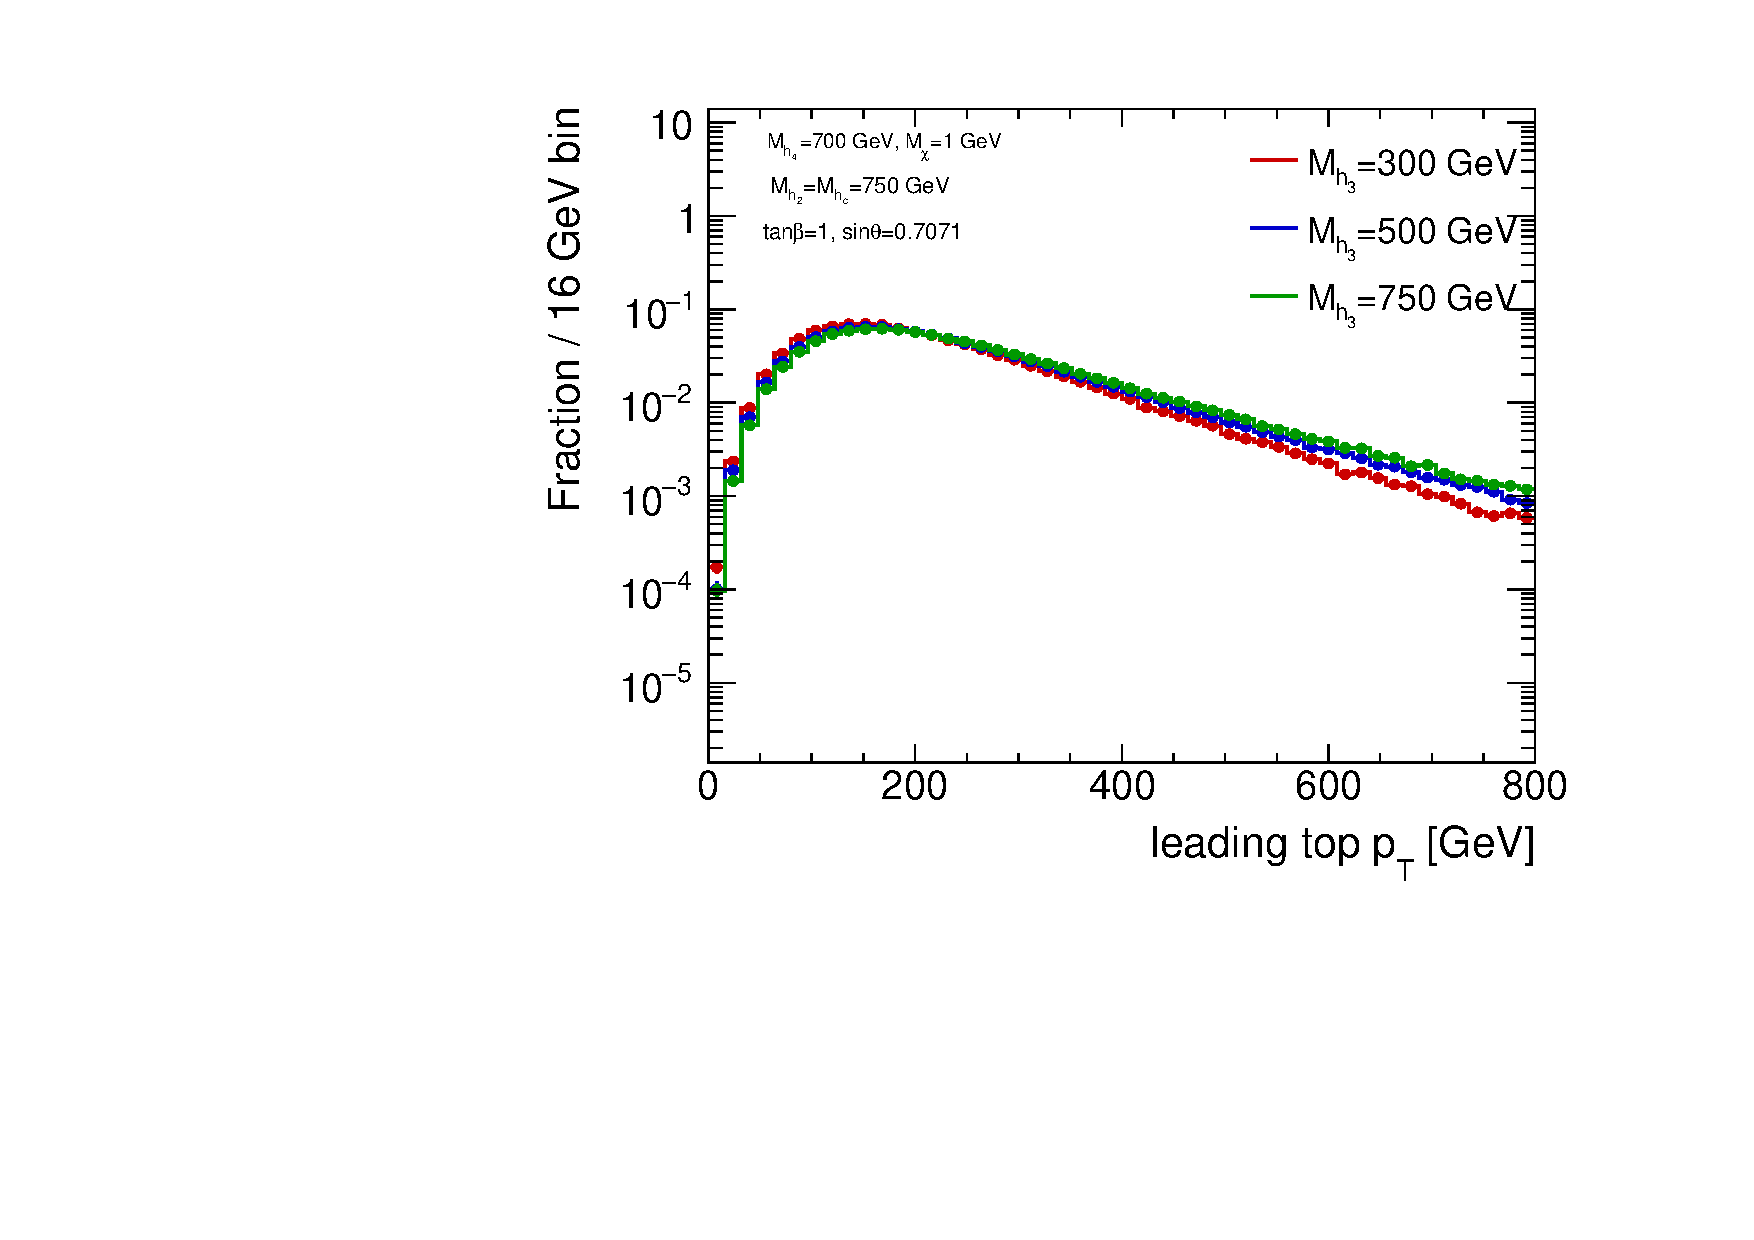
\includegraphics[width=\textwidth]{texinputs/04_grid/figures/DMHF/benchmarking/MDM_1_Ma_700_sinp_0.7071_tanb_1.0_SCAN_MA/top1ptlog.pdf}
    \caption{Leading top $p_{T}$}
  \end{subfigure} \\
  \begin{subfigure}[b]{0.49\textwidth}
    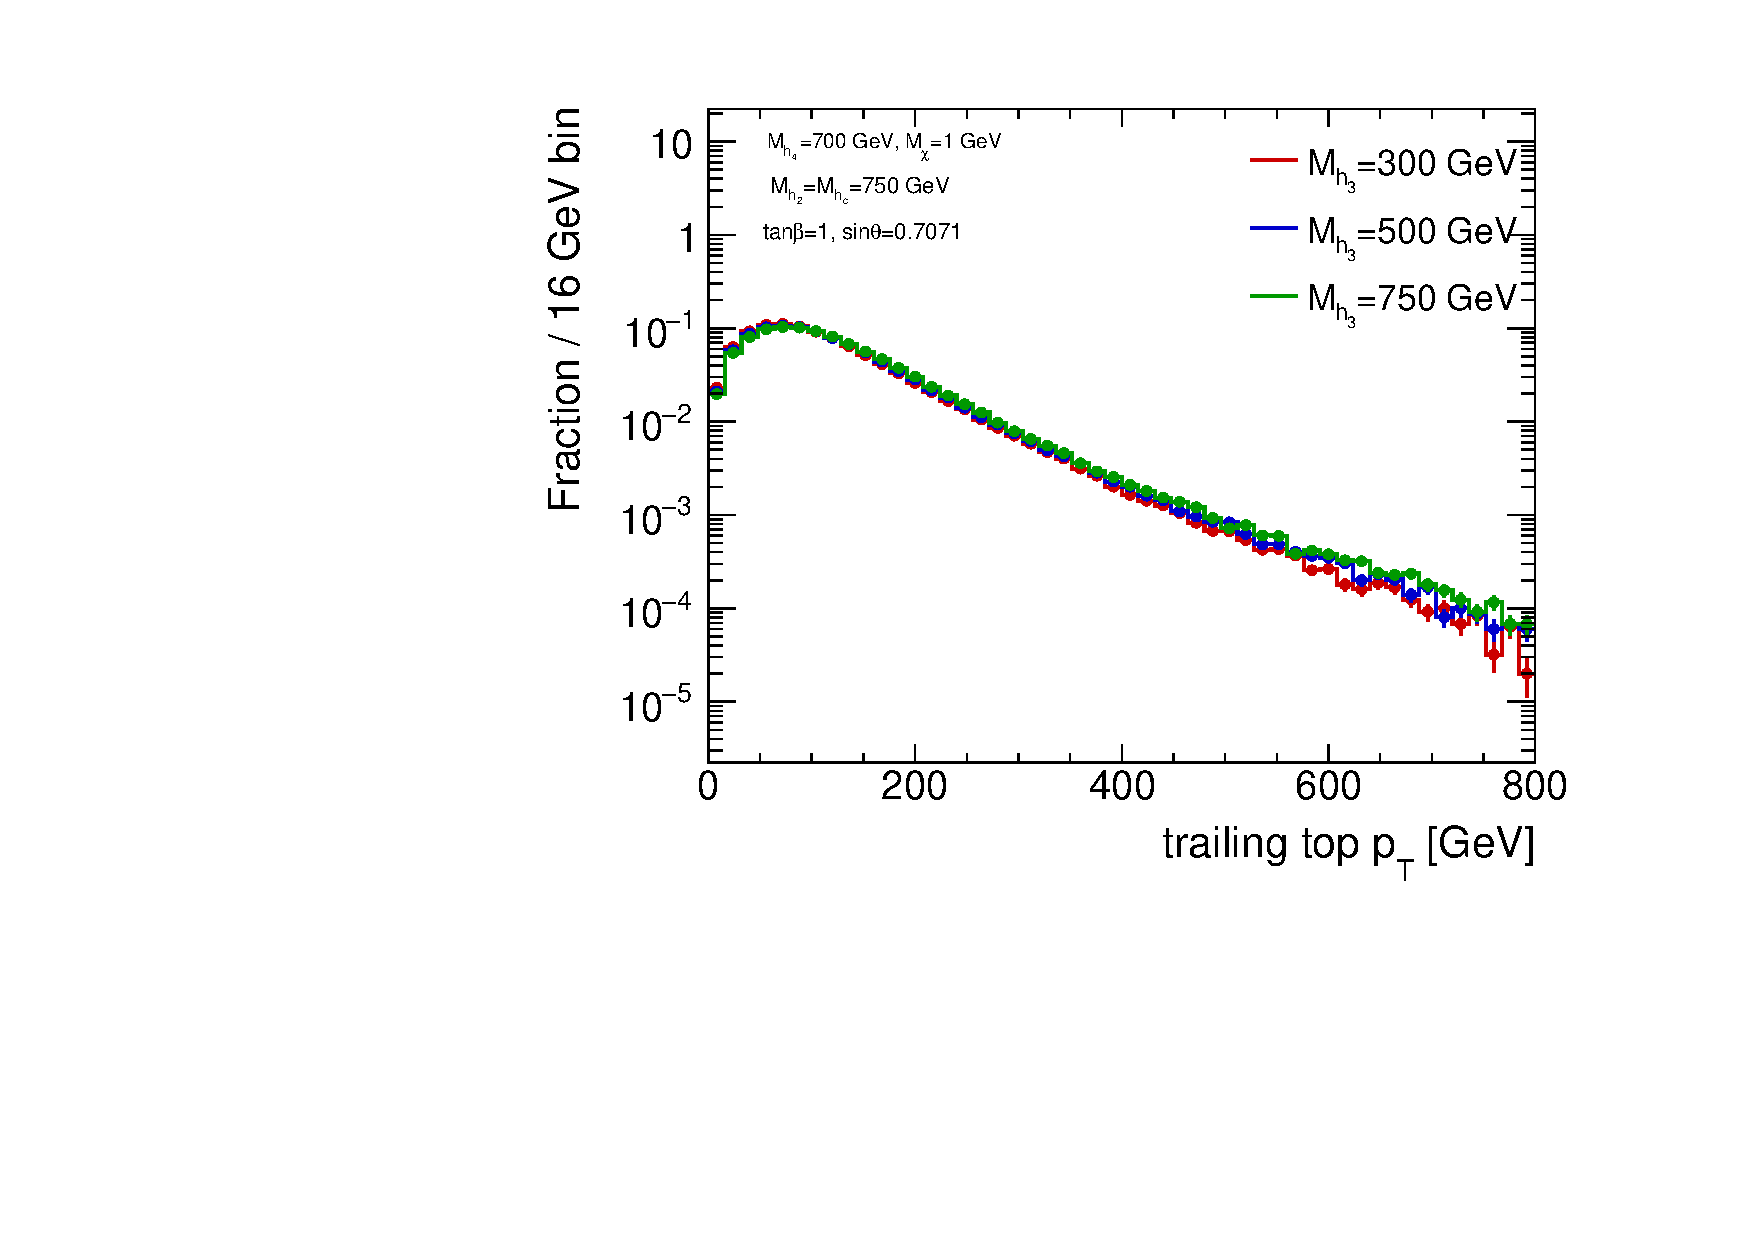
\includegraphics[width=\textwidth]{texinputs/04_grid/figures/DMHF/benchmarking/MDM_1_Ma_700_sinp_0.7071_tanb_1.0_SCAN_MA/top2ptlog.pdf}
    \caption{Trailing top $p_{T}$}
  \end{subfigure}
  \caption{The $E_{T}^{miss}$, leading and trailing top $p_{T}$ distributions for inclusive $t\bar{t}+\chi\bar{\chi}$ production for various values of $\mathrm{M_A}$, with $\mathrm{M_a}=700$ GeV, $\mathrm{M_H}=\mathrm{M_{H^{\pm}}}=750$ GeV, $\tan\beta=1$, and $\sin\theta=0.7071$.}
  \label{fig:kin_MA}
\end{figure}

Since the shape of the $\MET$ distribution affects the design of experimental searches, and to a large extent their sensitivity, it is desirable to scan the $\mA$ and $\ma$ parameter space. 

%In conclusion, the $\mA$ and $\ma$ parameters strongly affect the sensitivity of a search for the \hdma model using the \monohbb signature because they determine the location of the Jacobian peak in the \met distribution. Therefore, one of the proposed parameter scans for the \hdma model is in the ($\ma$,$\mA$) plane.

\begin{figure}%[!htpb]
\centering
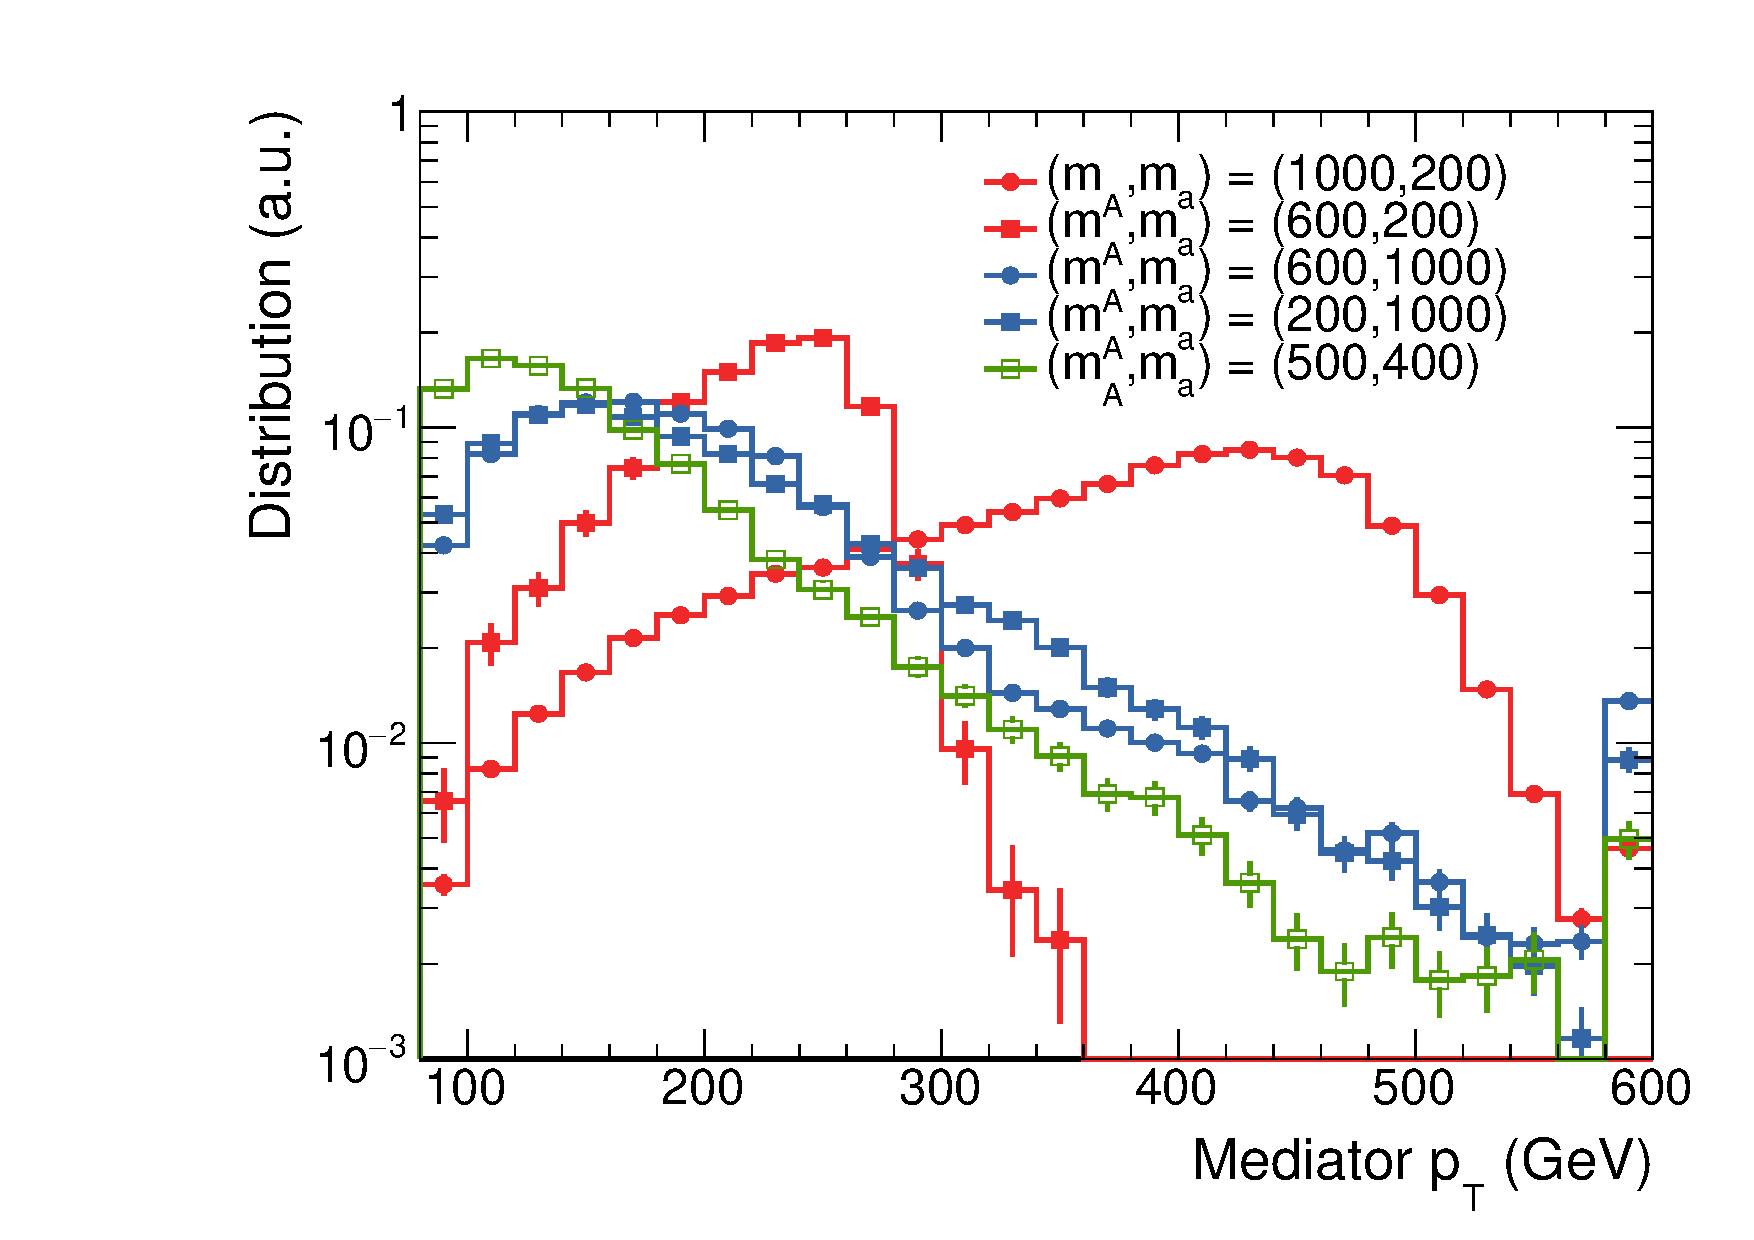
\includegraphics[width=0.45\textwidth]{texinputs/04_grid/figures/monoz/leptonic/dmwg-final_h_pt_med_dm.pdf}
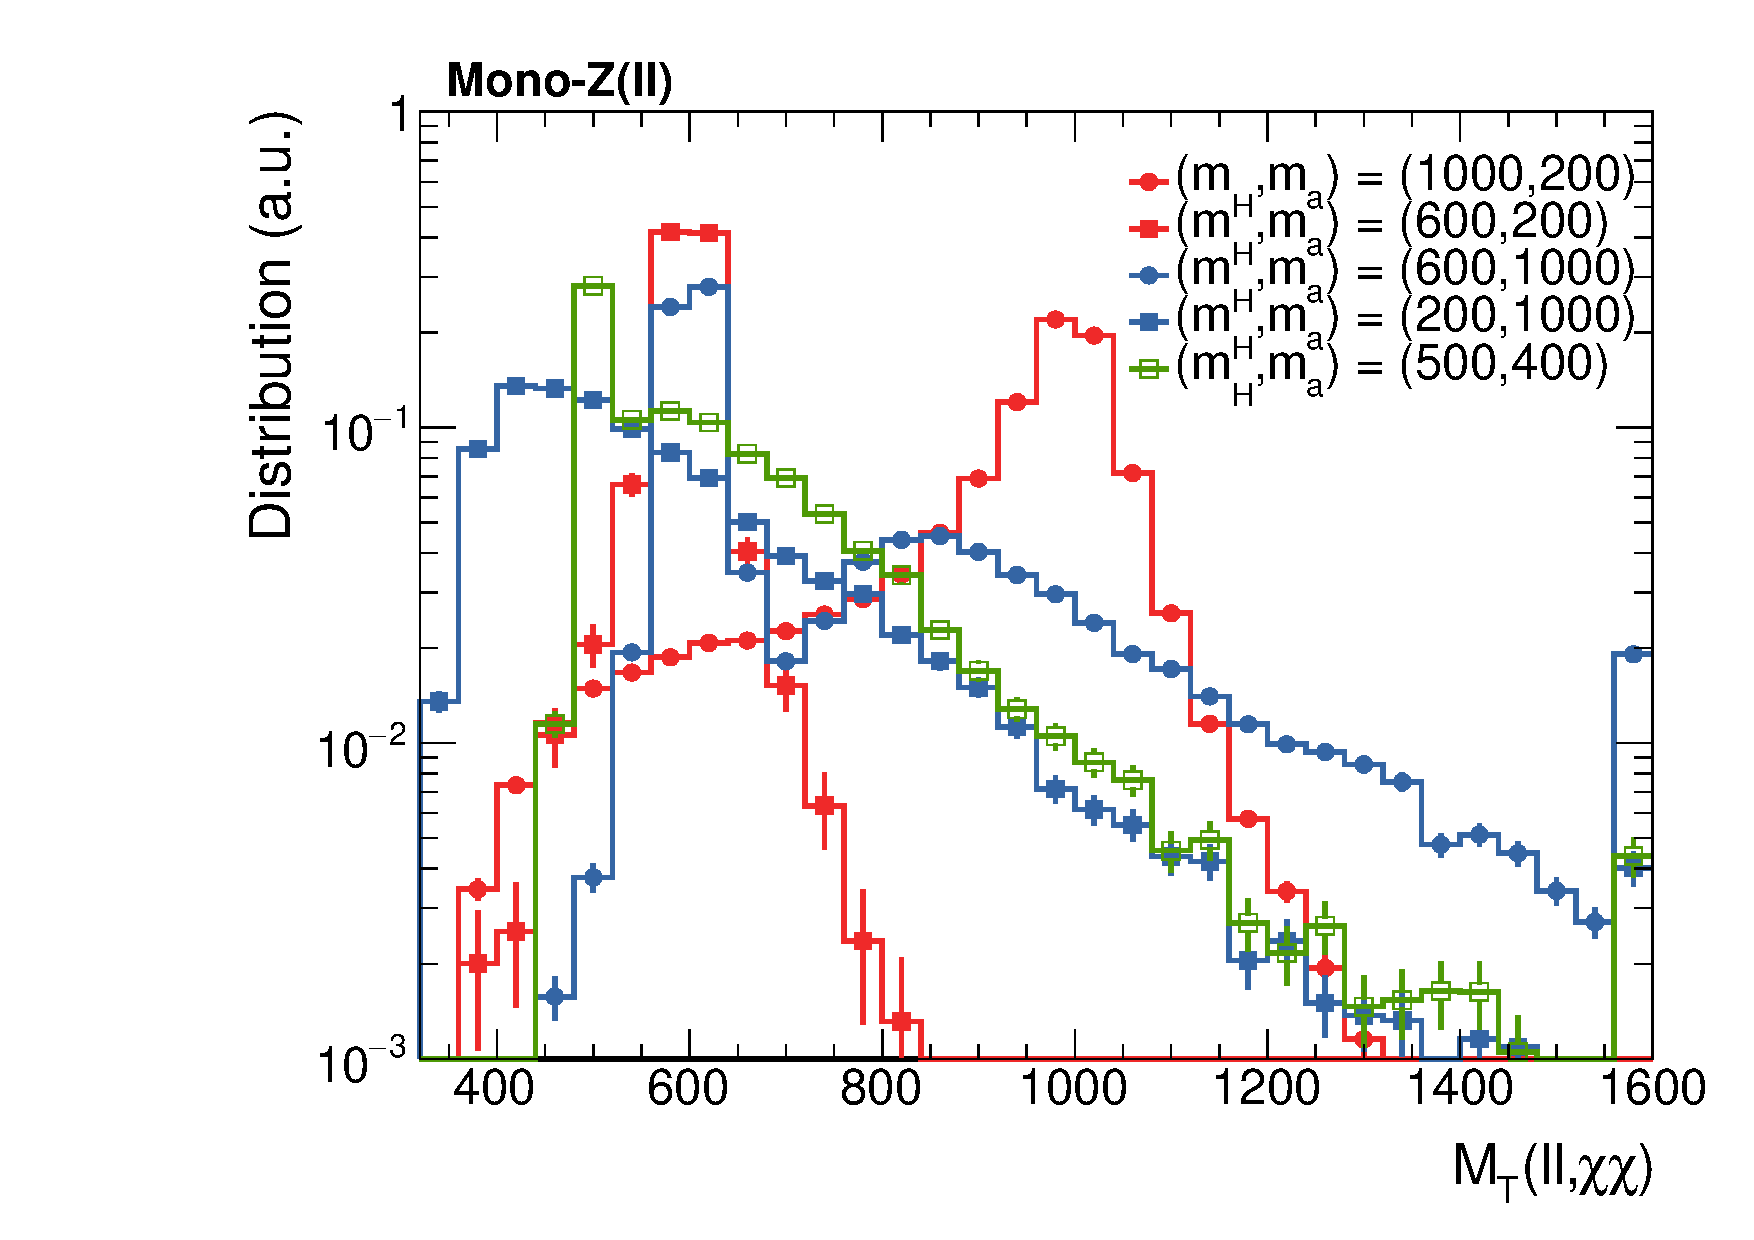
\includegraphics[width=0.45\textwidth]{texinputs/04_grid/figures/monoz/leptonic/dmwg-final_h_mt_total.pdf}
\caption{\MET and  $\MT$ distributions after the full selection of Z(lep)+\MET search. Both distributions show a peaked structure around $\mA$ in the $\mA > \ma$ regime, reflecting the resonant production of $A$.}
\label{fig:monoz_kin_final}
\end{figure}

As an additional remark on the design of these searches, the distributions of the $\MET$ and $\MT$ variables after final selection are shown in ~\autoref{fig:monoz_kin_final} for the Z+\MET searches. Traditionally, these searches have relied on the $\MET$ distribution for signal extraction. While the presence of the Jacobian peak structure in the distribution facilitates signal-background separation, it may be beneficial to also consider the $\MT$ distribution. Although only transverse information is available, the resonant structure of the signal is significantly enhanced in the $\MT$ variable, which may enhance the sensitivity of a specialized search strategy exploiting this characteristic.
In the region of inverted mass hierarchy $\mA < \ma$, the \MET spectrum is less structured and does not fall off as steeply towards higher values. For a small mass splitting of $\ma-\mA\approx M_{Z}$, the spectrum is shifted to much lower values of \MET. 
The $\MT$ distribution allows to access the resonant nature of the process. Clear mass peaks are present for the normal mass hierarchy. In the inverted region, the MT distribution is more sensitive to the mass difference $\ma-\mA$ than the \MET distribution, allowing to differentiate between signal hypotheses that give near-identical \MET distributions.

\subsubsection{Masses of the heavy neutral and charged scalar Higgs bosons $H, H^{\pm}$ ($\mH$, $m_{H^{\pm}}$)}

The mass of the heavy neutral scalar Higgs boson $H$ has an indirect effect on the rate and kinematics of the signal. 
This is caused by the dependence of the coupling strengths and thus decay widths of  the pseudoscalars $A$ and $a$ on  $\mH$~\cite{Bauer:2017ota}. 
Therefore, a change of $\mH$ can affect the relative contribution of resonant versus non-resonant signal processes, as illustrated in \autoref{fig:monoHbb_mH_scan_met}.

The choice $\mH = \mA$ results in a detectable total cross section for many signal points and a dominant contribution of the resonant signal process. 
%Do we show this somewhere?
This choice allows us to test diverse $\MET$ distributions and results in about equal contributions to the sensitivity through the \monoz and \monoh signatures, highlighting their complementarity. For this reason $\mH = \mA$ is adopted for all scans. For simplicity, the neutral scalar $H^{\pm}$ is assumed to be mass-degenerate to $H$, as it does not affect the \hdma model kinematics.

%as demonstrated in \autoref{fig:monoHbb_mA_scan_met} and \autoref{fig:monoHbb_ma_scan_met}

\begin{figure}[!htbp]
	\centering

%	\begin{subfigure}[t]{0.75\textwidth}
%	\centering
	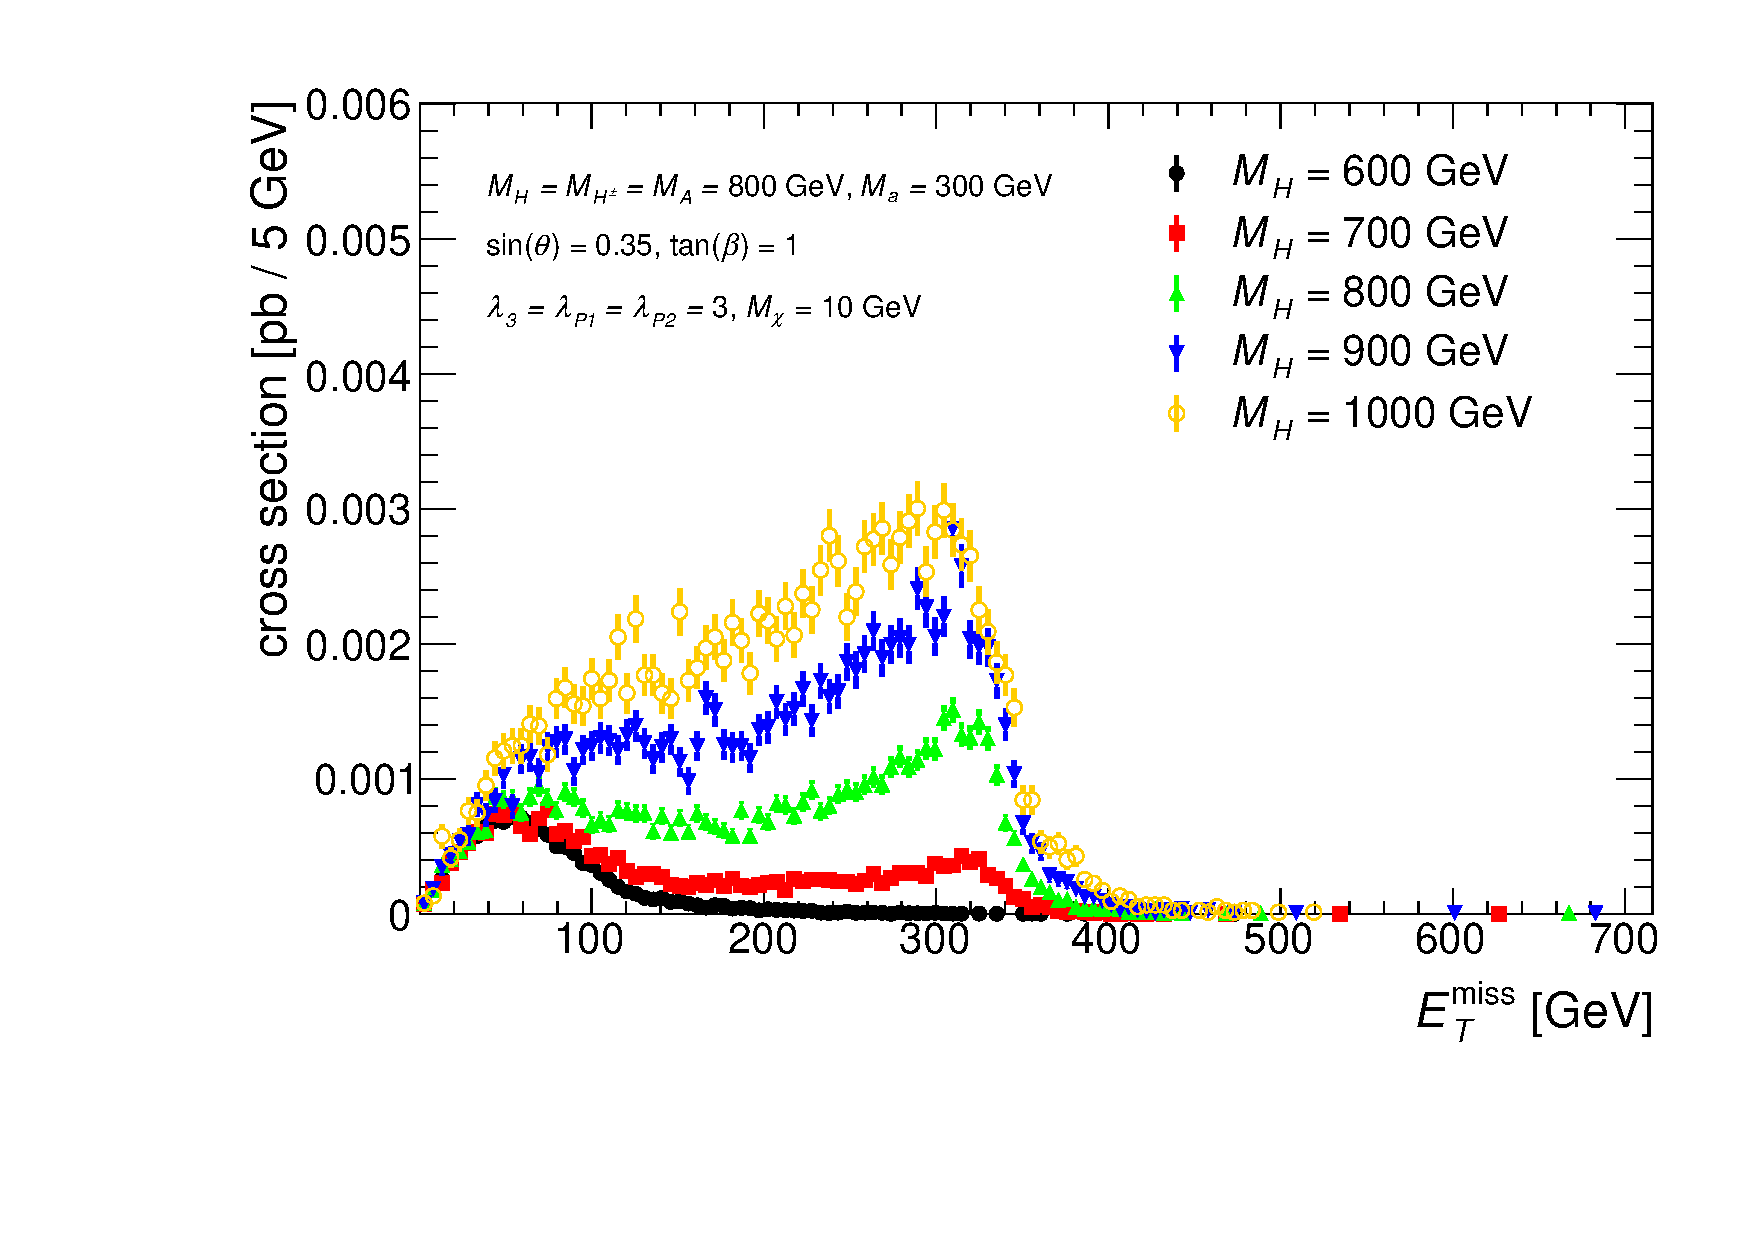
\includegraphics[width=0.75\textwidth]{texinputs/04_grid/figures/monoHbb_mH_scan_MET_liny.pdf}
	\caption{The \MET distribution, accounting for the production cross section, of \monohbb signal events for five representative choices of $\mH = \mHc$.
	%and fixed $ \mA=800$ GeV, $\ma = 300 $ GeV,  $ \sinp = 0.35, \tanb = 1, \mDM = 10$ GeV and $ \lap1 = \lap2 = \lam3 = 3 $.
	\label{fig:monoHbb_mH_scan_met}} 
%    \end{subfigure}
     
	\caption{$\MET$ distribution in \monohbb and Z+\MET events for different $\mH$}
\end{figure}

\subsubsection{Mixing angle between the two pseudoscalars $A$ and $a$ ($\sinp$)}

The sine of the mixing angle between the two pseudoscalars $A$ and $a$, $\sinp$,affects not only the cross section, but also the shape of the \MET\ distribution in searches including a Higgs boson, as shown in \autoref{fig:monoHbb_sinp_scan_mA600_ma200_met}. 
For the resonant diagram $gg\rightarrow A \rightarrow ah \rightarrow \chi\bar{\chi}h$, the product of cross section times branching ratios  ${\cal B}(A\rightarrow ah){\cal B}(a \rightarrow \chi\bar{\chi})$ scales with $\sin^2\theta\cos^6\theta$, while for the diagram $gg\rightarrow a \rightarrow A^*h \rightarrow \chi\bar{\chi}h$, the product of cross section times branching ratios ${\cal B}(a\rightarrow Ah){\cal B}(A \rightarrow \chi\bar{\chi})$ scales with $\sin^6\theta\cos^2\theta$. 
Therefore, at small \sinp, the resonant diagram $A\rightarrow ah$ is the dominant production mode and the \MET\ distribution has a Jacobian peak following \autoref{eq:monoH_peak_met}; while at large \sinp, the $a\rightarrow A^*h$ diagram starts to dominate and produces a second peak at a lower \MET\ value.
Scans of the \sinp parameter show they have minimal effect on the kinematic distributions for searches with a Z boson (\autoref{fig:monoz_kin_sintheta}).  

\begin{figure}
  \centering
  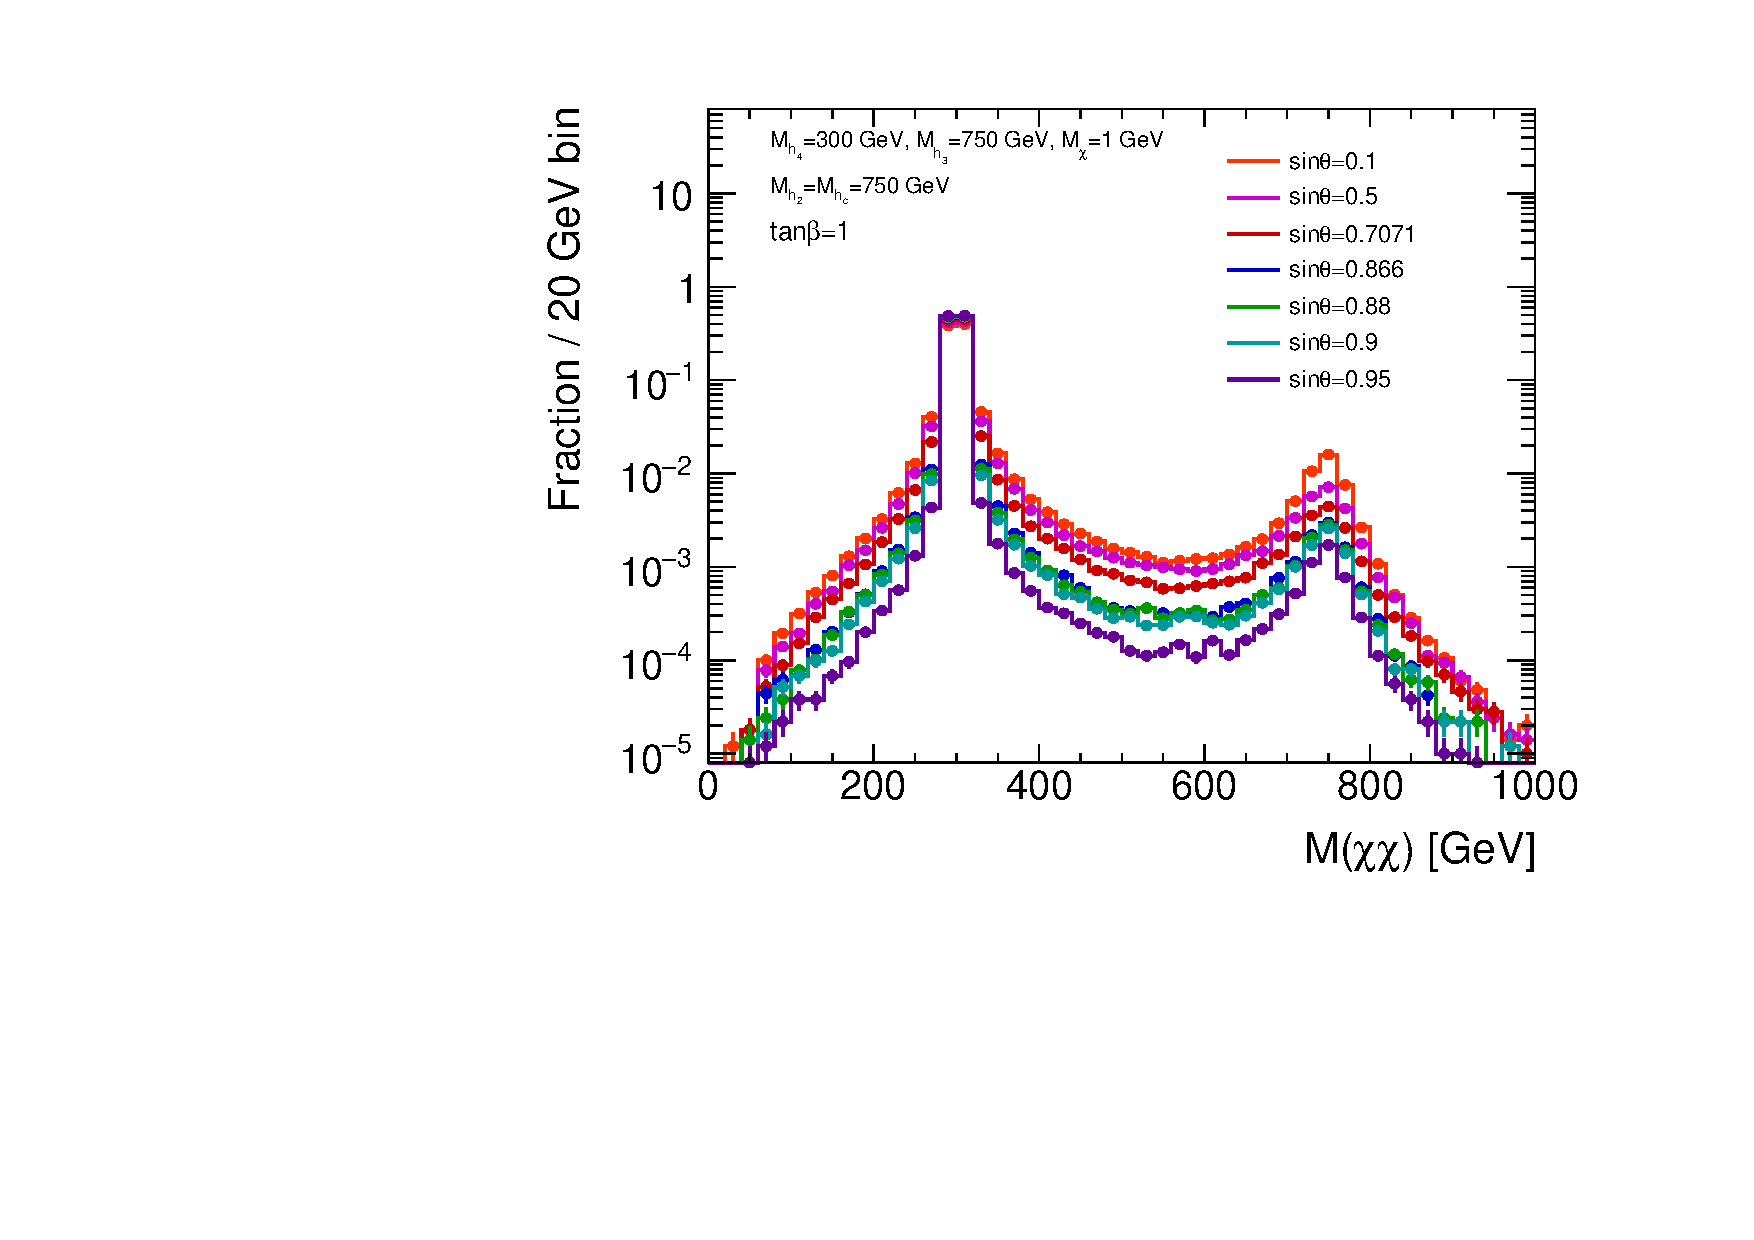
\includegraphics[width=0.6\textwidth]{texinputs/04_grid/figures/DMHF/benchmarking/MDM_1_Ma_300_MA_750_tanb_1.0_SCAN_sinp_v2/mchichi.pdf}
  \caption{The mass distribution of the $\chi \bar{\chi}$ system for various values of $\sin\theta$, with $\mathrm{M_a}=300$ GeV, $\mathrm{M_A}=750$ GeV, $\mathrm{M_H}=\mathrm{M_{H^{\pm}}}=750$ GeV, and $\tan\beta=1$.}
  \label{fig:mchichi_sinp}
\end{figure} 

\begin{figure}
  \centering
  \begin{subfigure}[b]{0.49\textwidth}
    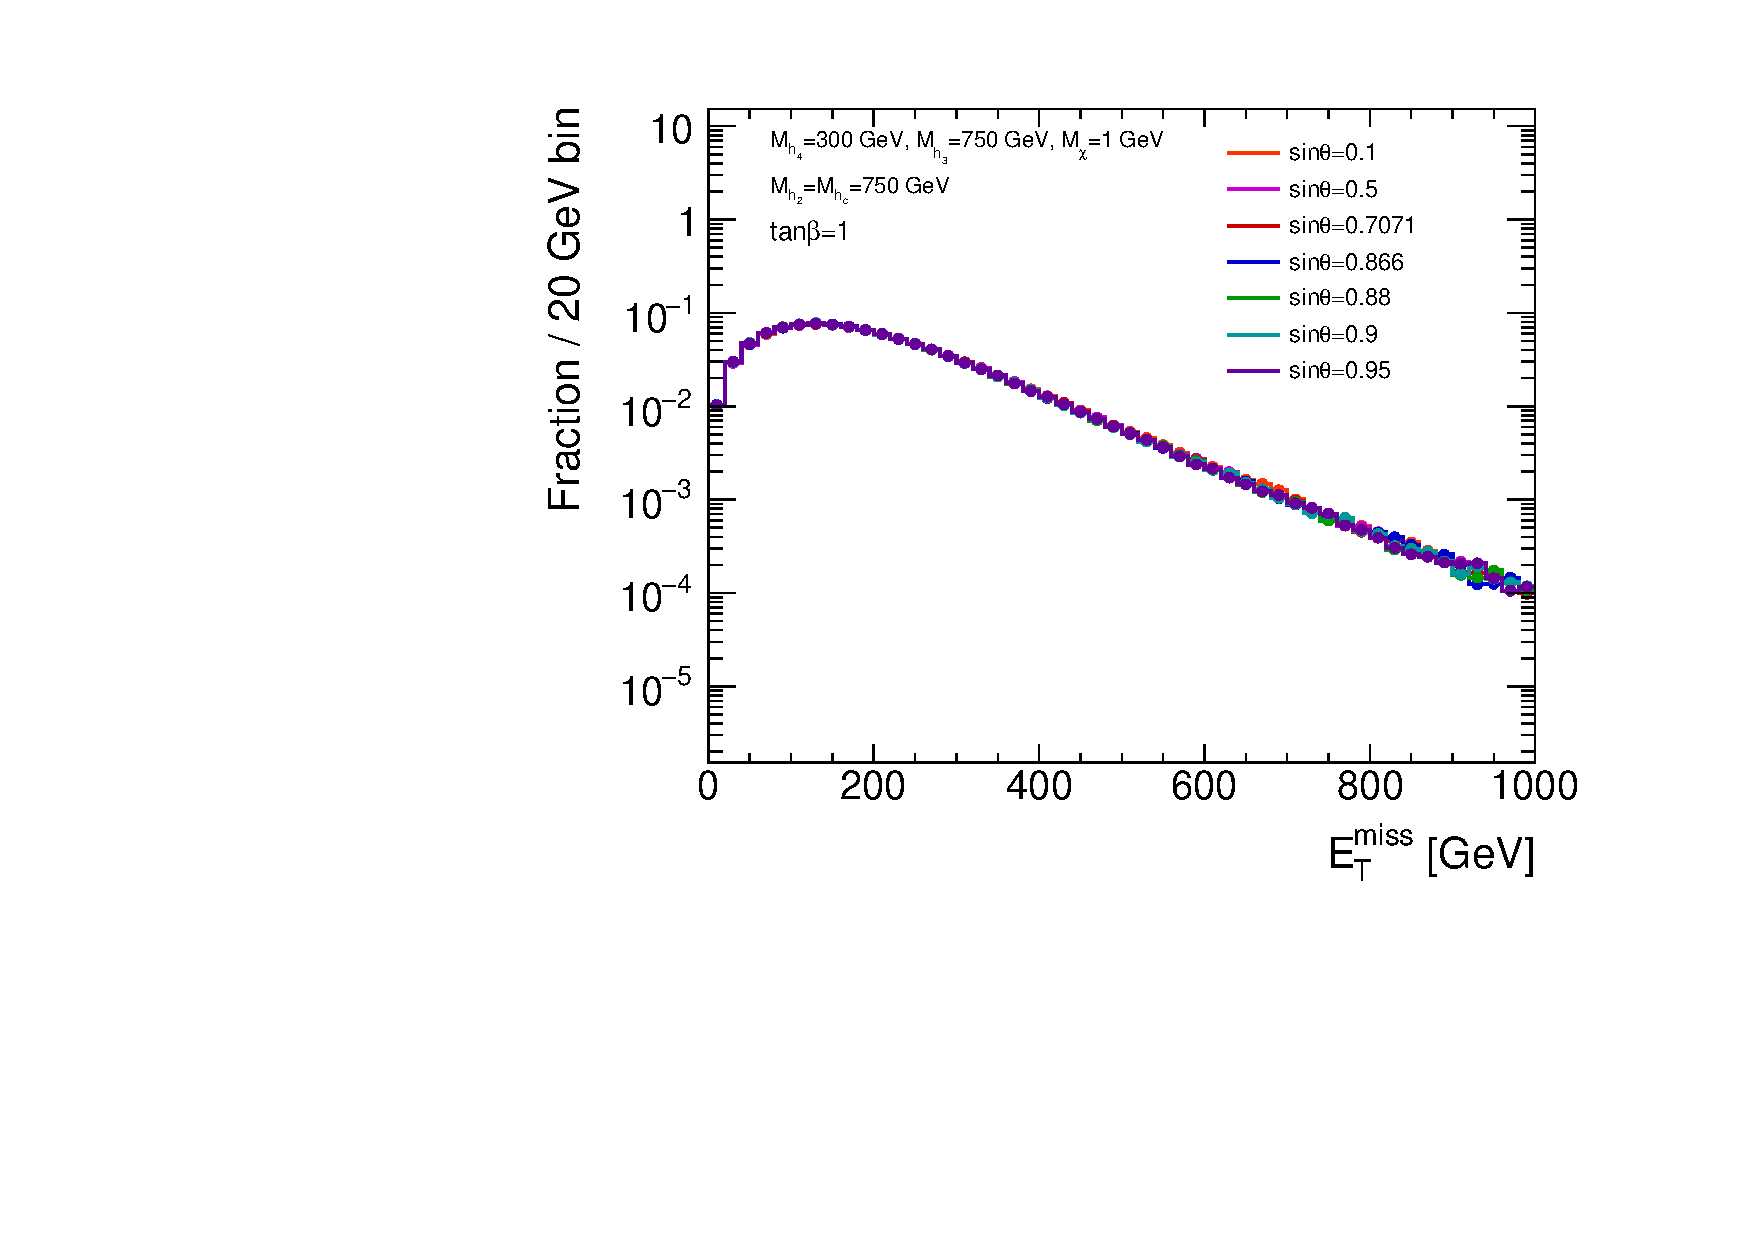
\includegraphics[width=\textwidth]{texinputs/04_grid/figures/DMHF/benchmarking/MDM_1_Ma_300_MA_750_tanb_1.0_SCAN_sinp_v2/metlog.pdf}
    \caption{$E_{T}^{miss}$}
  \end{subfigure}
  \begin{subfigure}[b]{0.49\textwidth}
    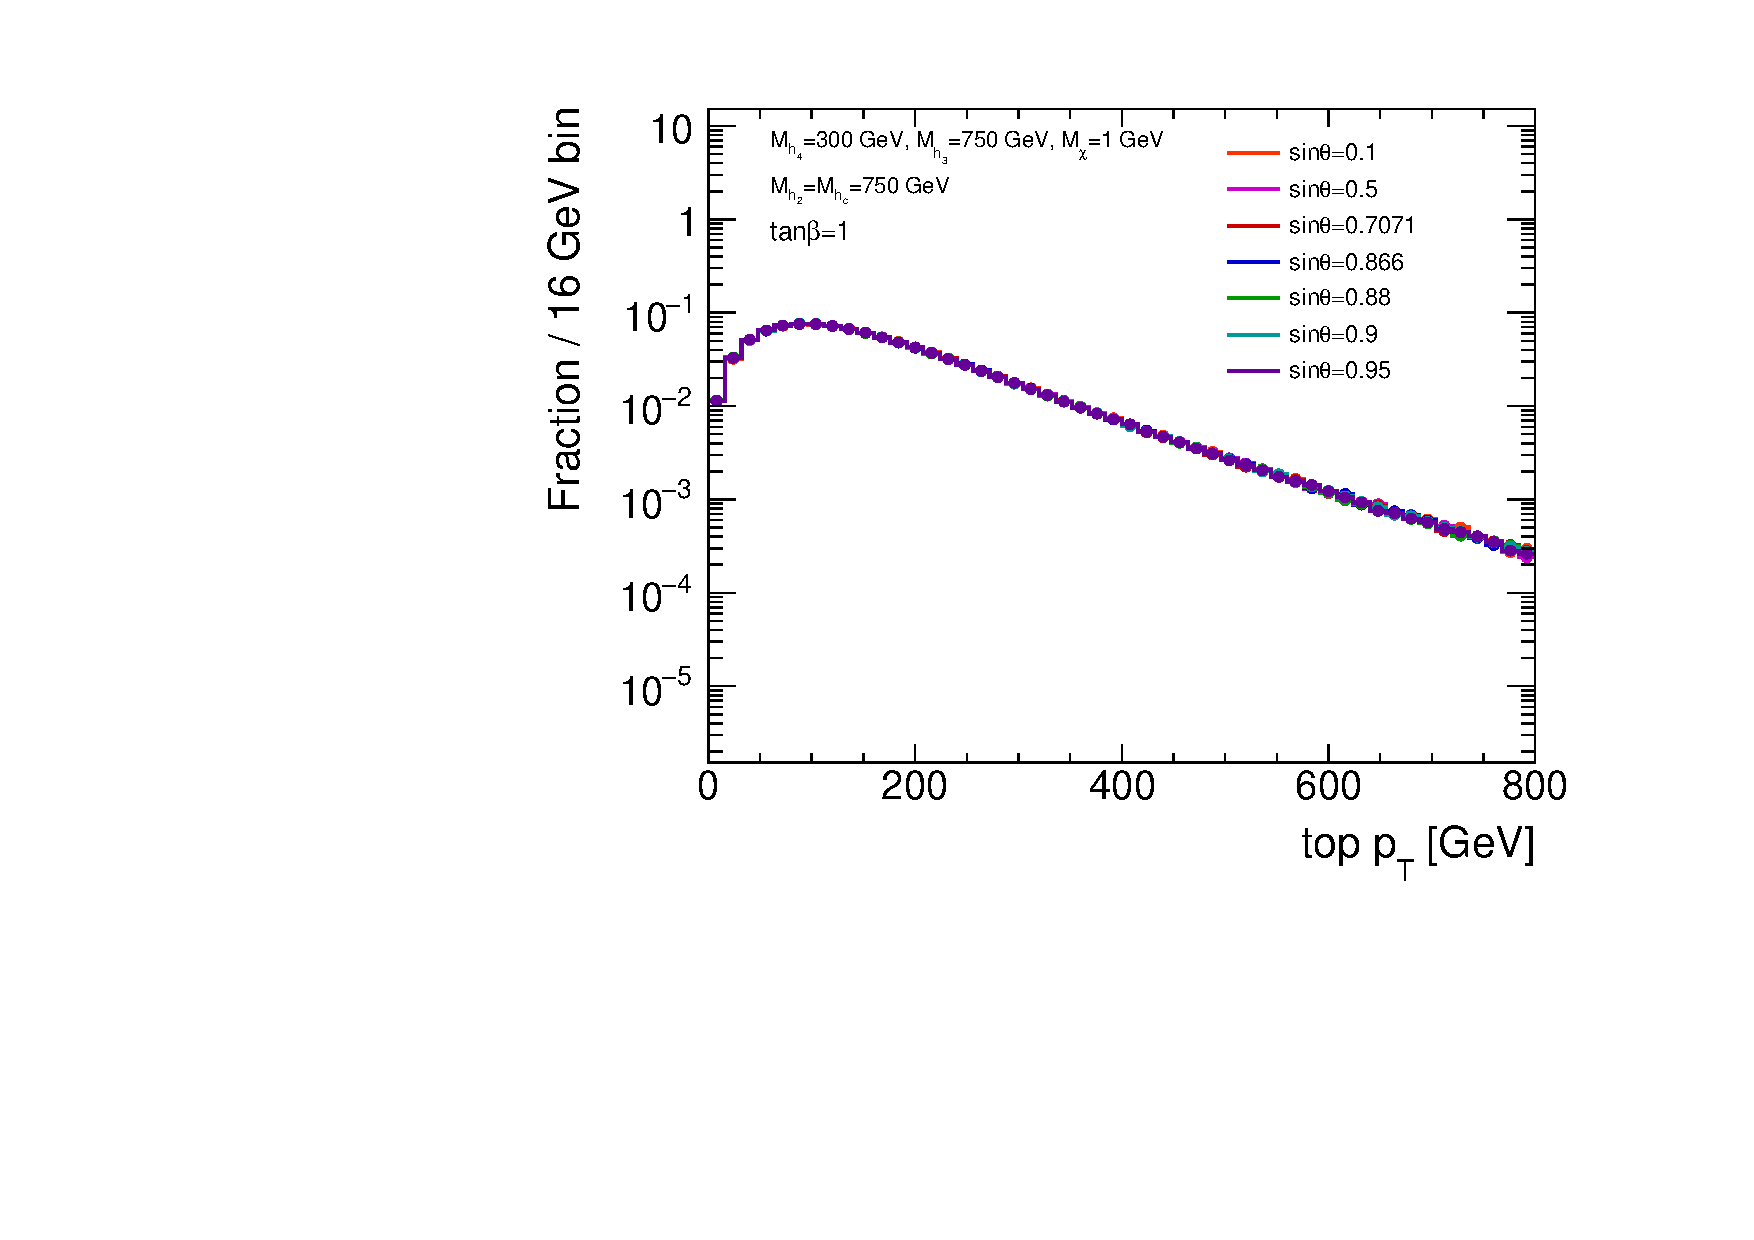
\includegraphics[width=\textwidth]{texinputs/04_grid/figures/DMHF/benchmarking/MDM_1_Ma_300_MA_750_tanb_1.0_SCAN_sinp_v2/topptlog.pdf}
    \caption{top $p_{T}$}
  \end{subfigure}
  \caption{The $E_{T}^{miss}$ and top $p_{T}$ distribution for inclusive $t\bar{t}+\chi\bar{\chi}$ production for various values of $\sin\theta$, with $\mathrm{M_a}=300$ GeV, $\mathrm{M_A}=750$ GeV, $\mathrm{M_H}=\mathrm{M_{H^{\pm}}}=750$ GeV, and $\tan\beta=1$.}
  \label{fig:kin_sinp}
\end{figure}

\begin{figure}%[!htbp]
	\centering

	\begin{subfigure}[t]{0.75\textwidth}
	\centering
	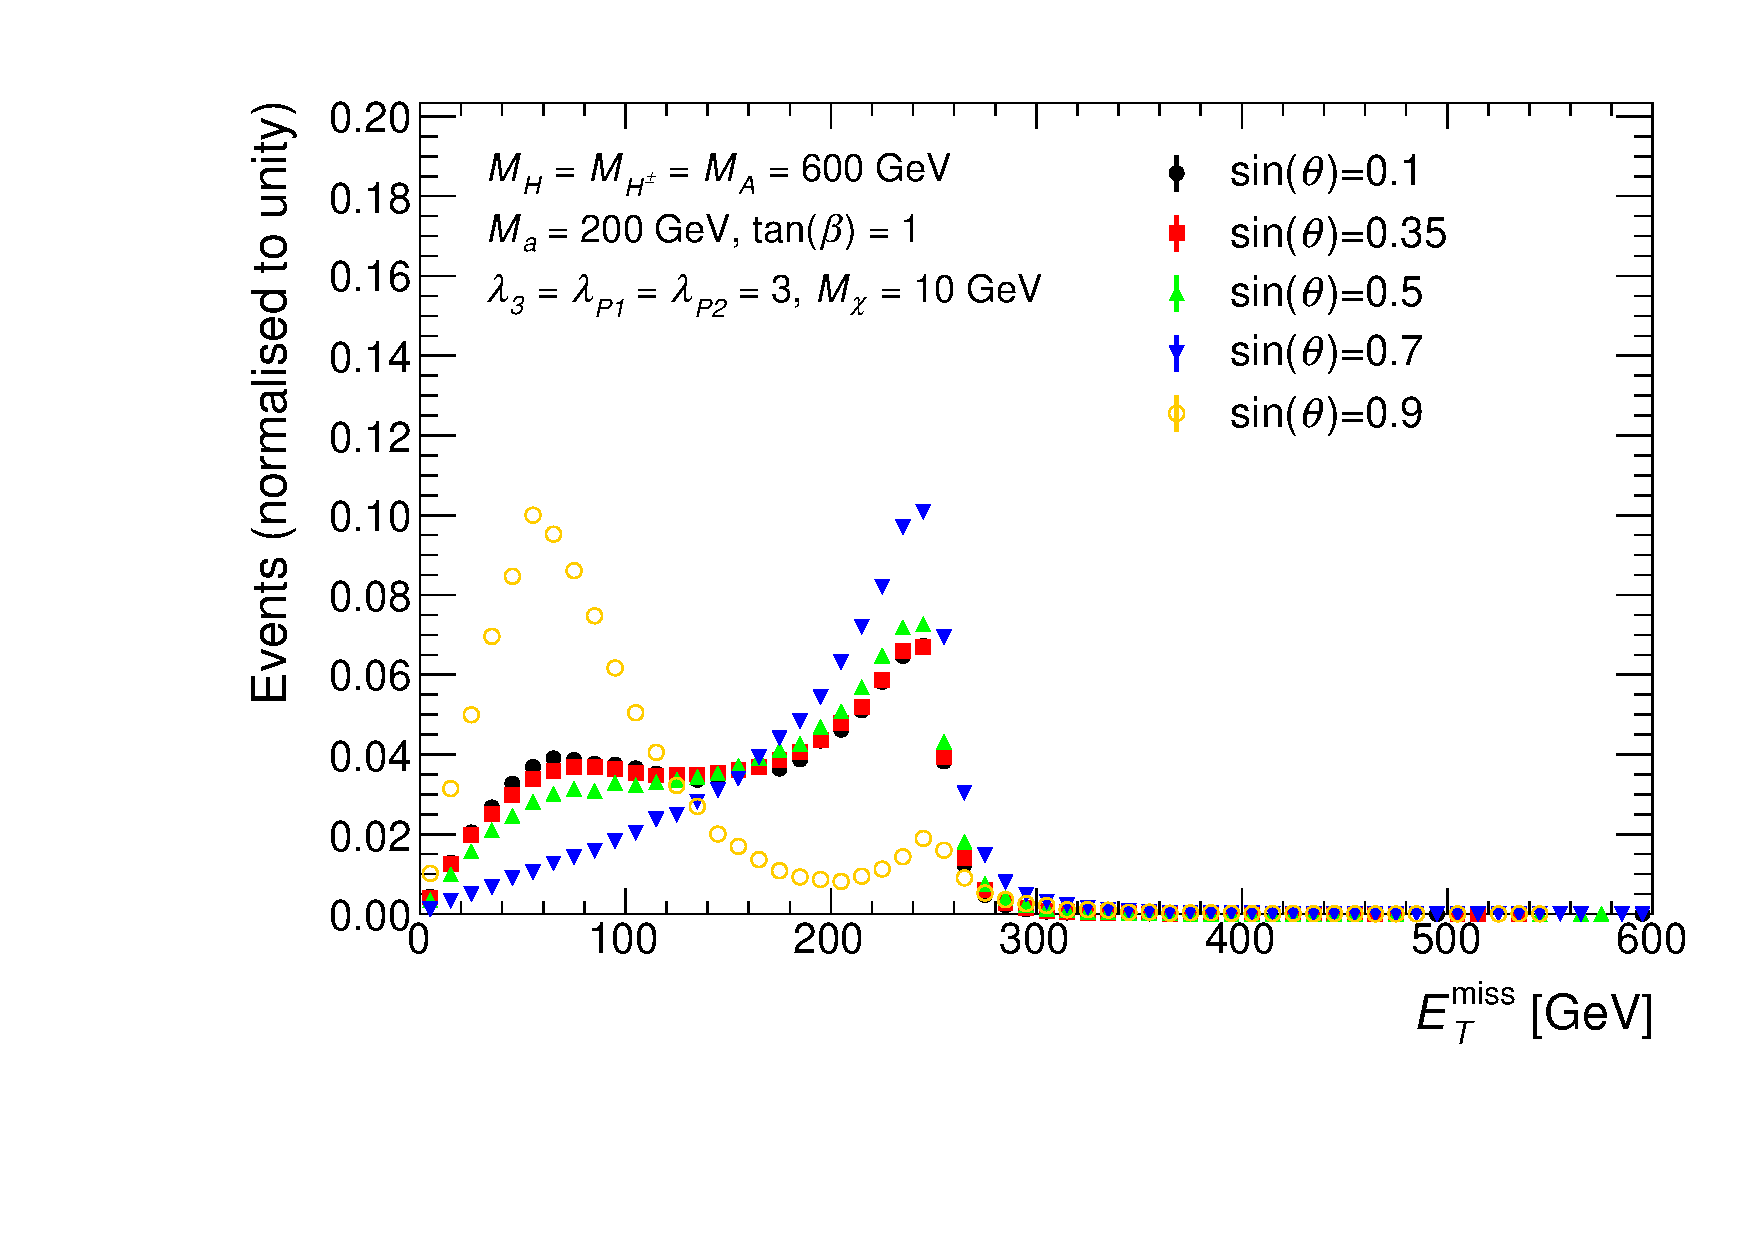
\includegraphics[width=\textwidth]{texinputs/04_grid/figures/monoHbb_sinp_scan_MA600_Ma200_MET_liny_norm2one.pdf}
	\caption{$\MET$ distribution for for five representative models with different $\sinp$ and fixed $\mA = \mH = \mHc = 600 $~GeV, $\ma = 200$~GeV.
	\label{fig:monoHbb_sinp_scan_mA600_ma200_met}} 
    \end{subfigure}
    \begin{subfigure}[t]{0.75\textwidth}
	\centering
	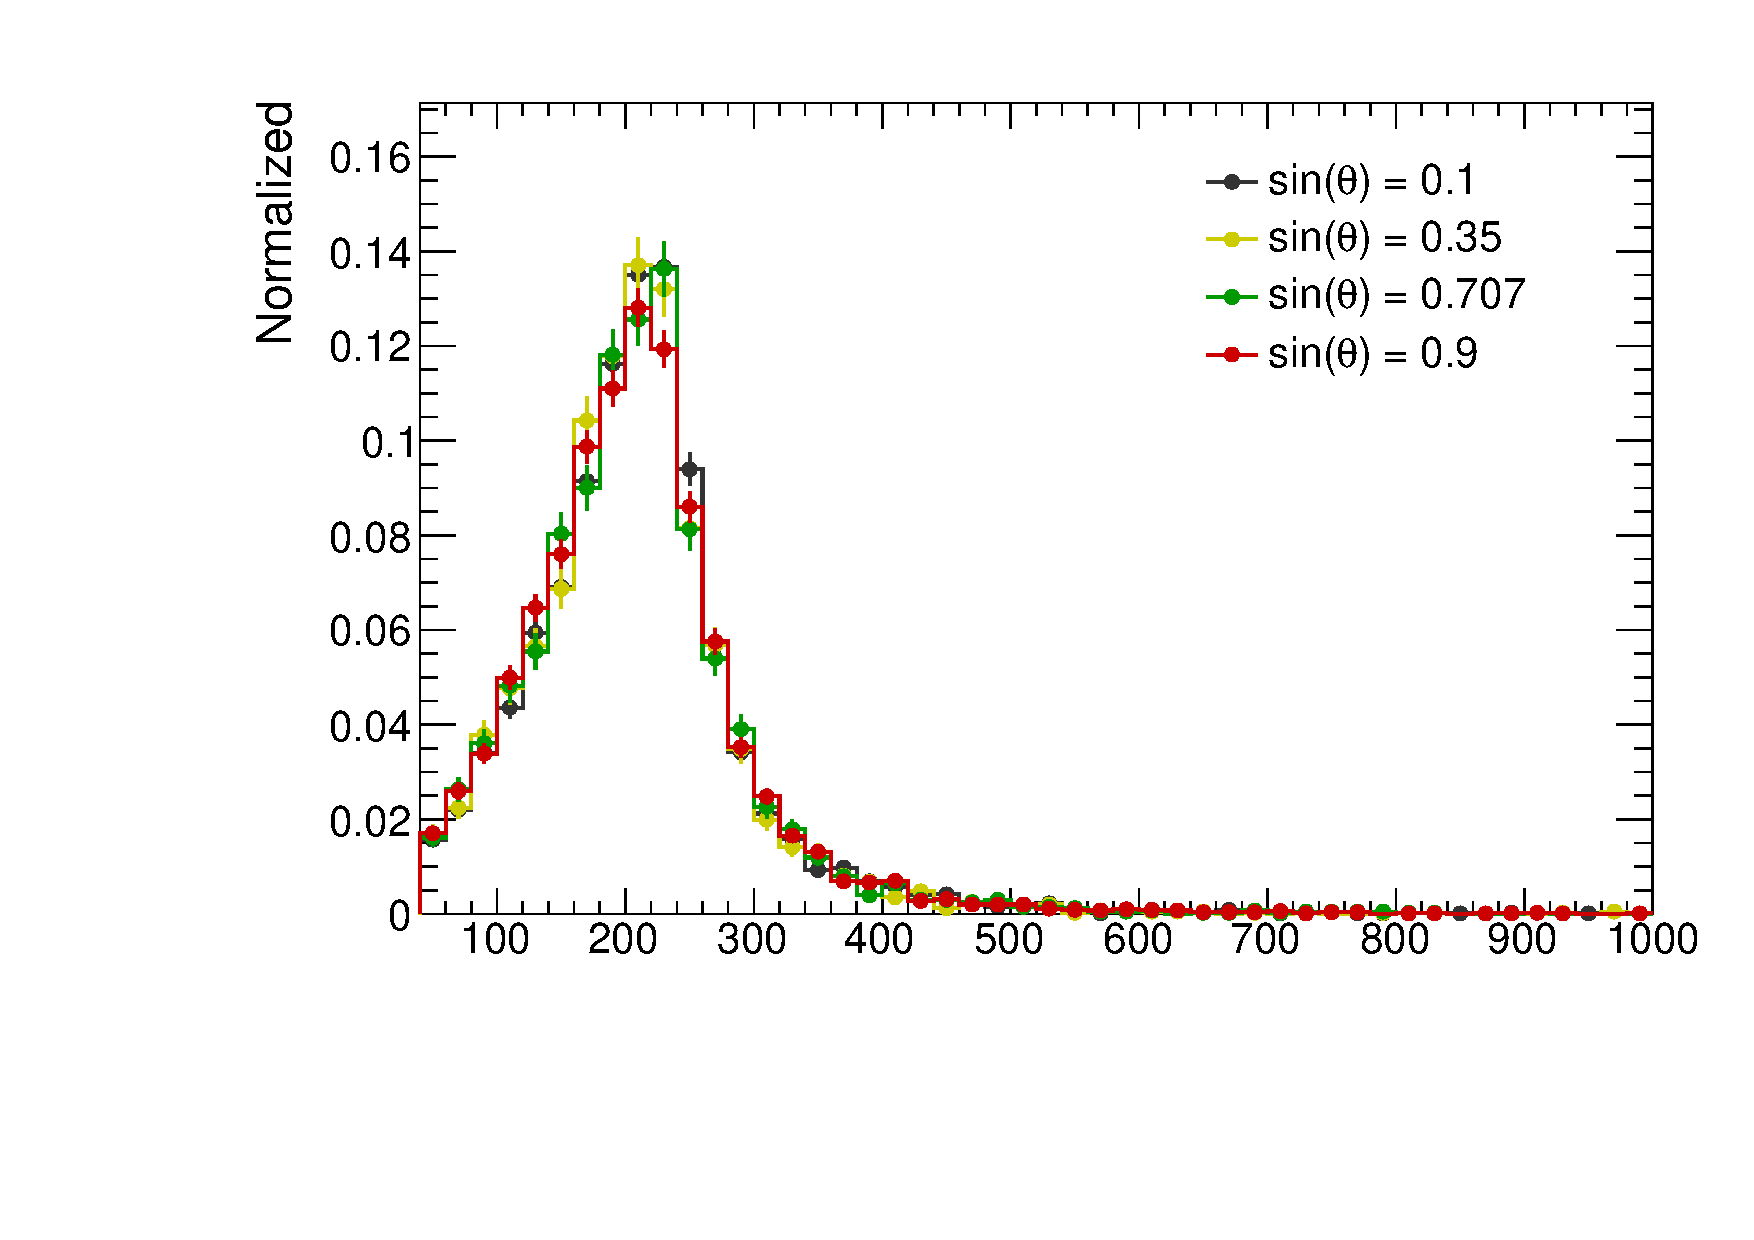
\includegraphics[width=\textwidth]{texinputs/04_grid/figures/monoz/leptonic/SinpScan_mA600_ma250_MET.pdf}	
	\caption{\MET distribution after preselection for scans of $\sin{\theta}$ for fixed $\mA = \mH = \mHc = 600 $~GeV and \ma = 250.
	\label{fig:monoz_kin_sintheta}}
    \end{subfigure}
    
    \caption{$\MET$ distributions in \monohbb and Z(lep)+\MET events for different $\sin{\theta}$. In both cases, $\tanb = 1$ and $\mDM = 10$~GeV. }
    
\end{figure}

In the \monohbb case, the shape of the $\MET$ distribution does not change much  for $\sinp < 0.7$, then changes significantly for $\sinp\geq 0.7$. 
When $\sinp=0.9$, the diagram $gg\rightarrow a\rightarrow A^*h \rightarrow \chi \bar{\chi} h$, producing a \MET peak at around 60~GeV, starts to dominate.
In the Z case, this parameter has little impact on the kinematic distributions.

\begin{figure}
  \centering
  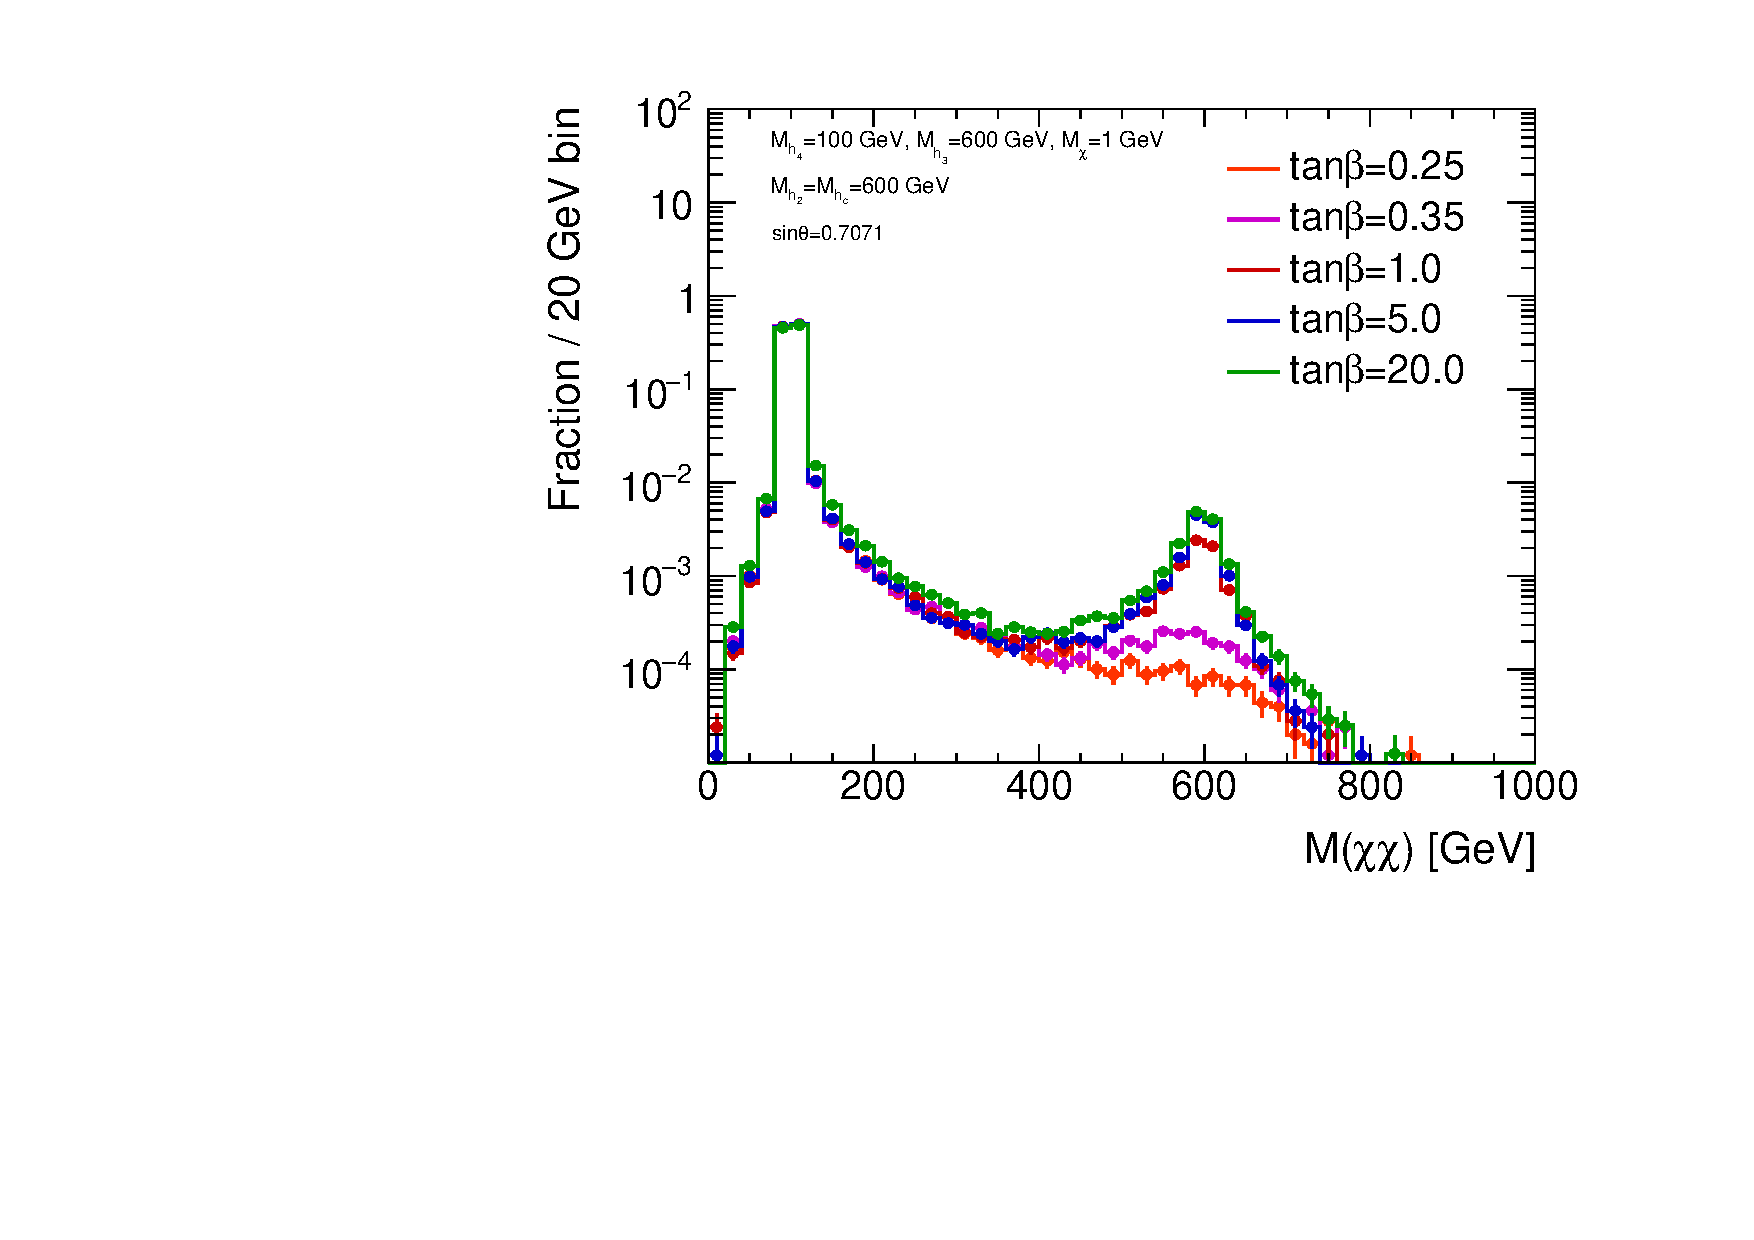
\includegraphics[width=0.6\textwidth]{texinputs/04_grid/figures/DMHF/benchmarking/MDM_1_Ma_100_MA_600_sinp_0.7071_SCAN_tanb_decayed/mchichi.pdf}
  \caption{The mass distribution of the $\chi \bar{\chi}$ system for various values of $\tan\beta$, with $\mathrm{M_a}=100$ GeV, $\mathrm{M_A}=600$ GeV, $\mathrm{M_H}=\mathrm{M_{H^{\pm}}}=600$ GeV, and $\sin\theta=0.7071$.}
  \label{fig:mchichi_tanB}
\end{figure}

\begin{figure}
  \centering
  \begin{subfigure}[b]{0.49\textwidth}
    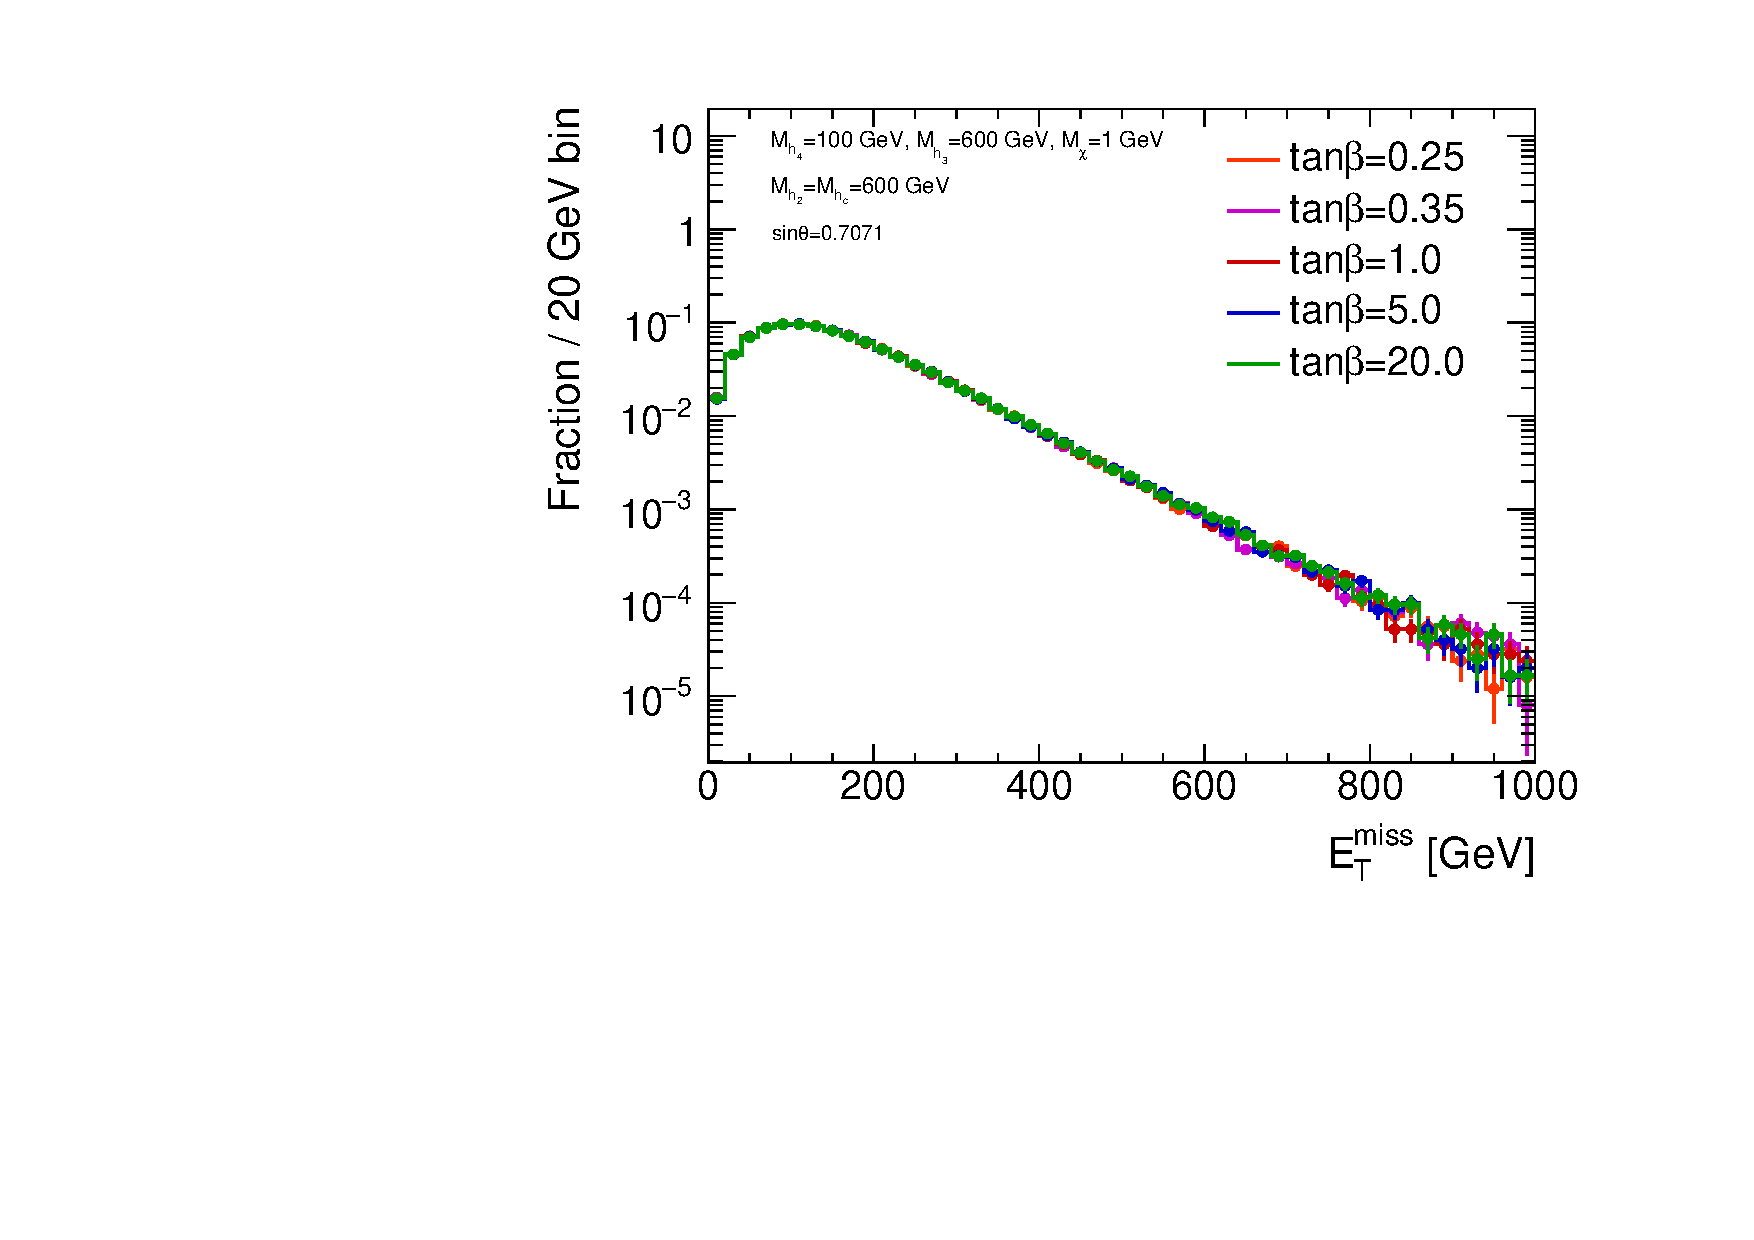
\includegraphics[width=\textwidth]{texinputs/04_grid/figures/DMHF/benchmarking/MDM_1_Ma_100_MA_600_sinp_0.7071_SCAN_tanb_decayed/metlog.pdf}
    \caption{$E_{T}^{miss}$}
  \end{subfigure}
  \begin{subfigure}[b]{0.49\textwidth}
    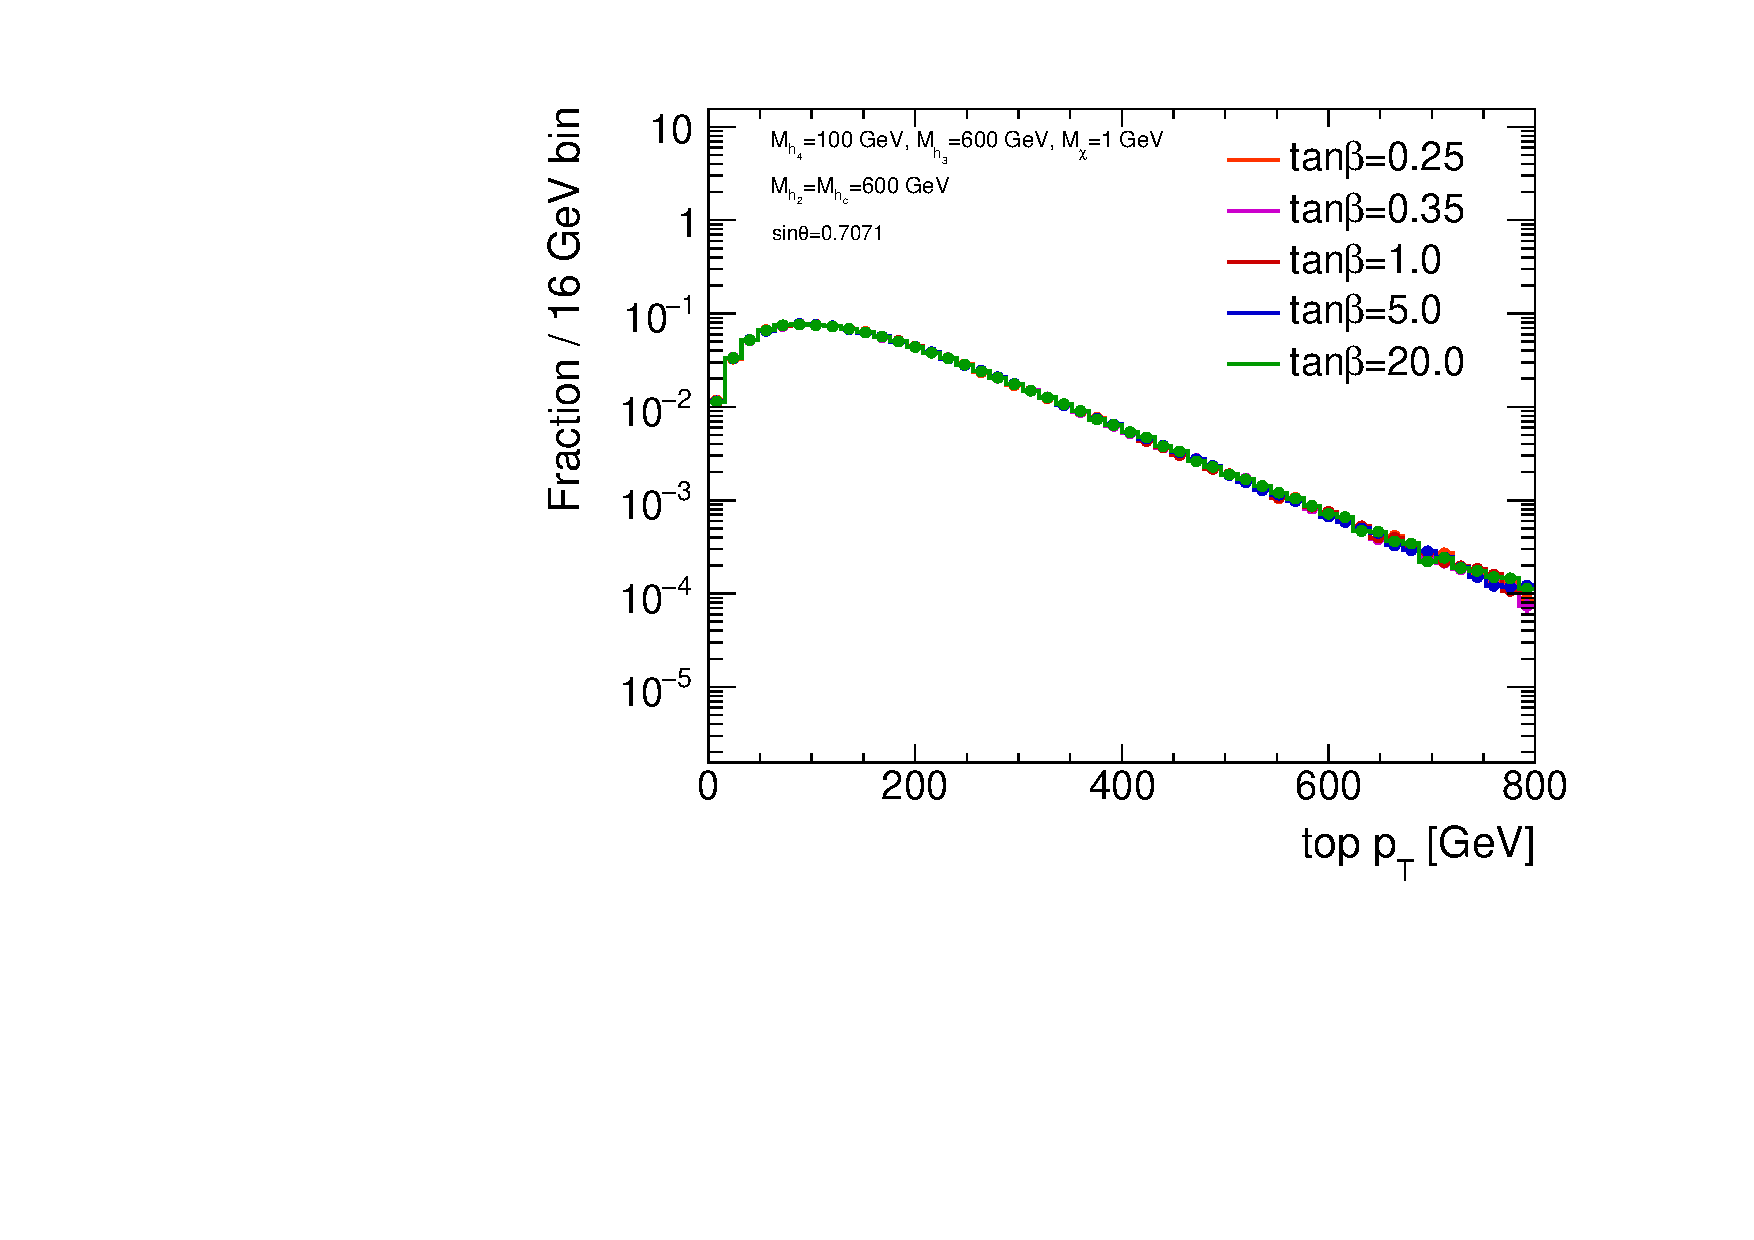
\includegraphics[width=\textwidth]{texinputs/04_grid/figures/DMHF/benchmarking/MDM_1_Ma_100_MA_600_sinp_0.7071_SCAN_tanb_decayed/topptlog.pdf}
    \caption{top $p_{T}$}
  \end{subfigure}
  \caption{The $E_{T}^{miss}$ and top $p_{T}$ distribution for inclusive $t\bar{t}+\chi\bar{\chi}$ production for various values of $\tan\beta$, with $\mathrm{M_a}=100$ GeV, $\mathrm{M_A}=600$ GeV, $\mathrm{M_H}=\mathrm{M_{H^{\pm}}}=6
00$ GeV, and $\sin\theta=0.7071$.}
  \label{fig:kin_tanB}
\end{figure}

%Mixing of the CP-odd weak eigenstates is achieved through the mixing angle, $\theta$. 
The $A$  ($h_{3}$ in the figure) and $a$  ($h_{4}$ in the figure) mass peaks are quite narrow in the $t\bar{t}$ + \MET signature for values where $\sin\theta$ approaches 1, and $a\rightarrow\chi\bar{\chi}$ is the dominant $\chi\bar{\chi}$ production mode, as shown in \autoref{fig:mchichi_sinp}. However, no kinematic dependence on $\sin\theta$ is observed in the $E_{T}^{miss}$ and top quark $p_{T}$ as shown in \autoref{fig:kin_sinp}.

\subsubsection{Ratio of the doublet vacuum expectation values ($\tanb$)}

%%% text related to tanbeta-ma scan
The shape of \MET\ distribution also has a non-trivial dependence on \tanb, as can be seen in \autoref{fig:monoHbb_tanb_scan_met}.
As discussed in the sensitivity study later, at small \tanb, the Yukawa coupling to top quark is large and the signal production mode is dominated by the non-resonant 3-body processes $gg\rightarrow h\chi\bar{\chi}$, which gives a broad and soft \MET\ spectrum. 
As \tanb increases, the contribution of resonant production increases as well and the Jacobian peak also appears.
When the pseudoscalar $A$ is produced off-shell, i.e. when $\mA<\ma+\mh$, the shapes of \MET\ distributions become similar and the dependence on \tanb disappears.

For small values of $\tanb$ there is a slight softening and broadening of the \MET distribution caused by the increased contribution from non-resonant $Z+a$ production in Z+\MET searches. 

\begin{figure}[tbp]
\centering
\begin{subfigure}{0.48\textwidth}
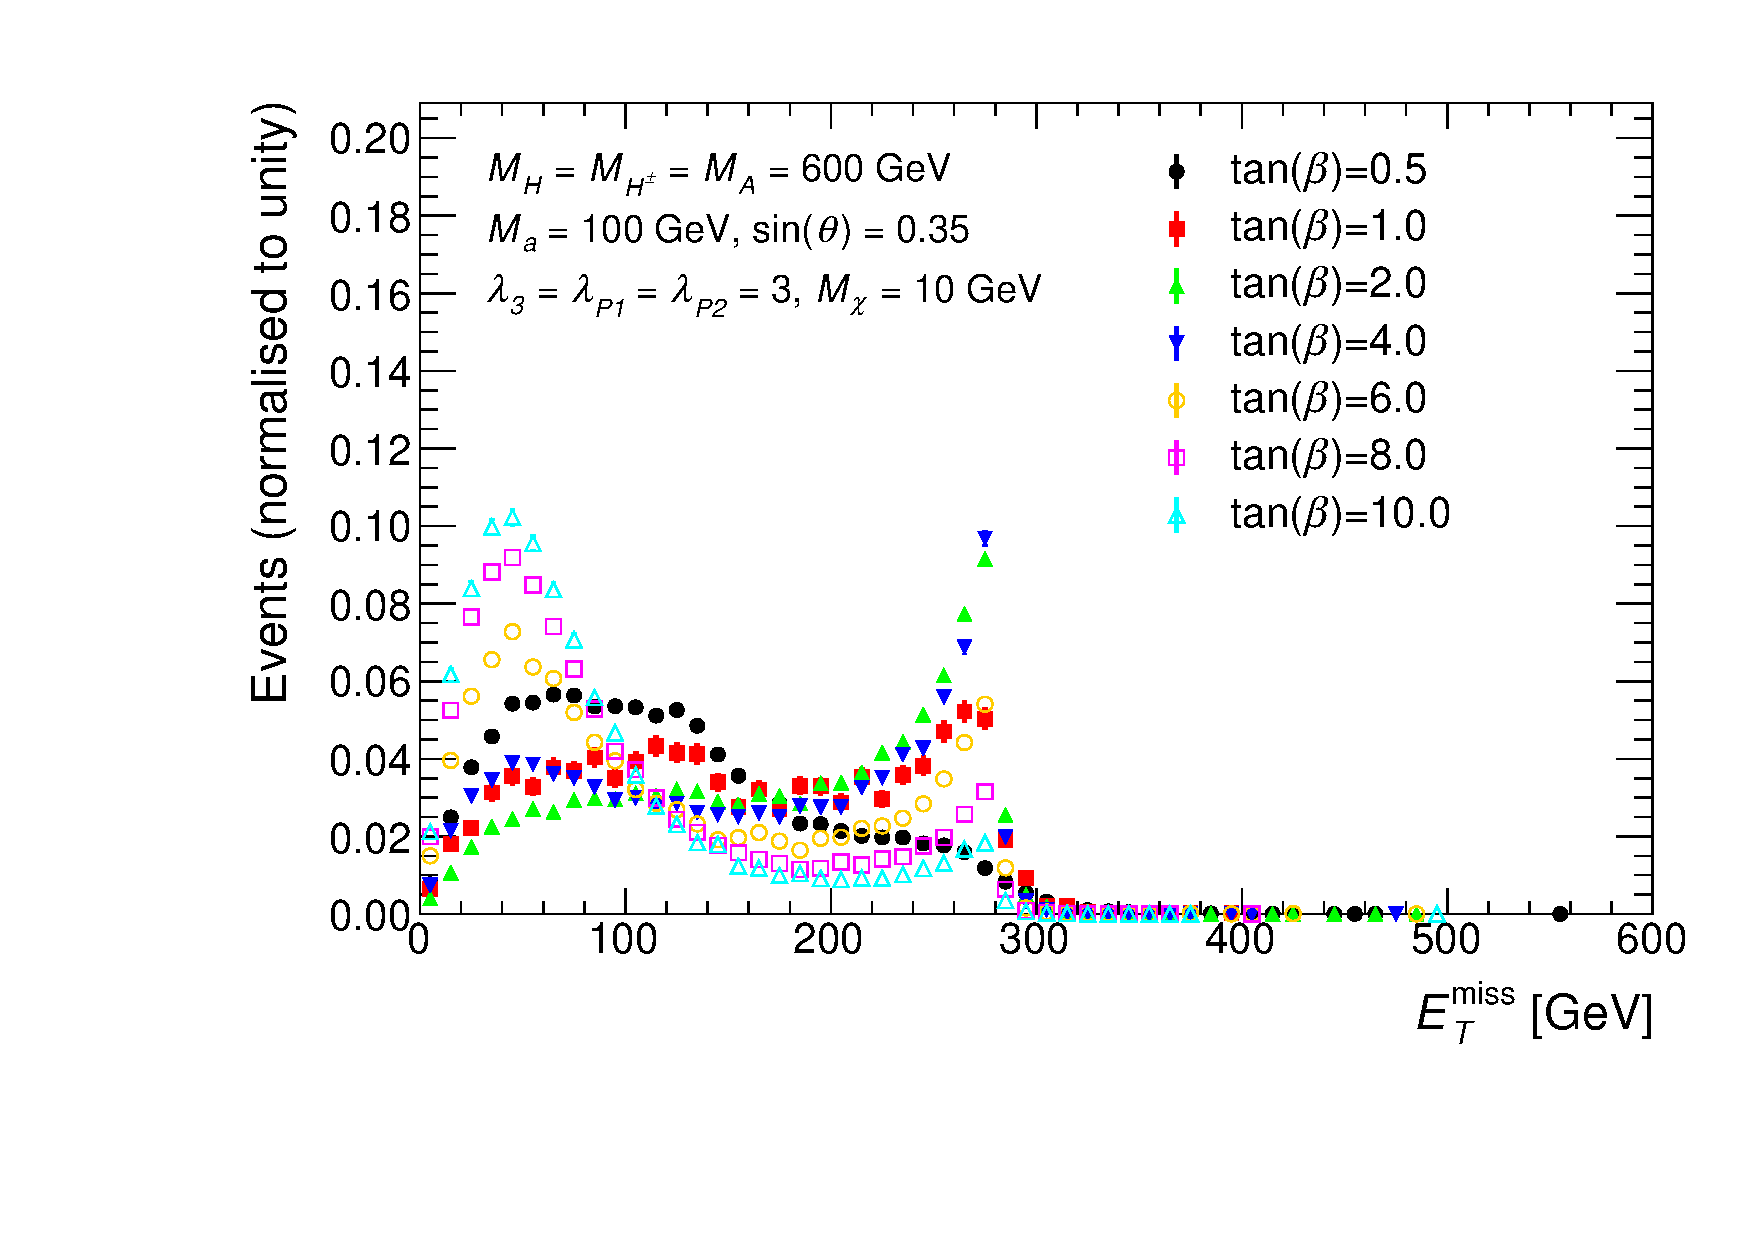
\includegraphics[width = \textwidth]{texinputs/04_grid/figures/monoHbb_tanb_scan_MA600_Ma100_MET_liny_norm2one.pdf}
\end{subfigure}
~
\begin{subfigure}{0.48\textwidth}
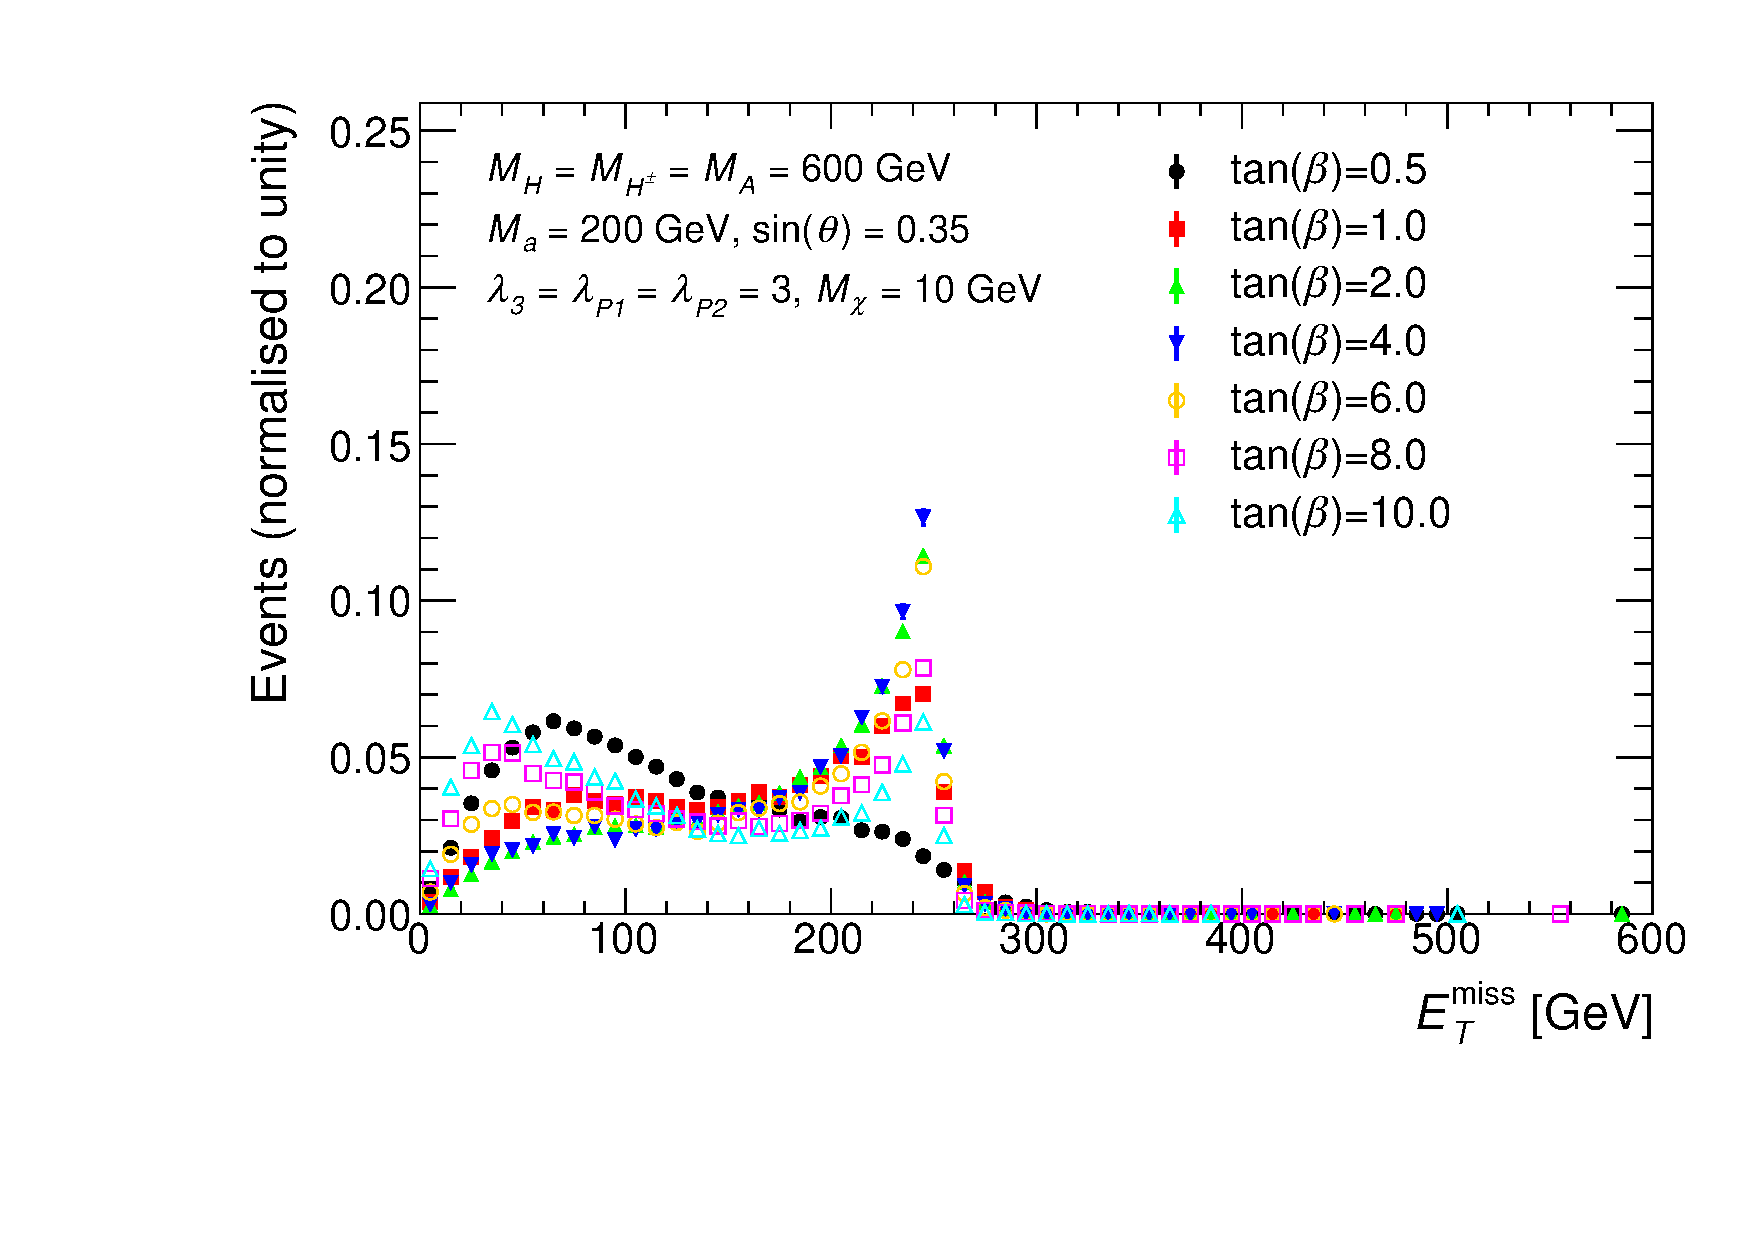
\includegraphics[width = \textwidth]{texinputs/04_grid/figures/monoHbb_tanb_scan_MA600_Ma200_MET_liny_norm2one.pdf}
\end{subfigure}
\\
\centering
\begin{subfigure}{0.48\textwidth}
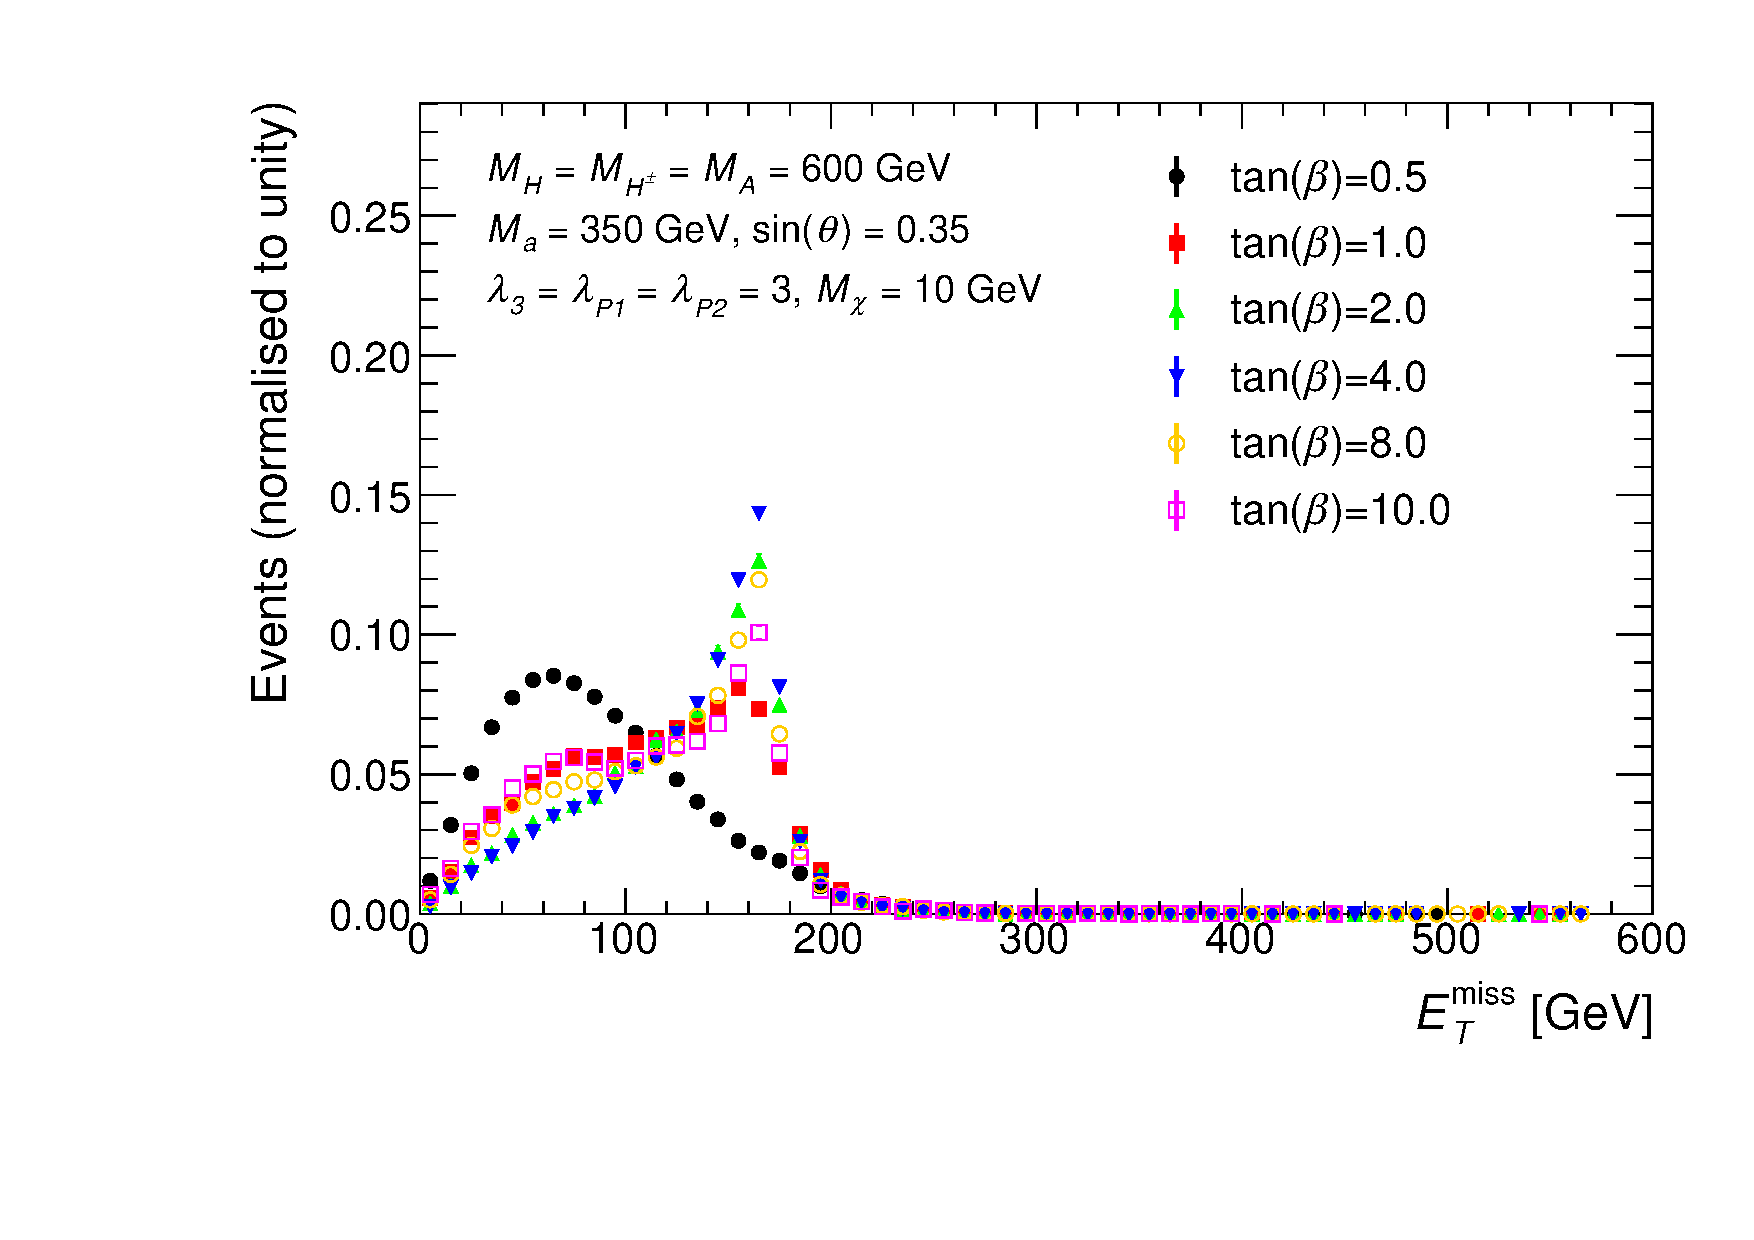
\includegraphics[width = \textwidth]{texinputs/04_grid/figures/monoHbb_tanb_scan_MA600_Ma350_MET_liny_norm2one.pdf}
\end{subfigure}
~
\begin{subfigure}{0.48\textwidth}
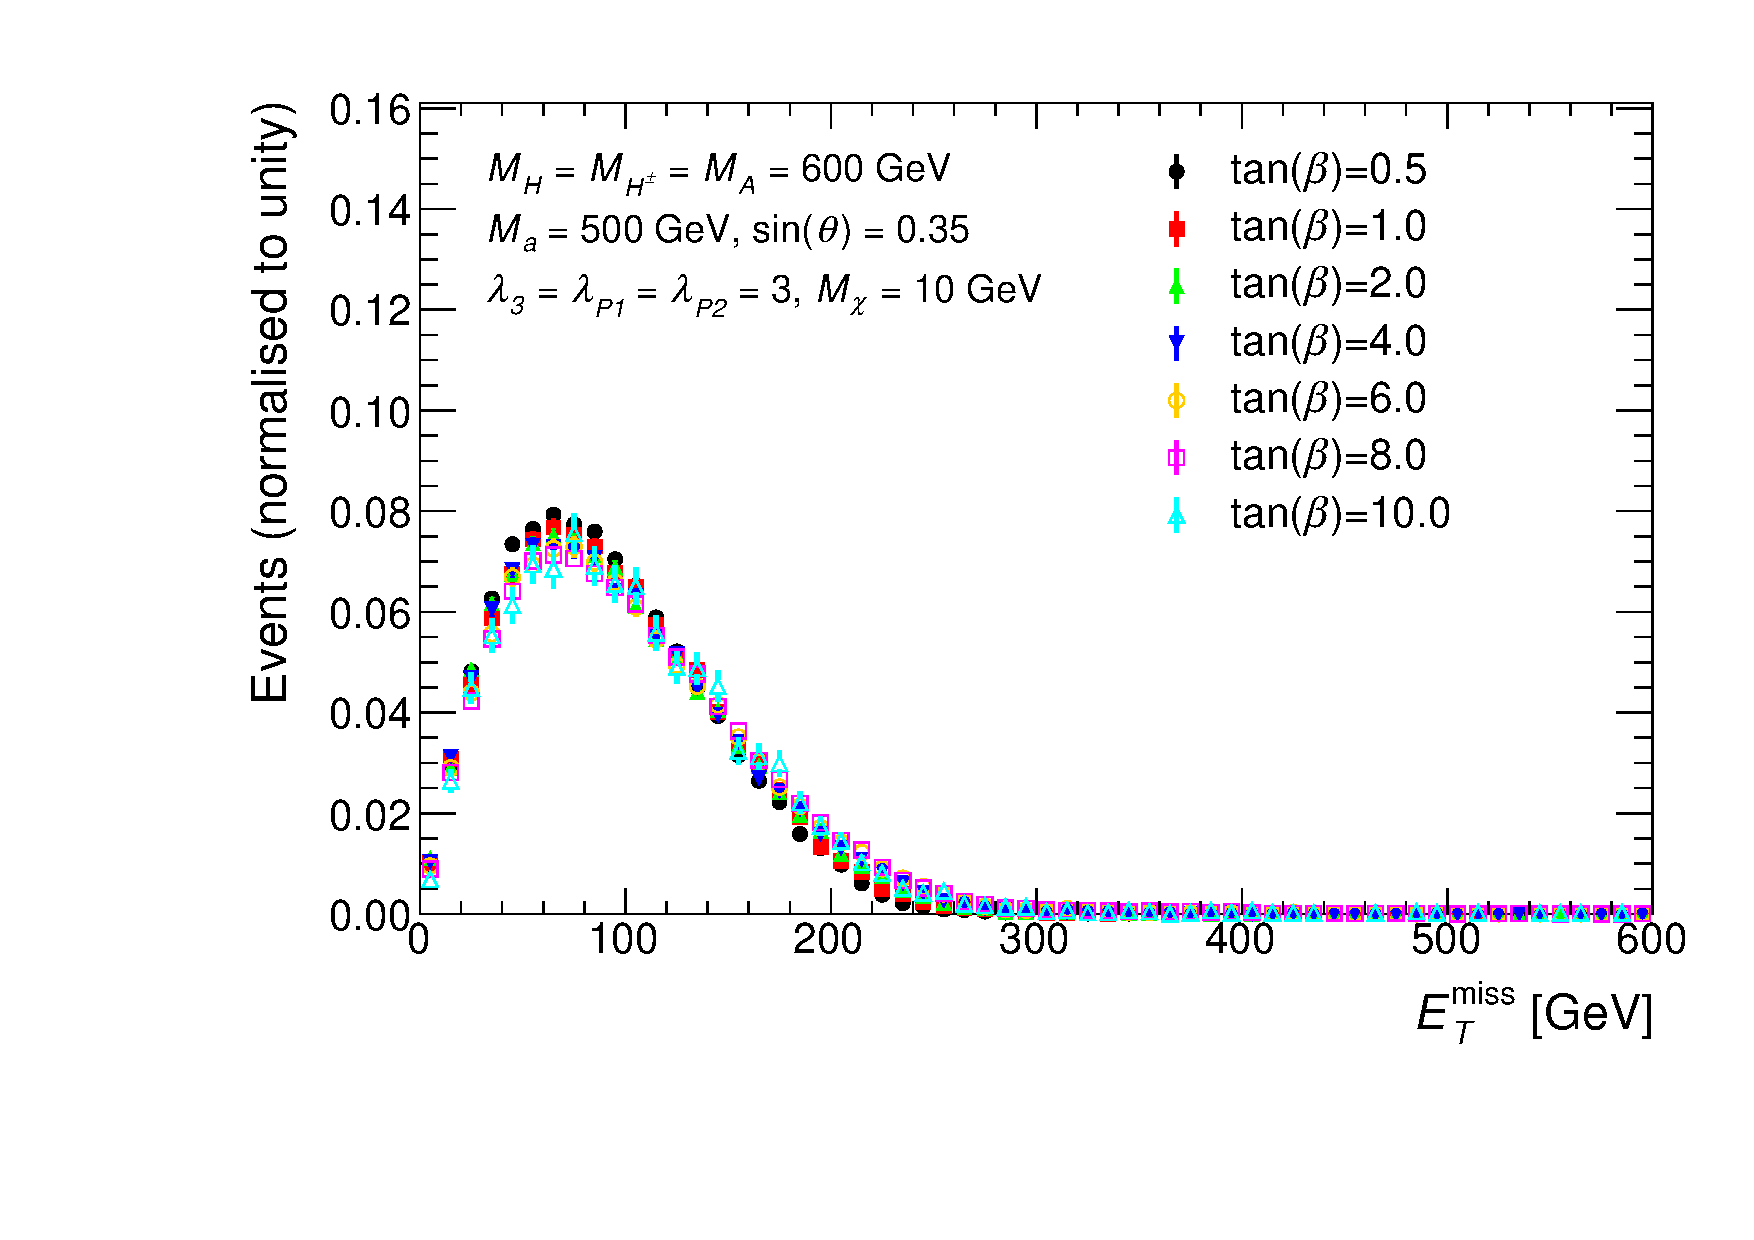
\includegraphics[width = \textwidth]{texinputs/04_grid/figures/monoHbb_tanb_scan_MA600_Ma500_MET_liny_norm2one.pdf}
\end{subfigure}
\caption[$\MET$ distribution in $h\rightarrow bb + \MET$ events for different 
$\tanb$ for $\mA = \mH = \mHc = 600 $ GeV]
{
Missing transverse momentum distribution of $h\rightarrow bb + \MET$ signal 
events at parton level with different $\tanb$ and
 fixed $\mA = \mH = \mHc = 600 $~GeV, $ \mDM = 10$~GeV, $\sinp = 0.35$, 
and $ \lap1 = \lap2 = \lam3 = 3 $. The values of $\ma$ are set to 100, 200, 
350, and 500~GeV, respectively.
The shapes of the $\MET$ distributions for different $\tanb$ are similar when 
$\mA < \mh+\ma$. Note, in these figures, both the contributions of $gg$ and $b\bar{b}$ 
initiated processes are included and a combined histogram is produced 
according to their corresponding cross sections.
}
\label{fig:monoHbb_tanb_scan_met}
\end{figure}

\begin{figure}
\centering
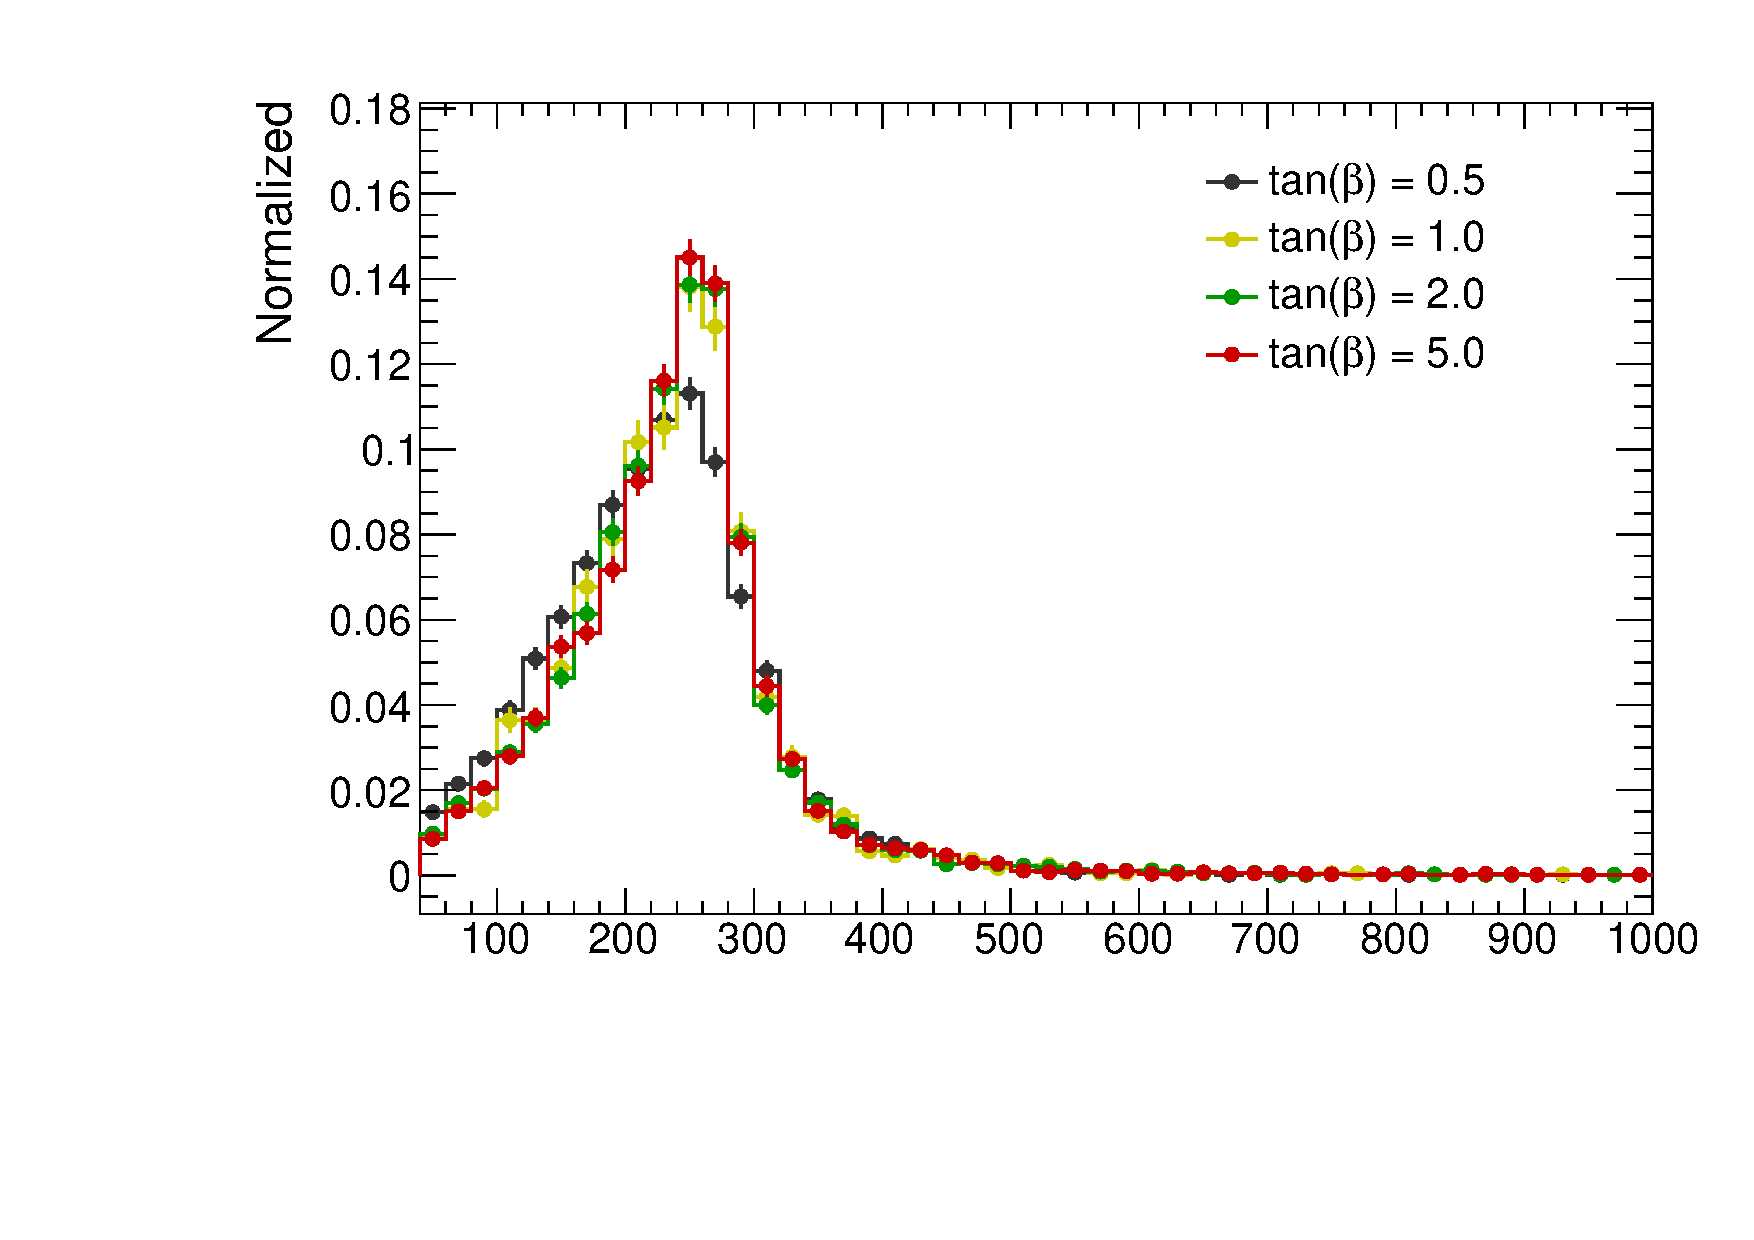
\includegraphics[width=0.48\textwidth]{texinputs/04_grid/figures/monoz/leptonic/TanbScan_mA600_ma150_MET.pdf} 
\caption{\MET distribution after preselection for scans of $\tan{\beta}$ for fixed \mA =600 \GeV and \ma = 150 \GeV. This parameter has little impact on the kinematic distributions, except for small values of \tanb where there is a slight softening and broadening of the \MET distribution caused by the increased contribution from the top box feynman diagram.}
\label{fig:monoz_kin_tanb}
\end{figure}


In the $t\bar{t}$ + \MET signature, and in the limit of small $\tan\beta$ values, the couplings of $A$ ($h_{3}$ in the figure) and $a$ ($h_{4}$ in the figure) to down-type quarks are heavily suppressed regardless of the Yukawa assignment. At LO, $t\bar{t}+\chi\bar{\chi}$ associated production is mediated through either CP-odd weak eigenstate, $A$ or $a$, though it is shown in Fig.~\ref{fig:mchichi_tanB} that $a\rightarrow\chi\bar{\chi}$ is the dominant production mode. Although the relative mediator contribution is dependent on $\tan\beta$, observables such as $E_{T}^{miss}$ and top quark $p_{T}$ do not have a kinematic dependence on $\tan\beta$ as demonstrated in Fig.~\ref{fig:kin_tanB}. This is because [reasons]. 


\subsubsection{Mass of DM fermion ($\mDM$)}

The mass of the DM fermion $\mDM$ can change the total cross section and shape of the $\MET$ distribution, depending on the mass hierarchy of the $A,a,h,\chi$ particles. This is demonstrated in \autoref{fig:monoHbb_mDM_scan_met}. 
Provided on-shell  decays $a\to\chi\chi$ are possible, i.e., $\mDM < \ma/2$, the exact value of \mDM has no effect on either kinematics or the total cross section. 
The only exception is the case $\ma/2 > \mDM > \frac{1}{2}(\ma - M_h)$. In this  $\mDM$ range, the non-resonant process $a \to h A^*\left(\chi\chi\right) $ is kinematically inaccessible. 
This reduces the overall cross section relative to the $\mDM \leq \frac{1}{2}(\ma - M_h)$ case, and slightly changes the soft part of the total $\MET$ spectrum. 
However, since the contribution of the $a \to h A^*\left(\chi \chi\right)$ process is minor in any case, the differences are negligible.

If the DM particle mass is exactly on threshold, i.e., $\mDM = \ma/2$, the total cross section is resonantly enhanced. 
This resonant threshold enhancement drops rapidly towards both higher and lower $\mDM$. Furthermore, the shape of the $\MET$ distribution at threshold, where amplitudes involving $a\to\chi\chi$ decays make up a larger fraction of the signal, differs significantly from the one below threshold. 
Below threshold ($\mDM > \ma/2$), the total cross section quickly drops by several orders of magnitude. In this regime, the shape of the $\MET$ distribution changes with $\mDM$ continuously.

\begin{figure}[tbp]
\centering
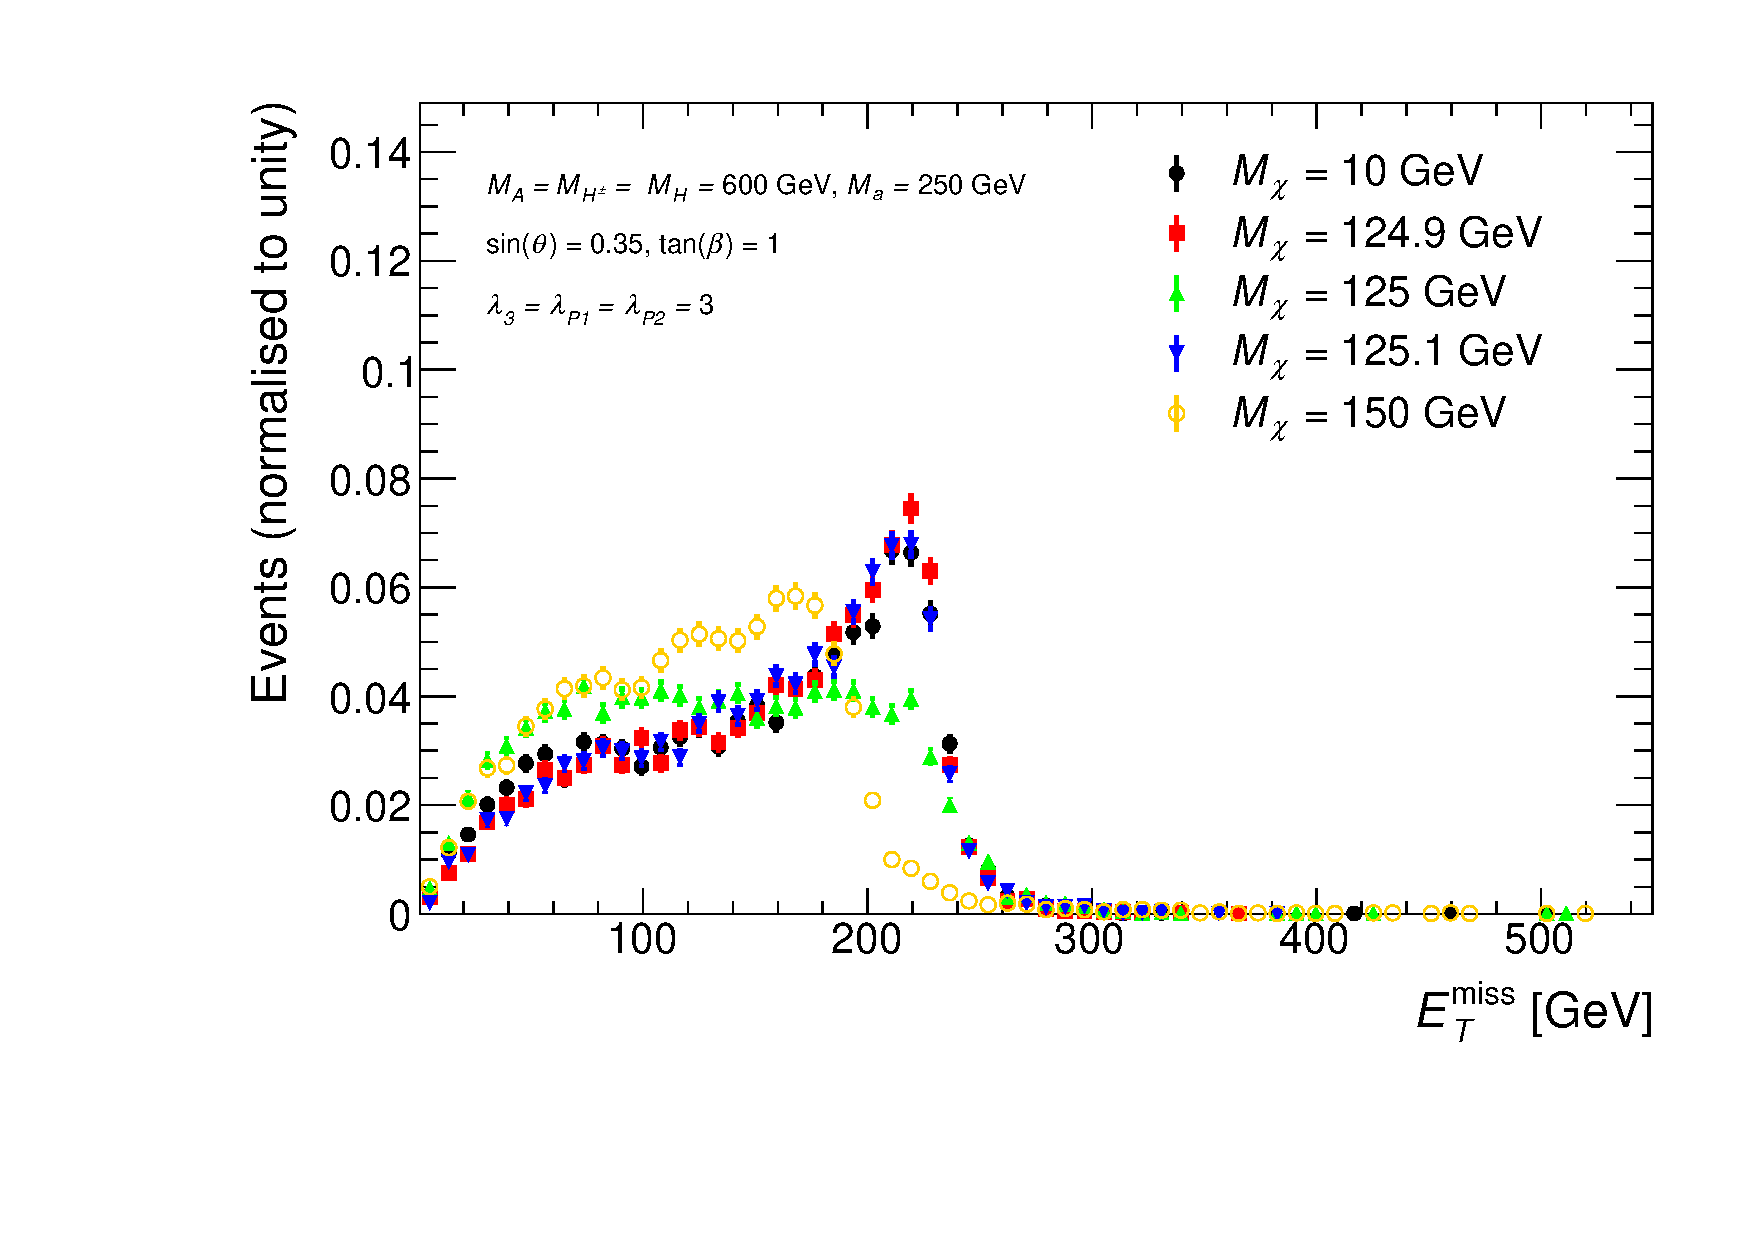
\includegraphics[width=0.7\textwidth]{texinputs/04_grid/figures/monoHbb_mDM_scan_MET_liny_norm2one.pdf}
\caption[$\MET$ distribution in \monohbb events for different $\mDM$]
{
Missing transverse momentum distribution  of \monohbb signal events at parton level for five representative models with different $\mDM$
and fixed $\mA = \mH = \mHc = 600 $ GeV $\ma = 250$ GeV, $ \sinp = 0.35, \tanb = 1$ and $ \lap1 = \lap2 = \lam3 = 3 $. 
The shape of the $\MET$ distribution does not change for $\mDM < \ma/2$, then changes significantly for $\mDM>=\ma/2$.
%
}
\label{fig:monoHbb_mDM_scan_met}
\end{figure}

Similar effects are seen in \autoref{fig:dm_scan_ll}. In the $\mDM < \frac{\ma}{2}$ region, \mDM has no effect on event yield or \MET distribution, at $\mDM = \frac{\ma}{2}$ a resonant enhancement to the cross section occurs, and in the off-shell region where  $\mDM > \frac{\ma}{2}$ cross section steeply drops.  The \MET shape remains the same up to, and even slightly above, $\mDM = \frac{\ma}{2}$, but further off shell the \MET distribution becomes increasingly disperse.  For \mDM = 200 \GeV, DM can still decay on-shell through the $A$.  For \mDM = 500 \GeV both pseudoscalars are off-shell leading to an event yield too low to fit on the figure on the left and a \MET distribution without structure.

\begin{figure}
\centering
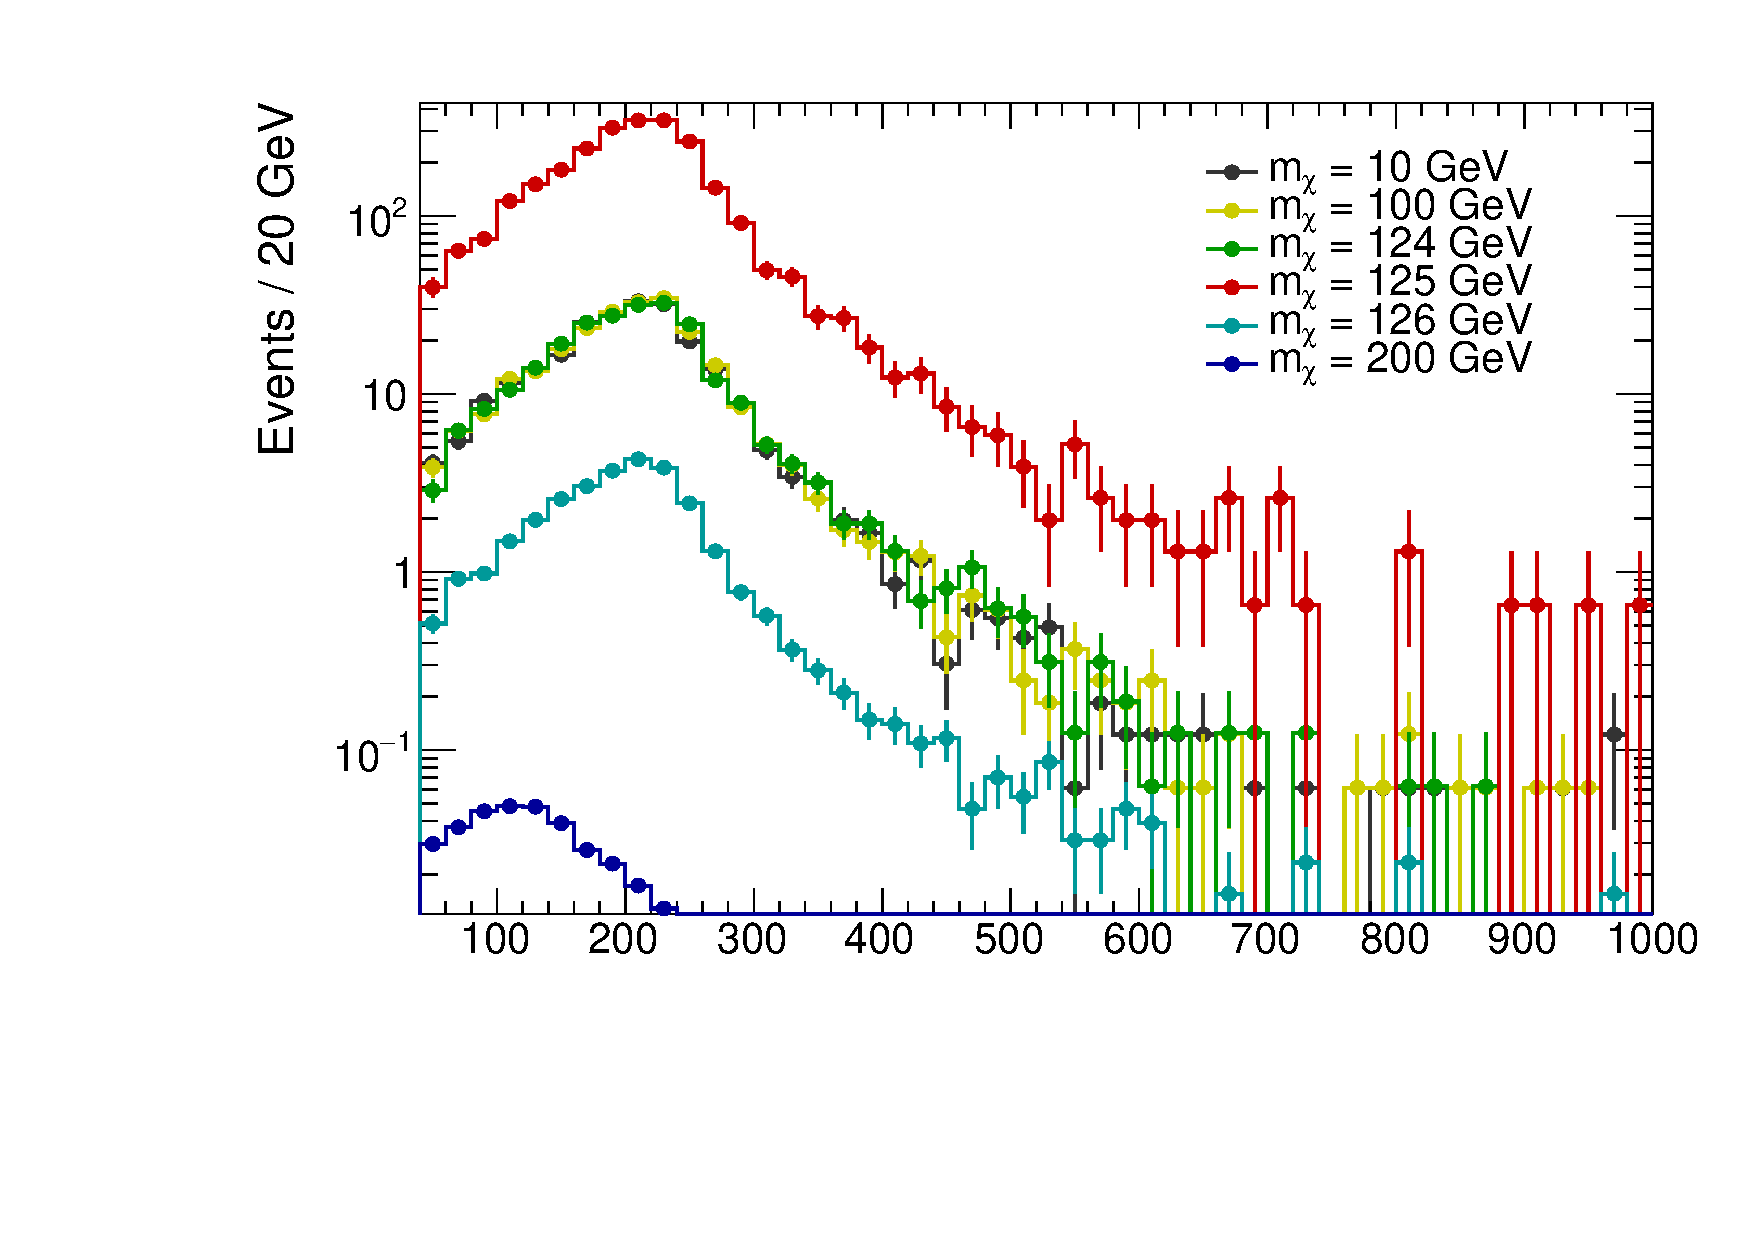
\includegraphics[width=0.48\textwidth]{texinputs/04_grid/figures/monoz/leptonic/mDMScan_mA600_ma250_MET.pdf}
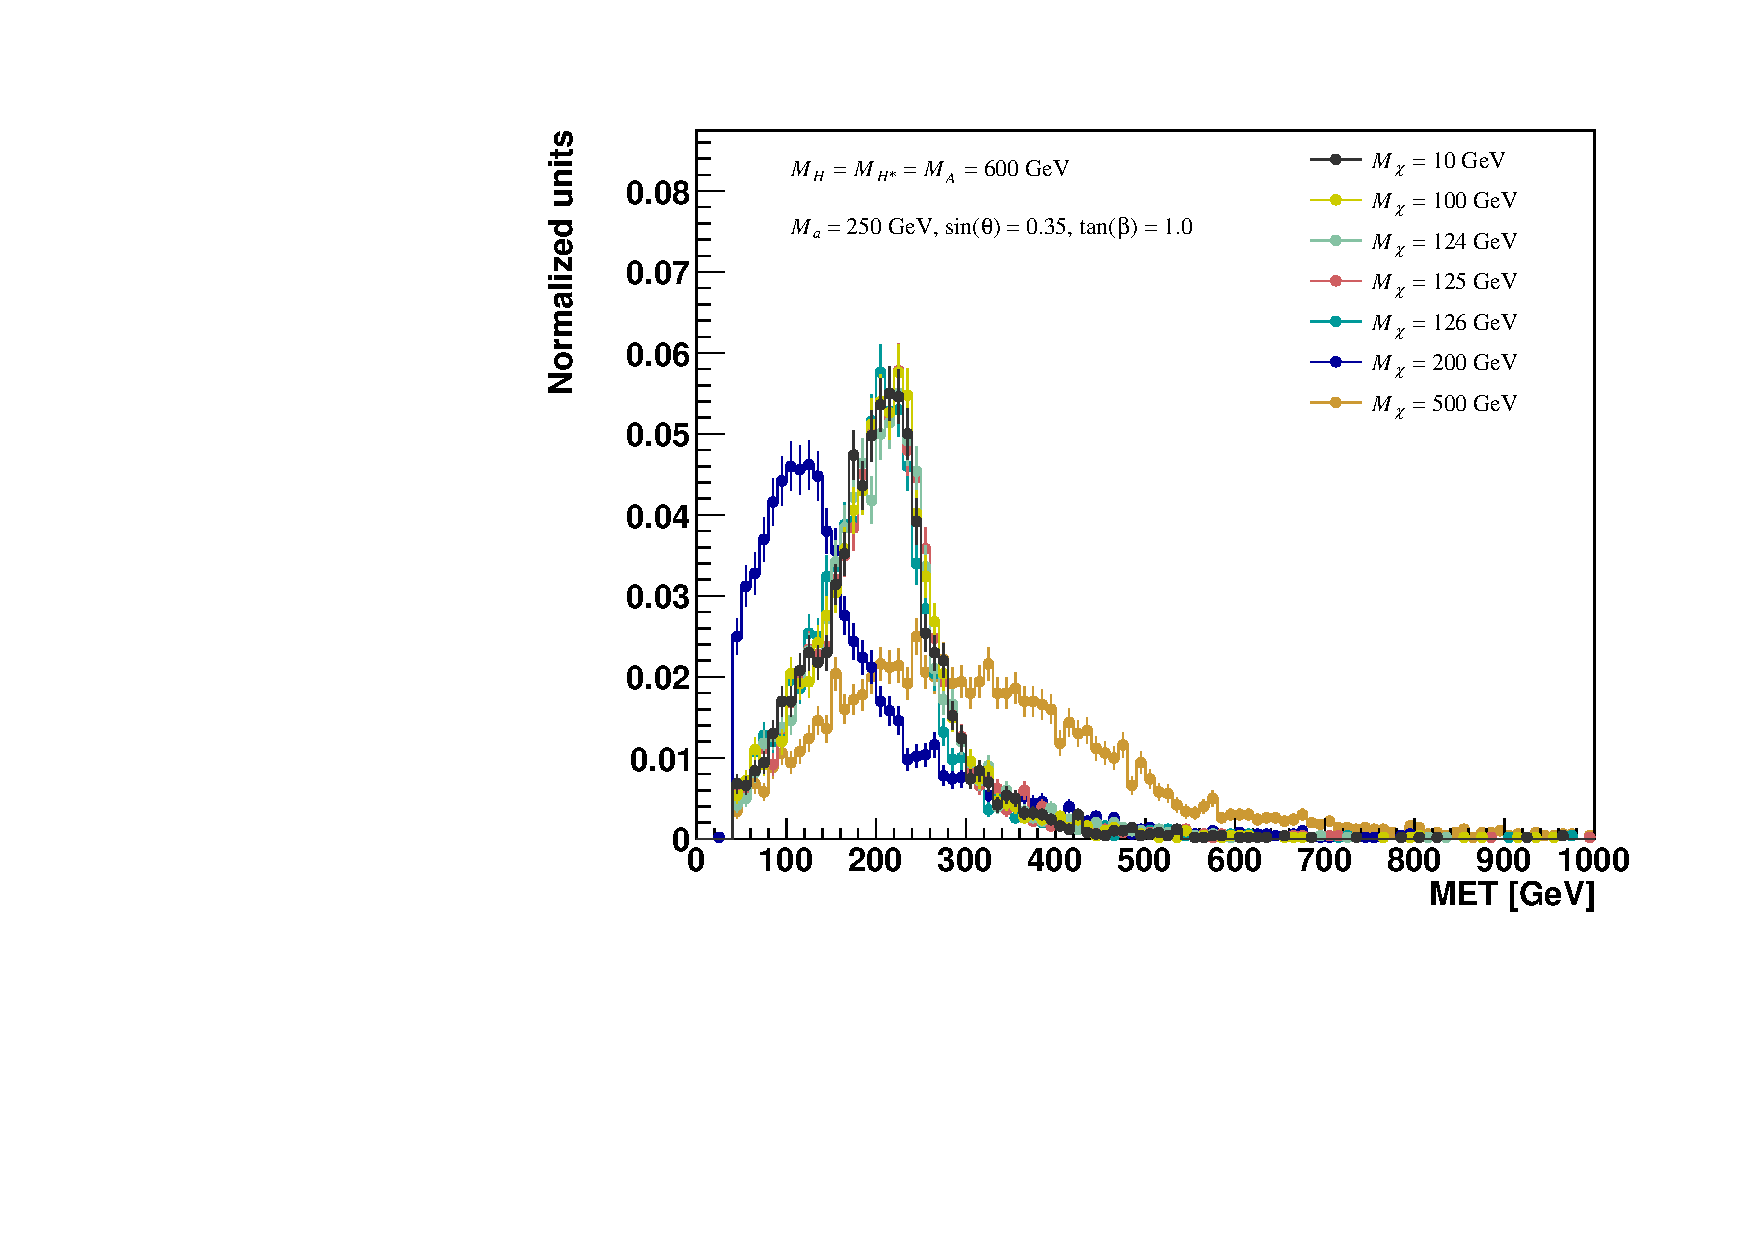
\includegraphics[width=0.47\textwidth]{texinputs/04_grid/figures/monoz/leptonic/mDMscan_ma250.pdf}
\caption{\MET distributions following preselection in the Z(lep) +\MET search are shown (left) scaled to 40 \ifb and (right) normalized to unity for different values of \mDM with fixed \mA = 600 \GeV and \ma = 250 \GeV.}
\label{fig:dm_scan_ll}
\end{figure}

A value of $\mDM$=10 is chosen for the following studies, as it produces a cross-section that is sufficiently large for this model to be detected with Run-2 LHC data and highlights the resonant features of the \MET spectrum.
%TODO: mention instability


\section{Parameter grid}

%\paragraph{Logic of how we proceeded}
%
%\begin{itemize}
%\item Starting from benchmark 3 of \cite{Bauer:2017ota}
%\item Mapping the kinematics and sensitivity of the model by scanning some of the
%various parameters
%\item Checking whether other existing models can be rescaled
%\end{itemize}
%
%\subsubsection{Results of studies}
%
%Each of the signatures should have the following plots in the planes
%of the final recommendation: 
%\begin{itemize} 
%\item efficiency at parton level with simplified, published cuts
%\item total and fiducial cross-section at parton level 
%\item 2 - 3 kinematic plots of what has been scanned that are most representative for the analysis (here the analysers decide, then we harmonize at the end)
%\end{itemize} 
%
%Signatures:
%
%\begin{itemize}
%
%\item{Mono-Z (lep/had)}
%
%\item{MonoH$\rightarrow$bb}
%
%\item{Monojet}
%
%\item{ttbar+MET}, with specific discussion about rescaling
%
%\item{other signatures who have not yet presented at public meetings, in ATLAS and CMS}
%
%\end{itemize}

%\subsection{Parameter scan}

The studies in the previous section show that varying most of the model parameters lead to non-trivial modifications of the for the H+\MET and Z+\MET searches. 
We decide to investigate the model parameter space through two-dimensional and one-dimensional scans of five parameters: the light pseudoscalar mass (\ma), the heavy pseudoscalar mass (\mA) that we set equal to the mass of the heavy and charged Higgs bosons (\mA = \mH = \mHc), the mixing angle $\sinp$, the ratio of VEVs of the Higgs doublets $\tanb$ and the dark matter particle mass \mDM. 
The benchmark model points that have been agreed within the DMWG and are suggested here do not provide an exhaustive scan the entire parameter space of this model, but highlights many of the features that are unique of this model and showcases the complementarity of the various signatures. 

\paragraph{Scan in the \ma, \mA = \mH = \mHc plane}

The main parameter grid proposed to investigate this model with LHC data spans combinations of the light pseudoscalar mass (\ma) and the heavy pseudoscalar mass (\mA) plane, fixing \mA = \mH = \mHc. The mixing angle $\sinp$ is fixed to 0.35 (leading to asymmetric mixing between the pseudoscalars), to evade precision constraints. $\tanb$ is fixed to unity to obtain a mixture of resonant and non-resonant processes for the H+\MET and Z+\MET searches. The DM particle mass is fixed to 10 GeV, to obtain cross-sections that are sufficiently large to be probed by Run-2 LHC searches. The spacing of the grid in \ma and \mA is left to the individual searches. The parameters $\sinp$, $\tanb$ and \mDM are scanned separately.

\paragraph{Scan in the \ma, $\tanb$ plane}

A two-dimensional scan in the \ma, $\tanb$ plane, fixing \mA = \mH = \mHc = 600 GeV, is used to emphasize the complementarity of the H+\MET and Z+\MET searches with the heavy flavor + \MET searches. The scan in \ma includes masses between 10 and 350 GeV, while the $\tanb$ scan includes $\tanb$ = 50, 45, 40, 35, 30, 25, 20, 15, 10, 5, where the high-$\tanb$ points are of primary interest for the heavy flavor searches. 
%It has been shown in \autoref{sec:DMHF} that the kinematics corresponds to a mixture of the previous DMF models.

\paragraph{Scans in $sin_{\theta}$}

Two one-dimensional scans in $sin_{\theta}$ are also suggested for further comparison of the H/Z+\MET and $b\bar{b}$+\MET analyses, as the latter is more sensitive at higher values of $sin_{\theta}$. In the first scan, resonant processes dominate with \mA = \mH = \mHc = 600 GeV and \ma=200 GeV, while in the second scan \mA = \mH = \mHc = 1000 GeV and \ma=350 GeV. For both scans, $\tanb$ and the DM mass are fixed to $\tanb$=1 and \mDM = 10 GeV. \textbf{[TODO: add statement about precision constraints?]}

\paragraph{Scan in \mDM}

A one-dimensional scan in \mDM spanning from 1 GeV to 500 GeV, with fixed \mA=\mH=600 and \ma=250 GeV, is also suggested to connect this model to a standard cosmological history. Even though the model points with where the DM particle has a mass above 100 GeV are not within immediate reach of Run-2 searches, the measured relic density is satisfied by this model at values of DM mass around 100 GeV, as shown in \autoref{sec:relic}.

%
% (it is expected that the bbar+MET
%analysis will only have to rescale previous models/cross-sections)
%{[}2{]}: - mH± = mA = mH = 600GeV , ma = 200GeV, tanBeta=1 - mH± = mA =
%mH = 1000GeV , ma = 350GeV, tanBeta=1
%
%
%
%\item a two-dimensional scan in the ma − tanBeta plane, for
%comparison with the ttbar+MET / bbar+MET analyses. In this case, the
%charged Higgs mass (mH+/-), the heavy pseudoscalar mass (mA) and the
%heavy Higgs mass (mH) should be fixed to 600 GeV. This scan includes points: 
%50, 45, 40, 35, 30, 25, 20, 15, 10, 5
%for M(a) masses between 10 and 350 GeV. The high-tanBeta points would be
%of primary interest to the HF + DM searches. Uli's studies have shown
%that one can simply reweight the existing tt+DM/bb+DM models from DMF to
%the new 2HDM+PS cross sections; full simulation of the newly proposed
%2HDM+PS points is not required.
%
%
%
%%what changes
%
%main changes in the kinematic distribution for this model occur when varying the 
%
%
%Based on the studies in the previous section, the main changes in the kinematics occur in the mixing angle 
%
%plane to be probed as benchmark is that of the 
%?
%
%\begin{itemize}
%
%\item 
%
%\item 
%\end{itemize}
%
%
%In order to explore changes in complementarity with different
%analyses and kinematics, this should be complemented by:
%
%\begin{itemize}
%
%
%
%
%\end{itemize}

%The PDF recommended is five-flavor. ATLAS will use the NNPDF3.0
%PDF set. Some text by Fabio Maltoni and Ulrich Haisch can be found in the texinputs\_app folder.  



\section{Connection with cosmology}
%\subsection{Pseudoscalar}
In this section, we check the consistency of the \hdma model as a function of the parameters chosen for the scans with the measured DM relic density, according to the standard thermal relic "freeze-out" scenario. This exercise requires the following assumptions, already described in Ref.~\cite{Albert:2017onk}: 

\begin{itemize}
\item The DM annihilation cross section receives only contributions from the interactions of the simplified model, while possible additional degrees of freedom and couplings not included in the model are irrelevant.
\item The DM number density in the Universe today is entirely determined by the DM annihilation cross section predicted by the \hdma. In particular, no additional mechanisms exist that enhance or deplete the relic density. 
\end{itemize}

It it important to realize that if one or both of these assumptions are violated there is no strict correlation between the relic density and the strength of mono-X signals. For instance, if DM is overproduced, the relic density can be reduced if the DM has large annihilation cross sections to new hidden sector states. These states might however not be directly accessible at LHC energies. Conversely, the correct DM relic density can still be obtained if the DM is underproduced. For instance, if the hidden sector carries an particle-antiparticle asymmetry (similar to the baryon asymmetry) then this necessarily leads to a larger relic density compared to the conventional freeze-out picture.

\subsection{Technical setup}

\begin{figure}[h]
\centering
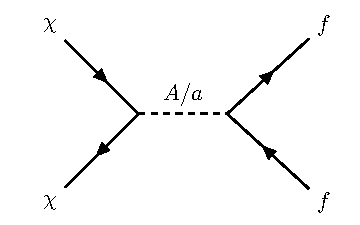
\includegraphics[width=0.35\textwidth]{texinputs/05_relic/figures/feynman/graph_2hdm_relic_s_fermions.pdf}
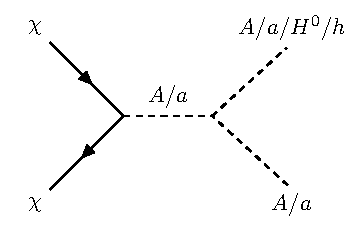
\includegraphics[width=0.35\textwidth]{texinputs/05_relic/figures/feynman/graph_2hdm_relic_s_bosons.pdf}
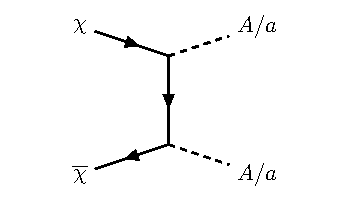
\includegraphics[width=0.35\textwidth]{texinputs/05_relic/figures/feynman/graph_2hdm_relic_ss_bosons.pdf}
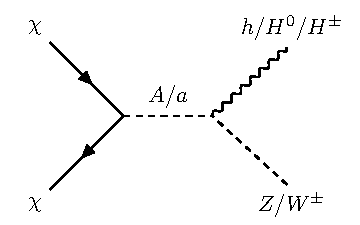
\includegraphics[width=0.35\textwidth]{texinputs/05_relic/figures/feynman/graph_2hdm_relic_s_vbosons.pdf}

\caption{Annihilation diagrams taken into account in the relic density calculation.}
\label{fig:feyn_annihilation}
\end{figure}

The \maddm~\cite{Backovic:2013dpa,Backovic:2015cra} plugin for \mgamcnlo is used to calculate the present-day relic density for this model.
%By modeling the thermal evolution of the cross-section during the expansion of the early universe, the time of freeze-out is determined.
All tree-level annihilation processes are taken into account, and the Yukawa couplings of all fermions are taken to be non-zero.
The Feynman diagrams of annihilation processes taken into account in this calculation are shown in \autoref{fig:feyn_annihilation}. Generally, the annihilation proceeds via single or double s-channel exchange of the pseudoscalars $a$ and $A$, with subsequent decays. Since \maddm uses only tree-level diagrams, contributions from off-shell pseudoscalars can only be taken into account for the case of single s-channel mediation with direct decay of the pseudoscalars to SM fermions. If the pseudoscalars instead decays to other bosons or if the annihilation proceeds through double s-channel diagrams, the outgoing bosons are taken to be on-shell and their decays are not simulated. 

Following \autoref{sec:ParameterScan}, we use the parameter choices $sin(\theta)=0.35$, $m_{h} = 125 GeV$, $g_{\chi}=1$, $\lambda_i = 3$ for all scans in this section.

\subsection{Results}

\begin{figure}[h]
\centering
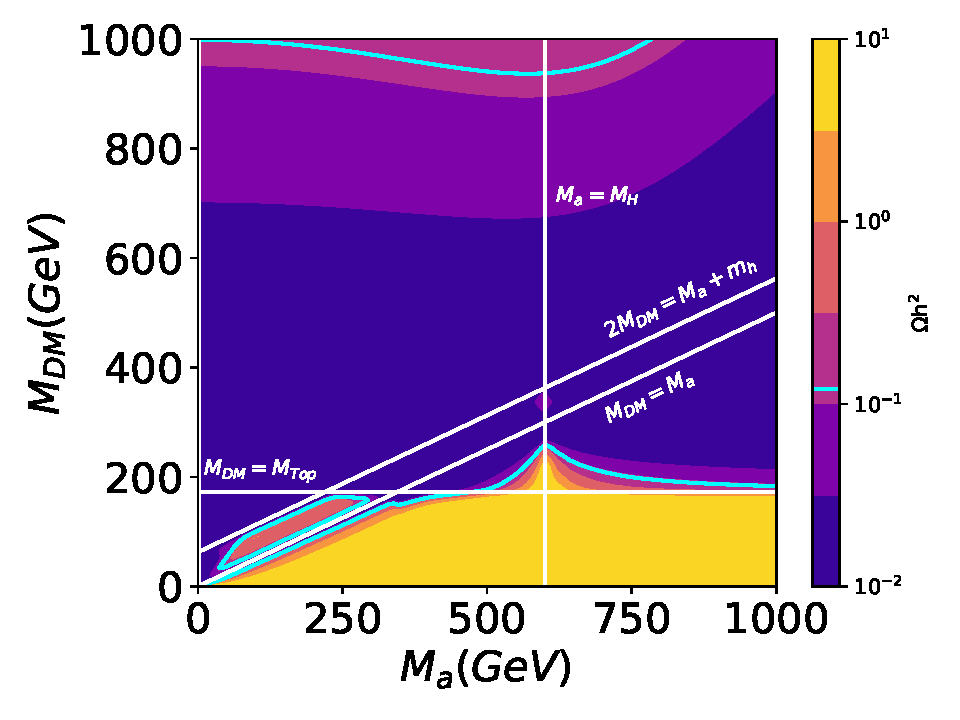
\includegraphics[width=0.49\textwidth]{{texinputs/05_relic/figures/relic/contour_scan_mxd_ma.pdf}}
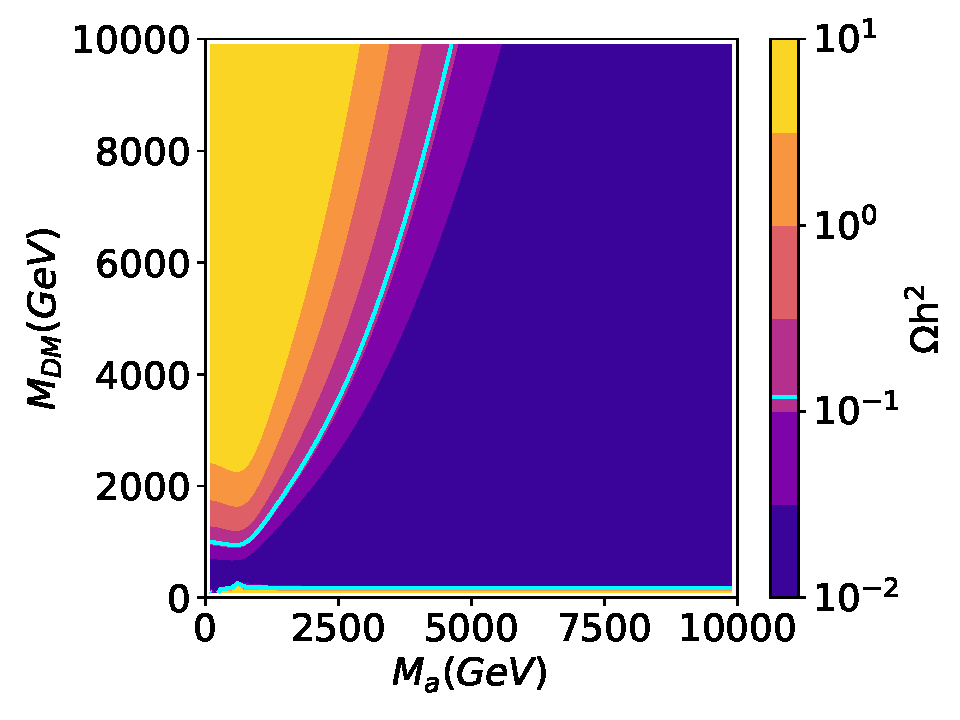
\includegraphics[width=0.49\textwidth]{{texinputs/05_relic/figures/relic/contour_scan_mxd_ma_large.pdf}}
\caption{Predicted relic density for a two-dimensional scan of \mDM and \ma. The other parameters of the model remain fixed with $m_{H}=m_{A}=m_{H^{\pm}}=\unit[600]{GeV}$ and $\tanb=1$, as well as the default choices described in the text. The color scale indicates the relic density, the cyan solid line shows the observed value of $\Omega h^{2} = 0.12$. The color scale is truncated at its ends, i.e. values larger than the maximum or smaller than the minimum are shown in the same color as the maximum/minimum. While the left focuses on the mass region relevant to collider searches, the right panel shows the development of the relic density for a larger mass region.}
\label{fig:relic_scan_mxd_ma}
\end{figure}

The relic density is shown for in the \ma-\mDM plane in \autoref{fig:relic_scan_mxd_ma}.
For small values of $\mDM$ below the mass of the top quark, DM is mostly overabundant. 
In this regime, annihilation to quarks is suppressed by the small Yukawa couplings of the light fermions. 
The observed relic density can only be achieved for $\mDM\approx\ma/2$, where annihilation is resonantly enhanced, or for $\mDM \approx (\ma+\mh)/2$, close to the threshold for the $\chi\chi\rightarrow h a$ process.
Above the top threshold, annihilation into fermions becomes very efficient and DM is underabundant. 
As \mDM increases further, annihilation via single s-channel diagrams is increasingly suppressed and the relic density rises again. 
The observed density is produced by this model for $\mDM\approx1 \mathrm{TeV}$ at low \ma.
\textbf{[The following sentence is being checked with Andreas Albert - would remove]} For values of \ma beyond the LHC reach of a few TeV, the allowed parameter region at the top threshold $\mDM\approx m_{\mathrm{top}}$ remains independent of the value of \ma, indicating that a DM candidate that is mass degenerate with the top quark cannot be excluded by LHC searches alone.

\begin{figure}[h]
\centering
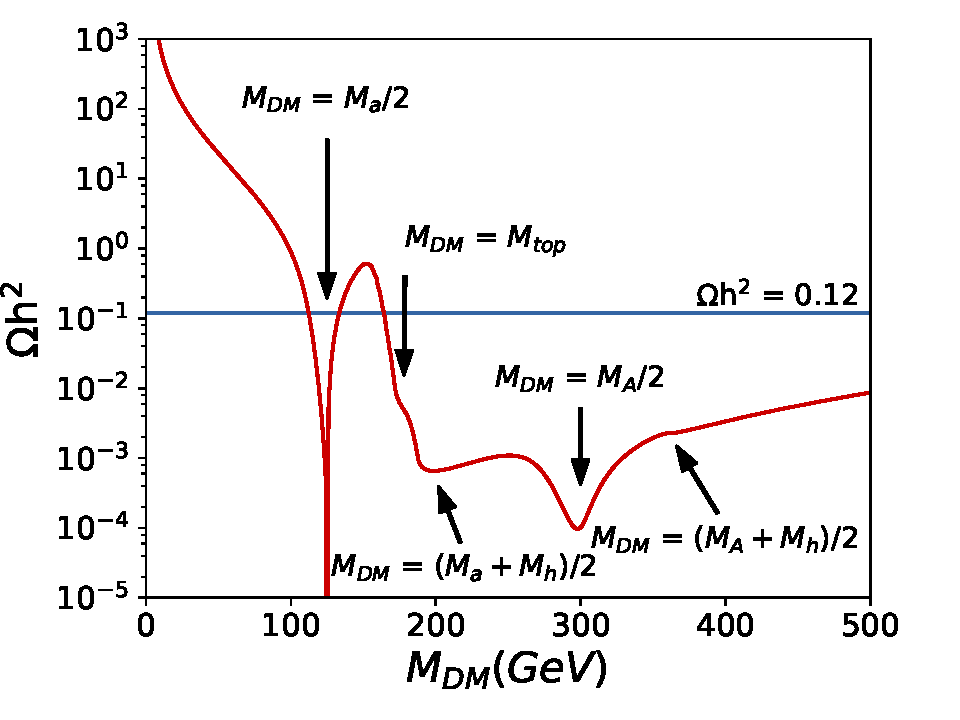
\includegraphics[width=0.8\textwidth]{texinputs/05_relic/figures/relic/line_scan_mdm.pdf}
\caption{Relic density for a one-dimensional scan of \mDM. The other parameters of the model remain fixed with $m_{H}=m_{A}=m_{H^{\pm}}=\unit[600]{GeV}$, $\ma=\unit[250]{GeV}$ and $\tanb=1$, as well as the default choices described in the text. Various kinematic thresholds and regions of resonant enhancement are visible. Consistency with the observed value of $\Omega h^{2} = 0.12$ is mainly controlled by the resonant enhancement of $\chi\chi\rightarrow a$, as well as the onset of $\chi\chi\rightarrow t\overline{t}$.}
\label{fig:relic_scan_mxd}
\end{figure}

The dependence of the relic density on the choice of \mDM is further explored by performing a one-dimensional scan as a function of the DM mass fixing \mH = \mA = $m_{H^{\pm}}$ = 600GeV, \ma = 250GeV, and shown in \autoref{fig:relic_scan_mxd}. 
The relic density confirms structures corresponding to the previously discussed regions of resonant enhancement and to the kinematic boundaries. 
Overall, the behavior is dominated by the low-\mDM suppression of the annihilation cross-section, the resonant enhancement at $\mDM = \ma/2$ and the kinematic top thresholds. 
Other effects, such as the resonant enhancement of $\chi\chi\rightarrow A$ annihilation are present, but only have small effects. 

\begin{figure}[h]
\centering
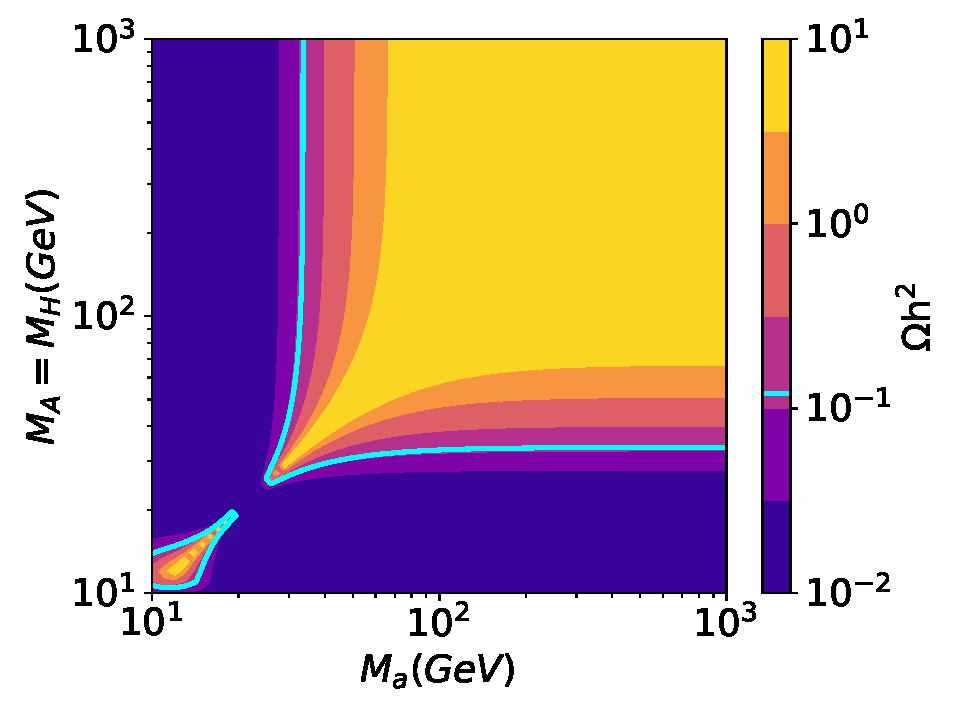
\includegraphics[width=0.49\textwidth]{{texinputs/05_relic/figures/relic/contour_scan_mA_ma_mxd10.pdf}}
\caption{Predicted relic density for a two-dimensional scan of \ma and $\mA=\mH=\mHc$. The other parameters of the model remain fixed with $\mDM=\unit[10]{GeV}$, $\tanb=1$, \mH = \mA = $m_{H^{\pm}}$. The color coding is identical to Fig.~\ref{fig:relic_scan_mxd_ma}.}
\label{fig:relic_scan_mA_ma}
\end{figure}

The relic density values for the \ma-\mA/\mH scan described in \autoref{sec:ParameterScan} is shown in \autoref{fig:relic_scan_mA_ma}. 
For the model parameters chosen in this whitepaper, the regions where the model generates a relic density compatible with the measured value are located at relatively small values of $\ma < \unit[30]{GeV}$ or $\mA=\mH=\mHc < \unit[30]{GeV}$, which are already excluded by LHC and LEP searches (see section 4 of Ref.~\cite{Bauer:2017ota}). 
The cosmological production of DM is largely driven by the choice of $\mDM$. As shown in \autoref{subsub:mDMKinematics}, the model kinematics is largely insensitive to this choice if $\mDM < 2 \ma$. Future experimental results that are sensitive to DM masses around 100 GeV which can yield the measured relic density can still be interpreted by rescaling samples generated according to this parameter scan. 

The $\tanb$-dependent scans, as a function of \ma and \mDM, are shown in Fig.~\ref{fig:relic_scan_mass_tanbeta}. The choice of \tanb acts as an overall modifier of the annihilation cross-section and thus the relic density, and the effect is largely independent of the choice of $\ma$ and $\mDM$. For a choice of $\tanb\approx0.6$, the relic density becomes maximal and steadily decreases for larger and smaller values of \tanb. In the $\mDM$ dependent scan, where \ma is fixed to 250 GeV, the reduction of the relic density at low ($\approx0.1$) and high ($\approx3$) values of $\tanb$ leads to the disappearance of the overabundant island around $\mDM\approx\ma/2$.

\begin{figure}[h]
\centering
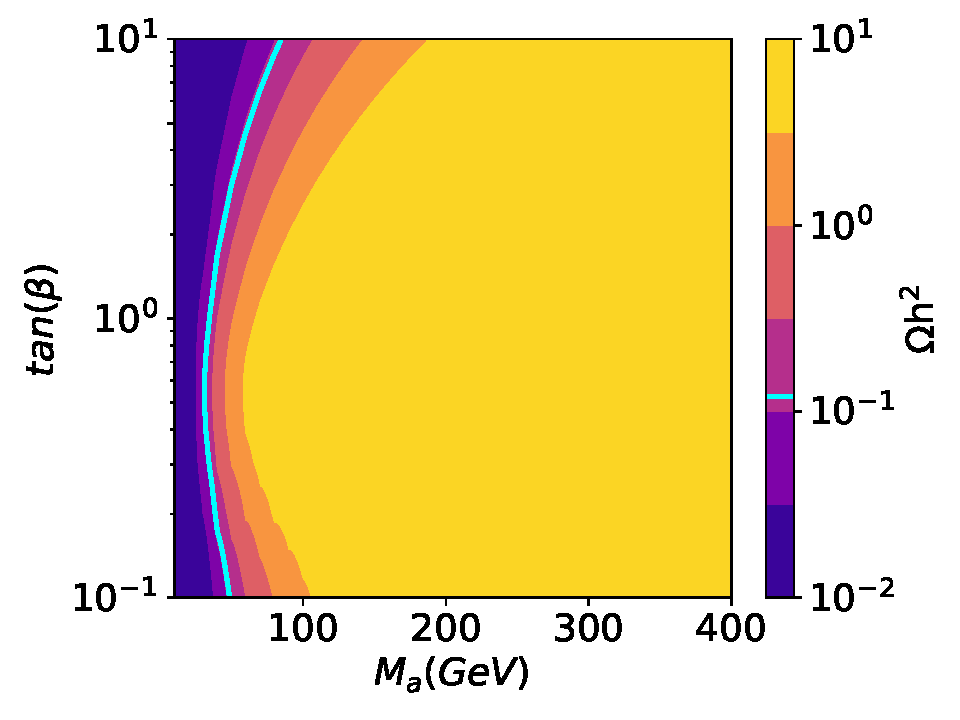
\includegraphics[width=0.49\textwidth]{{texinputs/05_relic/figures/relic/contour_scan_ma_tanbeta.pdf}}
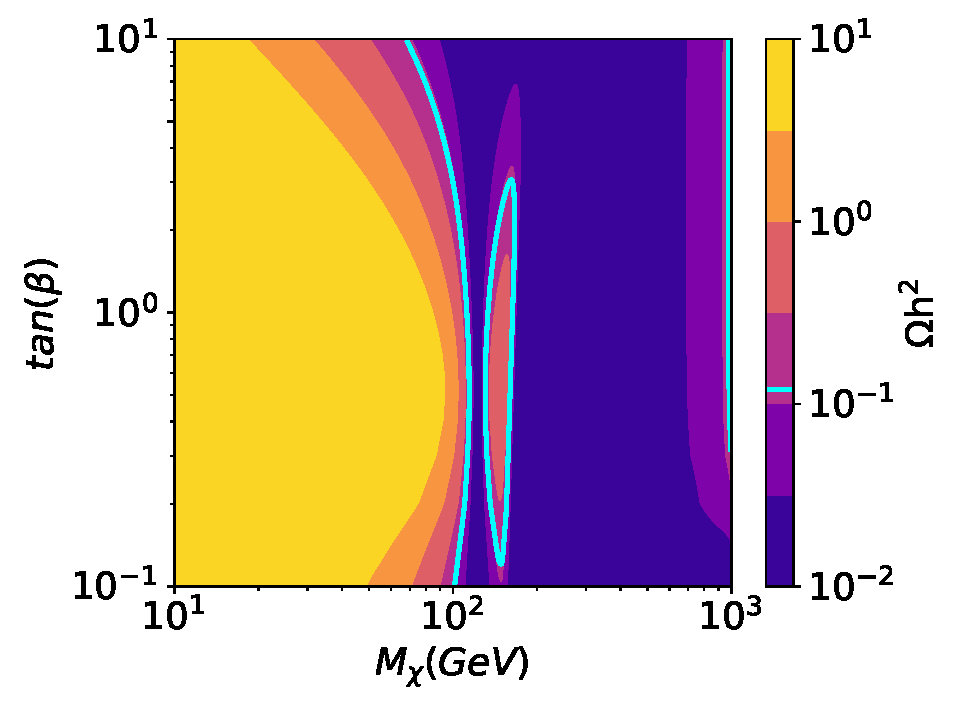
\includegraphics[width=0.49\textwidth]{{texinputs/05_relic/figures/relic/contour_scan_mxd_tanbeta.pdf}}
\caption{Predicted relic density for a two-dimensional scan of \tanb and \ma (left), \mDM (right). In the case of the \mDM ($\ma$) dependent scan, $\ma=\unit[250]{GeV}$ ($\mDM=\unit[10]{GeV}$) is used. The other parameters of the model remain fixed with $m_{H}=m_{A}=m_{H^{\pm}}=\unit[600]{GeV}$, as well as the default choices described in the text. The color coding is identical to Fig.~\ref{fig:relic_scan_mxd_ma}.}
\label{fig:relic_scan_mass_tanbeta}
\end{figure}

%\subsection{Scalar}
%
%\begin{figure}
%    \centering
%    \hspace{2em} 
%    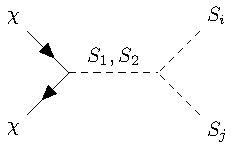
\includegraphics{texinputs/05_relic/figures/relic_scalar/XXSS.pdf} \hspace{3em} \vspace{2em} 
%    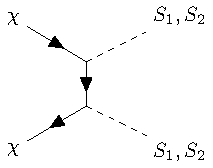
\includegraphics{texinputs/05_relic/figures/relic_scalar/XXSSt.pdf} \hspace{3em} 
%    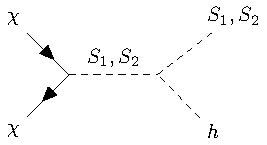
\includegraphics{texinputs/05_relic/figures/relic_scalar/XXSh.pdf}  \hspace{0.5em} \\ 
%    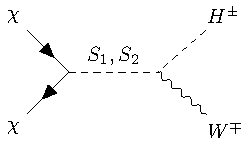
\includegraphics{texinputs/05_relic/figures/relic_scalar/XXWH.pdf} \hspace{2em} 
%    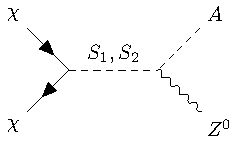
\includegraphics{texinputs/05_relic/figures/relic_scalar/XXZA.pdf} \hspace{2em} 
%    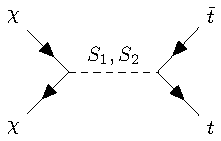
\includegraphics{texinputs/05_relic/figures/relic_scalar/XXtt.pdf} 
%    \caption{Dominant DM annihilation channels, where $(S_i,S_j)$ is one of these scalar final states: $(S_1,S_1)$, $ (S_1,S_2)$, $(S_2,S_2)$, $(H^+,H^-)$, $(A,A)$.}
%    \label{fig:feyn}
%\end{figure}
%
%The 2HDM+S scenario has multiple DM annihilation channels.
%There are tree-level annihilations to fermion-antifermion pairs,
%scalars (the SM Higgs, the two neutral scalars, the pseudoscalar, and the
%charged scalars) and/or the electroweak gauge bosons,
%namely: $\overline{\chi}\chi \rightarrow \overline{f}f$, $S_1 S_1$, $S_2
%S_2$, $S_1 S_2$, $H^+ H^-$, $H^+ W^-$, $A A$, $A Z$, $S_1 h$, and $S_2
%h$ -- these are shown in Fig.~\ref{fig:feyn}. This is to be compared with a single mediator model in which only
%the $\overline{f}f$ and $SS$ channels are present. Note that since all
%diagrams involve $\chi$-scalar vertices (including those with gauge
%boson final states) they are all $p$-wave processes. As such, while we
%will easily be able to find parameters that accommodate the observed
%relic density, there will be no constraints arising from indirect
%detection because the $p$-wave annihilation processes are highly velocity
%suppressed in the late universe.
%
%
%If the DM particle is relatively light, such that annihilation to the
%scalars and electroweak bosons is kinematically forbidden ($m_\chi \lesssim
%80\GeV$), the only annihilation channels that remain open are the
%fermionic ones.  This case is heavily constrained, as the dominant
%annihilation channel is then $b\bar{b}$, which is suppressed by the
%bottom Yukawa coupling and thus usually requires resonant enhancement
%to accommodate the correct relic density.
%
%
%If, instead, the DM particle is heavy enough to annihilate to the Higgs,
%electroweak gauge bosons and/or the new scalars, then these final states will
%likely dominate due to the Yukawa suppression of annihilations to fermions 
%(top excluded).
%Because all of these annihilations are governed by scalar and electroweak
%couplings -- and exist due to gauge invariance, independent of the
%Yukawa couplings of the second doublet -- they are also present,
%for example, in the limit where the second doublet is inert.
%This ability to produce the correct relic abundance independent of
%Yukawa structure means that DM can be adequately produced while
%avoiding any Yukawa dependent constraints (e.g. DD, neutral meson
%mixing, $b \to s \gamma$, $\mu \to e \gamma$, etc.).
%
%%%%%%%%%%%%%%%%%%%%%%%%%%%%%%%%%%%%%%%%%%%
%\begin{figure}[t]
%\centering
%\begin{subfigure}[t]{0.43\textwidth}
%\includegraphics[width=\textwidth]{texinputs/05_relic/figures/relic_scalar/mDM_yDM4.pdf}
%\label{fig:scan1a}
%\end{subfigure}
%\hspace{1em}
%\begin{subfigure}[t]{0.43\textwidth}
%\includegraphics[width=\textwidth]{texinputs/05_relic/figures/relic_scalar/MS1_Theta2.pdf}
%\label{fig:scan1b}
%%\caption{\centering Second Higgs and scalar singlet mixing angle versus DM mass. The plot is symmetric across $| \theta | = \pi / 2$ if extended.}
%\end{subfigure}
%\vspace{0.5ex}
%\begin{subfigure}[t]{0.43\textwidth}
%\includegraphics[width=\textwidth]{texinputs/05_relic/figures/relic_scalar/MS1_mDM3.pdf}
%%\caption{DM mass - lighter scalar mass plane $m_\chi - M_{S_1}$.}
%\label{fig:scan1c}
%%\caption{\centering Two additional neutral scalar masses. Note that we have chosen $M_{S_2} > M_{S_1}$; if this is relaxed, then the plot is simply symmetric across the solid black line.}
%\end{subfigure}
%\hspace{1em}
%\begin{subfigure}[t]{0.43\textwidth}
%\includegraphics[width=\textwidth]{texinputs/05_relic/figures/relic_scalar/MS2_mDM3.pdf}
%%\caption{DM mass - heavier scalar mass plane $m_\chi - M_{S_2}$.}
%\label{fig:scan1d}
%%\caption{\centering DM mass versus lightest new scalar mass eigenstate.}
%\end{subfigure}\\
%\begin{subfigure}[t]{0.86\textwidth}
%\includegraphics[width=\textwidth]{texinputs/05_relic/figures/relic_scalar/LegendH2.pdf}
%\end{subfigure}
%\caption{Points of our scan of parameter space that produce the correct relic density. The colours represent the dominant annihilation channel, as shown above. 15000 points are taken that survive the constraints, and of them only 25\% of the $H^+H^-$ channel and 10\% of the $S_1S_1$ channel are shown for clarity. The black line in the lower panels indicate $m_\chi = 2 M_{S_1, S_2}$, which is the resonance condition for the s-channel annihilation processes. The blue line in the top left panel represents the scaling expected for a cross section of $\langle \sigma v \rangle \sim y^4_\chi v^2 / 16 \pi^4 m_\chi^2$ which, in this model, applies to a pure $\overline{\chi}\chi \to S_iS_i$ scenario.}
%\label{fig:scan1}
%\end{figure}
%%%%%%%%%%%%%%%%%%%%%%%%%%%%%%%%%%%%%%%%%%%
%
%We implemented the model in Feynrules\footnote{The Feynrules model file used is publicly available in the Feynrules model database.} \citep{Christensen:2008py,Alloul:2013bka} and output the model with the CALCHEP interface~\citep{Christensen:2009jx}. We then used {\tt micrOMEGAs}~\citep{Barducci:2016pcb} to perform the relic density calculation, where we included 3 body final states with off-shell gauge bosons. We also double checked the results by calculating the annihilation cross sections, which are reported in \citep{Bell:2017rgi}. In the case where the parameter values are away from resonances and annihilation thresholds, one can use the wave expansion of the cross sections. The p-wave coefficients of this expansion are also reported in \citep{Bell:2017rgi}.
%
%Sommerfeld enhancement can significantly increase the DM annihilation
%cross section~\citep{Feng:2010zp,Cassel:2009wt,Iengo:2009ni}, provided
%at least one of the scalars is both sufficiently light compared to the
%DM, and strongly coupled to the DM particle.  In practice, for the
%parameter range we consider, this leads to $\mathcal{O}(1)$
%corrections to the cross section; a discussion is provided in
%\citep{Bell:2017rgi}.
%
%%%%%%%%%%%%%%%%%%%%%%%%%%%%%%%%%%%%%%%%%%%
%\begin{figure}[ht]
%\centering
%\begin{subfigure}[t]{0.45\textwidth}
%\includegraphics[width=\textwidth]{texinputs/05_relic/figures/relic_scalar/MS1_MS25.pdf}
%%\caption{Heavier - lighter scalar mass plane $M_{S_2} - M_{S_1}$.}
%\label{fig:scan1e}
%%\caption{\centering DM mass versus lightest new scalar mass eigenstate.}
%\end{subfigure}
%\hspace{1em}
%\begin{subfigure}[t]{0.45\textwidth}
%\includegraphics[width=\textwidth]{texinputs/05_relic/figures/relic_scalar/mDM_Lambda4.pdf}
%%\caption{$\Lambda$ versus $m_\chi$}
%\label{fig:scan1f}
%%\caption{\centering DM mass versus lightest new scalar mass eigenstate.}
%\end{subfigure}
%\begin{subfigure}[t]{0.9\textwidth}
%\includegraphics[width=\textwidth]{texinputs/05_relic/figures/relic_scalar/LegendH2.pdf}
%\end{subfigure}
%\caption{Points of our scan of parameter space that produce the correct relic density. The colours represent the dominant annihilation channel, as shown above. 15000 points are taken that survive the constraints, and of them only 25\% of the $H^+H^-$ channel and 10\% of the $S_1S_1$ channel are shown for clarity. $\Lambda$ is the effective cut-off scale for the DD effective operator; the dotted orange line represents the constraint from the LUX 2016 results \citep{Akerib:2016vxi}, the solid blue represents the XENON1T experiment \citep{Aprile:2017iyp}, the dashed blue the projection for the XENON1T experiment with $2t\cdot y$ of data taking, the dotted blue the projection for the XENONnT experiment with $20t\cdot y$ of data taking \citep{Aprile:2015uzo}, and the magenta is the DD sensitivity at the ``neutrino floor''\citep{Billard:2013qya}.}
%\label{fig:scan11}
%\end{figure}
%
%The independent parameters present in the model are
%\be
%m_\chi, \quad M_{S_1}, \quad M_{S_2}, \quad y_\chi, \quad \hat{\lambda}_4, \quad \hat{\lambda}_5, \quad \hat{\lambda}_{hHS}, \quad \hat{\lambda}_{HHS}, \quad \epsilon_u \quad \textrm{and} \quad \epsilon_d.
%\ee
%This set of parameters, through the minima condition and the diagonalization relations, together with the additional constraint $m_\chi = y_\chi v_s$, determine all other parameters of the model\footnote{The phase of the DM Yukawa can always be reabsorbed, so one can chose $y_\chi$ and $v_s$ to be both real and positive.}.
%%
%The scan is performed in the following range:
%\bea
%70\GeV < &m_\chi& < 1\TeV,\\
%70\GeV < &M_{S_1}& < M_{S_2} < 2 \TeV, \\
%0 < &y_\chi& < 2,\\
%&|\hat{\lambda}_{hHS}|& < 2,\\
%&|\hat{\lambda}_{HHS}|& < 4,\\
%0 < &\epsilon_u& < 1,
%\eea
%while for $\hat{\lambda}_4$ and $\hat{\lambda}_5$ we scan over the region shown in \citep{Bell:2017rgi}. 
%These ranges for the couplings were chosen so that most of the points will satisfy unitarity and perturbativity bounds, which was checked via the scalar scattering matrices as in \citep{Bell:2016ekl}.
%To achieve the right relic density, we will see that it will be in general necessary to have $m_\chi\gtrsim M_{S_1}$, and the inequality is strictly required for DM masses below the top mass, as otherwise all considered annihilation channels are closed. In this low DM mass region, however, one needs to take into account Higgs invisible constraints \citep{Aad:2015pla,Khachatryan:2016whc}: 2-body decays forbid the region $2m_\chi<m_h$ and $2M_{S_1}<m_h$, while considering 3-body decays as well further pushes up the lower bound on $M_{S_1}$ to nearly $100\GeV$. The Higgs invisible decays constraints can only be avoided in the $\theta\rightarrow\pi/2$ limit, but in such case the model approaches a decoupled dark sector which is phenomenologically uninteresting\footnote{Relic density requirement can be satisfied in the limit of a decoupled dark sector, in which dark matter annihilates to light dark scalars. However, there would be no signals in collider or direct detection experiments. Moreover, indirect detection is prevented by the p-wave nature of annihilation to scalars, even if small couplings to the SM are included.}. Taking into account these considerations, we have chosen in our scan a conservative lower bound for the DM mass and for the lightest scalar of $70\GeV$.
%Points are selected if they have a relic density between $0.1 < \Omega h^2 < 0.14$ and satisfy all bounds from flavour, unitarity, perturbativity, tree level vacuum stability, and DD constraints. 
%
%\begin{figure}
%\begin{center}
%%\vspace*{1.5cm} 
%\includegraphics[width=0.7\textwidth]{texinputs/05_relic/figures/relic_scalar/RelicPlot.pdf}
%\caption{One-dimensional scan of the parameter space. We fix all other parameters, see the text for more details.} 
%\label{fig:scalarrelic1D}
%\end{center}
%\end{figure}
%
%The relic density is insensitive to the value of $\epsilon_d$, while the DD results depend on the relationship $\epsilon_d$ and $\epsilon_u$.  
%We set $\epsilon_d = \epsilon_u$ for the scans presented in Fig.~\ref{fig:scan1} and Fig.~\ref{fig:scan11} (with the exception of the right panel of Fig.~\ref{fig:scan11}, which enforces no DD constraint and hence has no $\epsilon_d$ dependence). 
%
%We have chosen to define $S_1$ to be the lighter of the 2 scalars, and allow $\theta$ to range from $0$ to $\pi/2$. As one can always switch the two scalars by sending $\theta\rightarrow\pi/2-\theta$, an equivalent choice would be to take $0<\theta<\pi/4$ without requiring any mass ordering.
%
%In Fig. \ref{fig:scalarrelic1D} we show the value of the relic density obtained through thermal freezeout in a one-dimensional scan, where we kept fixed all parameters except the DM mass. We fix $M_{S_1}=250\GeV$, $M_{S_2}=M_A=M_{H^+}=600\GeV$, $\cos\theta=0.35$ (equivalent to $\sin\theta=0.35$ for the PS model), $y_\chi=1$, 
%
%
%These choices of parameters, along with alignment conditions and $m_\chi = v_s y_\chi$, then fix
%\begin{align}
%    v_s &= \frac{m_\chi}{y_\chi} = m_\chi, \\
%    \lambda_1 &= \frac{m_h^2}{v^2} \sim 0.258, \\
%    \lambda_{s} &= \frac{1}{4 v_s^2} \left( M_{a}^2 + M_A^2 +(M_A^2 - M_a^2) \cos (2\theta ) \right) \sim \frac{222.4^2\GeV^2}{m_\chi^2}, \\
%%    \lambda_{11s} &= 0, \\
%    \lambda_{12s} &= \frac{(M_{S_1}^2 - M_{S_2}^2) \sin (2\theta)}{2 v v_s} \sim -\frac{396.5 \GeV}{m_\chi},\\
%    \lambda_4 &= \frac{1}{2v^2} \left( 2 M_{A}^2 - 4 M_{H^+}^2 + M_{S_1}^2 + M_{S_2}^2 + (M_{S_1}^2 - M_{S_2}^2) \cos (2 \theta ) \right) \sim -0.60, \\
%    \lambda_5 &= -\frac{1}{2v^2} \left( 2 M_{A}^2 - M_{S_1}^2 - M_{S_2}^2 + (M_{S_2}^2 - M_{S_1}^2) \cos (2 \theta ) \right) \sim -0.60, \\
%    \lambda_3 &= \lambda_1 - \lambda_4 - \lambda_5 \sim  1.46.
%\end{align}
%


\section{Comparisons with non-collider experiments}
\subsection{Direct detection}
\subsection{Direct Detection}

The DD constraints for the scalar and pseudoscalar mediator scenario are very different. While the scalar features an unsuppressed SI scattering cross section, the pseudoscalar cross section is highly suppressed at tree level such that the dominant contribution arises from loop graphs.

\subsubsection{Scalar}

We will generate DD constraints using the 2016 LUX~\citep{Akerib:2016vxi} and XENON1T~\citep{Aprile:2017iyp} data, via an effective operator approach using tools from \citep{DelNobile:2013sia}. The scattering of DM with nuclei will be dominated by the tree-level exchange of $S_1$ and $S_2$, resulting in a spin-independent scattering cross section. The only relevant nucleon operator is
\begin{align}
O_1^N = \bar{\chi} \chi \bar{N} N,  
\end{align}
and, by integrating out the mediators, we obtain a coefficient of \citep{Bell:2016ekl}
\begin{align}
c_N = m_N\frac{y_\chi \cos\theta\sin\theta}{v}\left(\frac{1}{M_{S_1}^2}-\frac{1}{M_{S_2}^2}\right) \left(f_{T_u}^N\epsilon_u + \epsilon_d\sum_{q=d,s} f_{T_q}^N + \frac{2}{9} f_{T_g} \frac{2 \epsilon_u+ \epsilon_d}{3} \right).
\label{eq:DDcoeff}
\end{align}

As there are contributions from exchange of the two scalars, with a relative negative sign, there is the possibility for destructive interference when the masses of $S_1$ and $S_2$ are comparable. 
%
In addition, depending on the choice of Yukawa structure, it is possible to have destructive interference between the up-type quarks and the down-type quarks in the nucleon. For the Type I and Type II Yukawa structure, the coefficients become
%
\small
\bea
c_N^{\text{type I}} &=&  m_N\frac{y_\chi \cos\theta\sin\theta}{v\tan\beta}\left(\frac{1}{M_{S_1}^2}-\frac{1}{M_{S_2}^2}\right) \left(\sum_{q=u,d,s} f_{T_q}^N  + \frac{2}{9} f_{T_g} \right),\\
c_N^{\text{type II}} &=&  m_N\frac{y_\chi \cos\theta\sin\theta}{v}\left(\frac{1}{M_{S_1}^2}-\frac{1}{M_{S_2}^2}\right) \left(f_{T_u}^N\cot\beta - \tan\beta\sum_{q=d,s} f_{T_q}^N + \frac{2}{9} f_{T_g} \frac{2\cot\beta-\tan\beta}{3} \right),
\label{scalarDD_typeII}
\eea
\normalsize
%
For the Type II scenario, we see that the presence of destructive $u$-$d$ interference is clearly visible in the right-hand bracket of \ref{scalarDD_typeII}. There is no such interference for Type I. If we adopt the values of $f_{T_i}$ obtained by~\citep{Gondolo:2004sc}, we find that a ratio of $\epsilon_u \sim - 1.6 \epsilon_d$ (corresponding to $\tan\beta=\sqrt{|\frac{\epsilon_d}{\epsilon_u}|}\sim 0.8$ in a Type II scenario) will result in exact cancellation of the DD signal.


In Figure~\ref{fig:SDD} we show the current DD exclusion from LUX \citep{Akerib:2016vxi} and XENON1T\citep{Aprile:2017iyp} together with the projections for XENON1T, XENONnT projections \citep{Aprile:2015uzo}.  We also show the sensitivity for a cross section equivalent to the ``neutrino floor" \citep{Billard:2013qya}.  We find that DD excludes significant parameter space, unless the scalar masses are approximately degenerate.  This can be seen in all 4 panels of Figure~\ref{fig:SDD} where we see a narrow allowed region near $M_{S_1} \sim M_{S_2}$, between excluded regions at higher and lower $M_{S_1}$ values.  
The excluded region in the upper LH plot (Type I) is somewhat larger than in the lower LH plot (Type II) lower due to the additional interference effect for the latter.
Increasing $\tan\beta$ weakens the constraints for Type I because $|\epsilon_d|=|\epsilon_u|=1/\tan\beta$ (upper right) and strengthens them for Type II because $|\epsilon_d|=|1/\epsilon_u|=\tan\beta$ (lower right).



%%%%%%%%%%%%%%%%%%%%%%%%%%%%%%%%%%%%%%%%%%%%%%%%%%%%%%%%%%%
\begin{figure}[ht]
\begin{center}
\includegraphics[width=0.49\textwidth]{texinputs/06_comparisons/figures/S_TI_TB1.pdf}
\includegraphics[width=0.49\textwidth]{texinputs/06_comparisons/figures/S_TI_TB5.pdf}\\
\includegraphics[width=0.49\textwidth]{texinputs/06_comparisons/figures/S_TII_TB1.pdf}
\includegraphics[width=0.49\textwidth]{texinputs/06_comparisons/figures/S_TII_TB3.pdf}
\caption{DD exclusion and projections for various experiments for the Scalar model. The various regions refer, in order, to LUX \citep{Akerib:2016vxi}, XENON1T\citep{Aprile:2017iyp}, XENON1T and XENONnT projections \citep{Aprile:2015uzo}, and neutrino background \citep{Billard:2013qya}. The mixing angle is set to $\sin\theta=0.35$, but results are equivalent also for $\cos\theta=0.35$, while $M_{S_2}=750\GeV$ in all the panels.} 
\label{fig:SDD}
\end{center}
\end{figure} 
%%%%%%%%%%%%%%%%%%%%%%%%%%%%%%%%%%%%%%%%%%%%%%%%%%%%%%%%%%%

\subsection{Pseudoscalar}

\begin{figure}[ht]
    \centering
    \includegraphics[width=0.3\textwidth]{texinputs/06_comparisons/figures/pseudoTriangle.pdf} \hspace{0.02\textwidth}
    \includegraphics[width=0.3\textwidth]{texinputs/06_comparisons/figures/pseudoBox.pdf} \hspace{0.02\textwidth}
    \includegraphics[width=0.3\textwidth]{texinputs/06_comparisons/figures/pseudoBox2.pdf} 
    \caption{Spin-independent DM-nucleon scattering arises from the loop exchange of the mixing pseudoscalar mediators. Left panel: triangle diagrams. Central and right panel: box diagrams.}
    \label{fig:feynDDPS}
\end{figure}



At tree level, the spin-independent scattering cross section is absent. The spin-independent cross section is non-zero, but highly suppressed due to a dependence on $q_{tr}^4$. At loop level, however, a spin-independent cross section is generated through the diagrams in Fig. \ref{fig:feynDDPS}. 
The triangle diagrams in the left panel of Fig. \ref{fig:feynDDPS} are proportional to $m_q$ while the box diagrams in the central and right panels of Fig. \ref{fig:feynDDPS} are proportional to $m_q^3$, thus the box diagrams are sub-leading as found in \citep{Ipek:2014gua} (except for Type II with $\tan\beta\gtrsim50$).
The triangle diagram does not depend on the Yukawa sector of the 2HDM. ** cite our paper in preparation**

Similarly as in the scalar model, in the PS model the mixing arises through a term $i b_P P \Phi_1^\dagger \Phi_2 +h.c.$. The resulting mixing angle is defined by

\begin{equation}
    b_P = -\frac{(M_A^2-M_a^2)\sin2\theta}{2v}
\end{equation}

%*** define $\sin 2\theta$  in terms of $\mu_{12s}$ somewhere ***\\
%*** also define $\lambda_{34-5}$ ***\\
%*** remove discussion of why  \citep{Ipek:2014gua} is wrong ***


The low energy effective operator generated at 1 loop is%in the approximation $M_{A}\gg M_{a}$ (in which case one considers only the diagram with two $a$'s appearing in the loop) is
\begin{eqnarray}
\mathcal{L}_{eff} &=& - \frac{y_\chi^2 m_q m_\chi}{16\pi^2 m_h^2 v^2}     G\left(\frac{m_\chi^2}{M_{A}^2},\frac{m_\chi^2}{M_{a}^2},\frac{m_h^2}{m_\chi^2},\theta\right) \bar{\chi}\chi\bar{q}q\label{eq:loopps}\\
G\left(x,y,z,\theta\right) &=& F_1(x)\sin^2\theta\hat{\mu}_{AAh}+F_1(y)\cos^2\theta\hat{\mu}_{aah}+F_2(x,y)\sin2\theta\hat{\mu}_{Aah}\label{eq:f2}\\
F_1(x) &=& \int_0^1 dz \frac{x (1-z) z}{x z^2-z+1} = \frac{(6 x-2) \log \left(\frac{\sqrt{1-4 x}+1}{2 \sqrt{x}}\right)+\sqrt{1-4 x} ((x-1) \log (x)-2 x)}{2 \sqrt{1-4 x} x}\label{eq:f1}\\
F_2\left(x,y\right) &=& \int_0^1 dz \frac{x y z \log \left(\frac{x y z^2-y z+y}{x y z^2-x z+x}\right)}{y-x} \nonumber\\
= \frac{1}{4xy(x-y)} &\bigg(&x^2 ((2 y-1) \log (y)-2 y)+x^2 \sqrt{1-4 y} \left(\log (4 y)-2 \log \left(\sqrt{1-4 y}+1\right)\right) \\
&-&2 x y^2 (\log (x)-1)+y^2 \log (x)+\sqrt{1-4 x} y^2\left(2 \log \left(\sqrt{1-4 x}+1\right)-\log (4 x)\right) \bigg)
%&=&\frac{x^2 ((2 y-1) \log (y)-2 y)+x^2 \sqrt{1-4 y} \left(\log (4 y)-2 \log \left(\sqrt{1-4 y}+1\right)\right)-2 x y^2 (\log (x)-1)+y^2 \log (x)+\sqrt{1-4 x} y^2\left(2 \log \left(\sqrt{1-4 x}+1\right)-\log (4 x)\right)}{4 x y (x-y)}\label{eq:f3}
\end{eqnarray}
%Our result differs from the one found in \citep{Ipek:2014gua} because of two reasons. First, we find that the amplitude contains an additional $\cos^2\theta$ factor, coming from the $\bar{\chi}\chi a$ yukawa couplings, on the top of the $\sin^2 2\theta$ factor coming from the cubic scalar vertex $aah$. Second, we find that the cubic scalar vertex $aah$ receives contributions not only from the portal term $\frac{1}{2}(i\mu_{hHP} \Phi_1^\dagger \Phi_2 P + h.c.)$, but also from the 2HDM terms proportional to $\lambda_{3},\lambda_{4}$ and $\lambda_{5}$, as it is manifest in Eq. \ref{eq:mu22h} \comm{add $\lambda_{P,1,2}$}. Depending on the point of the parameter space, these differences can be significant. To reduce the number of free parameters, we will fix $(\hat{\lambda}_3+\hat{\lambda}_4-\hat{\lambda}_5)v^2=\lambda_{34-5}v^2=m_h^2$ through all the section, as a benchmark point.

\begin{figure}[ht]
\begin{center}
\includegraphics[width=0.49\textwidth]{texinputs/06_comparisons/figures/PseudoS07.pdf}
\includegraphics[width=0.49\textwidth]{texinputs/06_comparisons/figures/PseudoS035.pdf}\\
\includegraphics[width=0.49\textwidth]{texinputs/06_comparisons/figures/PseudoC035.pdf}
\caption{DD exclusion and projections for the first benchmark point for various experiments for the Pseudoscalar model. The various regions refer, in order, to LUX \citep{Akerib:2016vxi}, XENON1T\citep{Aprile:2017iyp}, XENON1T and XENONnT projections \citep{Aprile:2015uzo}, and neutrino background \citep{Billard:2013qya}. Top Left panel uses $\sin\theta=0.7$, top right panel uses $\cos\theta=0.35$, bottom panel uses $\cos\theta=0.35$, while $M_A=750\GeV$ in all the panels.} 
\label{fig:PSDD}
\end{center}
\end{figure} 


where the coefficients $\mu$ are given in terms of either the couplings in the $\Phi_{1,2}$ basis or in the $\Phi_{h,H}$ basis (indicated as $\hat{\mu}$), respectively:
\begin{eqnarray}
\mu_{AAh} &=& z\left(\cos^2\theta-\frac{2\lambda_3v^2}{m_h^2}\right), \label{eq:mu11h}\\
\mu_{Aah} &=& -\frac{1}{2}\sin(2\theta)\left(\frac{1}{x}-\frac{1}{y}+z\right),  \label{eq:mu12h}\\
\mu_{aah} &=& 2\sin^2(\theta)\left(\frac{1}{x}-\frac{1}{y}+\frac{z}{2}\right) -z\frac{2\lambda_3 v^2}{m_h^2},\label{eq:mu22h}\\
\hat{\mu}_{AAh} &=& -\frac{1}{2}\sin^2(2\theta)\left(\frac{1}{x}-\frac{1}{y}\right) - z\frac{\hat{\lambda}_{34-5}v^2}{m_h^2}\cos^2\theta -z\frac{2\hat{\lambda}_{P_1}v^2}{m_h^2}\sin^2\theta,  \label{eq:muAAh}\\
\hat{\mu}_{Aah} &=& -\frac{1}{4}\sin(4\theta)\left(\frac{1}{x}-\frac{1}{y}\right) + \frac{z}{2}\frac{(\hat{\lambda}_{345P}-2\hat{\lambda}_{P_1}) v^2}{m_h^2}\sin(2\theta), \label{eq:muaAh}\\
\hat{\mu}_{aah} &=& \frac{1}{2}\sin^2(2\theta)\left(\frac{1}{x}-\frac{1}{y}\right) -z\frac{\hat{\lambda}_{34-5}v^2}{m_h^2}\sin^2\theta +z\frac{2\hat{\lambda}_{P_1}v^2}{m_h^2}\cos^2\theta ,\label{eq:muaah}
\end{eqnarray}
The coefficient $\mu$ have been written under the assumption of alignment, and imposing $M_A=M_H=M_{H^+}$ and $\lambda_3=\lambda_{P_1}=\lambda_{P_2}$, while the coefficients $\hat{\mu}$ are using no assumption other than the alignment condition. The interference structure arising from gauge invariance is only manmisfest in the latter case.
Note that the terms proportional to $z$ arise from the terms in the 2HDM potential proportional to $\lambda_{1,2,3,4,5, P_1, P_2}$\footnote{Relations between $\hat{\lambda}_i$ and $\lambda_i$ can be found in \citep{Bell:2017rgi}.}, and in general their coefficient will depend on all these couplings and the value of $\tan\beta$. However, here we consider two example cases: the first one, where $\hat{\lambda}_{34-5}=\hat{\lambda}_3+\hat{\lambda}_4-\hat{\lambda}_5=\hat{\lambda}_1=\frac{m_h^2}{v^2}$ and $\hat{\lambda}_{P_1}=\hat{\lambda}_{P_2}=0$, and the second one with $\lambda_3=\lambda_{P_1}=\lambda_{P_2}=3$ and $\lambda_{4,5}$ set by the condition $M_H=M_A=M_{H^+}$. 

%The scattering of DM with nuclei will be dominated by the diagram shown in %Fig.\ref{fig:feynDDPS} for the pseudoscalar, resulting in a spin-independent %scattering cross section. The relevant nucleon operator is
%\begin{equation}
%O_1^N = \bar{\chi} \chi \bar{N} N,  \label{eq:op1}
%\end{equation}
%and, by integrating out the mediators, we obtain a coefficient of %\citep{Bell:2016ekl}
%\begin{equation}
%c_N^1 = m_N\frac{c_q}{m_q}\left(\sum_{q=u,d,s} f_{T_q}^N + \frac{2}{9} f_{T_g}  %\right).\label{eq:c1}
%\end{equation}

%The tree level scatterings are instead suppressed in both cases. For the %pseudoscalar, the relevant scattering operator is
%\begin{equation}
%O_4^N = \bar{\chi}\gamma^5 \chi \bar{N}\gamma^5 N,  \label{eq:op4}
%\end{equation}
%and it is spin-dependent and suppressed by $q_{tr}^4$. The coefficient of the %operator is
%\begin{equation}
%c_N^4 = m_N\frac{y_\chi %\cos\theta\sin\theta}{v}\left(\frac{1}{M_{S_1}^2}-\frac{1}{M_{S_2}^2}\right)\sum_{q=u,d,s} \left(\epsilon_q-\left(\epsilon_u+2\epsilon_d\right)\frac{\bar{m}}{m_q}\right)\Delta_q^{(N)}.\label{eq:c4}
%\end{equation}

\begin{figure}[ht]
\begin{center}
\includegraphics[width=0.49\textwidth]{texinputs/06_comparisons/figures/PS_F_S070.pdf}
\includegraphics[width=0.49\textwidth]{texinputs/06_comparisons/figures/PS_F_S035.pdf}\\
\includegraphics[width=0.49\textwidth]{texinputs/06_comparisons/figures/PS_F_C035.pdf}
\caption{DD exclusion and projections for the second benchmark point for the first benchmark point for various experiments for the Pseudoscalar model. The various regions refer, in order, to LUX \citep{Akerib:2016vxi}, XENON1T\citep{Aprile:2017iyp}, XENON1T and XENONnT projections \citep{Aprile:2015uzo}, and neutrino background \citep{Billard:2013qya}. Top Left panel uses $\sin\theta=0.7$, top right panel uses $\cos\theta=0.35$, bottom panel uses $\cos\theta=0.35$, while $M_A=750\GeV$ in all the panels.} 
\label{fig:PSDD2}
\end{center}
\end{figure} 

DD for the pseudoscalar model are presented in Fig. \ref{fig:PSDD} and \ref{fig:PSDD2} for the first and second benchmark point respectively. Limits are calculated using \ref{eq:loopps}. The heavier pseudoscalar is set to $M_A=750\GeV$, and the mixing angles are fixed to $\sin\theta=0.7$ in the left panel, $\sin\theta=0.35$ in the right panel and $\cos\theta=0.35$ in the bottom panel. In the first case, current limits are able to exclude the portion of parameter space with $20\GeV \lesssim m_\chi \lesssim 200\GeV$ and $M_a \lesssim 40\GeV$. Projected limits for XENON1T and XENONnT could expand the excluded region to $10\GeV \lesssim m_\chi \lesssim 1\TeV$ and $M_a \lesssim 150\GeV$. The presence of the neutrino floor will prevent to be able to probe this model for $M_a\gtrsim 300\GeV$ or $m_\chi \gtrsim 3\TeV$ with conventional DD experiments. The second case is quite similar to the first, with the limits just slightly weakened by the smaller mixing angle. In the last case, for $\cos\theta=0.35$, current DD experiments can only probe a tiny portion of the parameter space, with $20\GeV \lesssim m_\chi \lesssim 70\GeV$ and $M_a \lesssim 4\GeV$. We can see that indeed the whole region rules out by DD is contained in the region rules out by Higgs width constraints. Projected limits expand the range to up $M_a\sim 40\GeV$ and $m_\chi\sim 400\GeV$, while neutrino background makes inaccessible to DD the region beyond $M_A\gtrsim 100\GeV$ or $m_\chi \gtrsim 1\TeV$. In the 3 panels we also report limits from Higgs invisible BR \citep{Aad:2015pla,Khachatryan:2016whc}, coming from 2 and 3 body decays, as described in \citep{Bauer:2017ota}. They rule out the low $m_\chi,M_a$ mass region.

\subsection{Indirect detection}
Indirect detection signals for this model are quite complex, as an increasing number of distinct event topologies become kinematically accessible as well scan from light to heavy Dark Matter masses. Not only can the DM annihilate to various pairs of standard model particles, we see from figure 24 there are two more types distinct types of event topologies with characteristic kinematics that change the number of final-state Standard Model particles in the event.  There are processes where a single SM particle is produced in association with an unstable Higgs sector particle, and processes where two Higgs sector particles are produced which decay to 4 SM particles. Here we briefly describe the important mass thresholds involved in the processes.  In many points in parameter several annihilation channels will contribute to over-all photon flux and limits obtained from flux observation will require that these distinct spectra using a method similar to reference \cite{Carpenter:2016thc}. THe total photon flux expected from DM annihilations will be


\begin{equation}
\Phi_{\gamma}=\frac{1}{4\pi}
\sum_{\substack{f}}
\frac{\vev{\sigma v}_{f}}{2m_{\chi}^{2}}\int_{E_{\text{min}}}^{E_{\text{max}}}\left(\frac{dN_{\gamma}}{dE_{\gamma}}\right)_{f}dE_{\gamma} J,
\label{eq:gflux}
\end{equation}

where the the J-factor $(\text{GeV}^2\text{cm}^{-5})$ is the line of sight integral of the DM density $\rho$, integrated over a solid angle: $\Delta\Omega$,
$m_{\chi}$ is the Dark Matter mass, and we must sum over all accessible partial annihilation rates $\vev{\sigma v}_{f}$, where f specifies the distinct final state. These predictions of total integrated flux may then be compared to observational measurements, for example of dwarf galaxies or the galactic center, which may constrain the partial annihilation rates and thus provide limits on the model parameters. In reference \cite{Carpenter:2016thc}, complex models with several annihilation channels was constrained using the Fermi dwarf galaxy data, where the observations of each dwarf galaxy have �stacked� in a joint-likelihood analysis.  Such a procedure would be optimal for setting limits on this model from existing observational data.  Below we briefly describe the effect of various mass thresholds on the admixture of partial annihilation rates in our model.

For light Dark Matter masses, under about a 200 GeV threshold, the annihilation rate is dominated by b-quark pairs, as are the kinematically accessible particles that have the largest Yukawa coupling.  This situation is a lot like the domination of a light Higgs boson decay rate by bottom quarks, though the Yukawa is not particularly large, it is the only non-hopeless kinematically accessible decay.  A new annihilation into a Higgs and Z boson  opens up when the threshold $m_{DM} \rightarrow m_h + m_Z$ is crossed. The next threshold to be crossed is $m_{DM} \rightarrow m_t$, where the di-top channel opens which may now dominate the annihilation rate.  The next threshold to be crossed  $2 m_{DM} \rightarrow m_a + m_h$, where the light pseudo-scalar will decay to bottom quarks. The event is thus likely $2 m_{DM} > 4 b$, however the momentum distribution between the two pairs of bottoms will be asymmetric. It is expected that the total annihilation rate into this channel is appreciable since there is a large coupling between the Higgs and the pseudoscalar which also involves mass insertion.  This type of event topology, $DM DM \rightarrow X + SM$, where X is a decaying hidden sector particle, has not been well studies on its own. New Higgs sector decays will open up as the threshold $2 m_{DM} > m_V + m_H$ is crossed where V is the mass of a heavy vector boson, and H is a heavier Higgs sector field.  Along with this the production models will begin to open in which the DM annihilated to two Higgs sector fields.  The most important, and lowest threshold is $ m_{DM} \rightarrow m_a$, where the annihilation channel into two pseudoscalars will open. After this threshold, we may cross the Threshold where DM annihilated to any pair of heavy(or one heavy and one light) Higgs sector field.

A few general notes are in order here. First, the effect of the new annihilation channels opening as thresholds are crossed may be witnesses in figure 26 which charts the relic density as a function of DM mass for fixed values of the Higgs-sector parameters.  WE can see, for example, the effect of the di-top channel turning on as the overall annihilation rate is enhanced and the relic density drops.  We see a similar powerful effect as the threshold $2 m_{DM} \rightarrow m_a + m_h$ is crossed.  The dramatic drop in relic density demonstrates that this is an important annihilation channel which can compete or even dominate the ;list of   partial annihilate rates.  We also note the enhancement of the annihilate rate as the resonance thresholds  $2m_{DM} = m_a, m_A$ are crossed, which will lead to stronger constraints from total photon flux measurements.  Finally we note that the complexity of kinematics displayed in this model has not yet been well studies for models of DM annihilations.  Some work has been done regarding shifts in the annihilation spectrum resulting a very symmetric process where DM pairs annihilate to 2 or more identical heavy states that then decay to pairs of SM particles \cite{Elor:2015bho}.  Our model presents this as a possible annihilation process, along with others which have not yet been analysed.  These include the asymmetric process where 2 decaying Higgs sector particles of differing masses are produced and other asymmetric processes where light SM particle is produced in association with a heavier Higgs sector particle. The full parameter space of this model presents a wide area of admixtures of annihilation channels, and thus many possibilities for total integrates photon spectra.

%%%%%%%%%%%%%%%%

\section{Conclusions}

%\section{Acknowledgements} 
%The work of CD is supported by the European Research Council under the European Union's Horizon 2020 research and innovation programme (ERC grant agreement No. 679305 DARKJETS). UH acknowledges the hospitality and support of the CERN theory division. MF and PT are funded by the European Research Council under the European Union's Horizon 2020 program (ERC grant agreement No. 648680 DARKHORIZONS). AR is supported by the Swiss National Science Foundation (SNSF), project title: `` Investigating the Nature of Dark Matter'', project number: 200020-159223. The work of TMPT is supported in part by National Science Foundation grants PHY-1316792 and PHY-1620638. The work of GL is partially supported by the DOE Award DE-SC0010010. The work of LC work was made possible with funds from DOE grant DE-SC0013529.
 
\appendix
\part*{Appendix}
\addcontentsline{toc}{part}{Appendix}

\section{Details on MC generation}
\paragraph{Mono-Higgs signature}

The studies of the \monohbb channel presented here are based on MC simulations with version 2.4.3 of \mg~\cite{Alwall:2014hca} using a Universal FeynRules Output \cite{Degrande:2011ua} implementation of the 2HDM with a Yukawa sector of type II with DM mediator~(\hdma), as provided by the authors of \cite{Bauer:2017ota}. 
The NNPDF30\_lo\_as\_0130 set of parton distribution functions (PDF) at leading order in the five-flavor scheme, which assumes a massless $b$-quark, with $\alpha_{S}(m_{Z}) = 0.130$ is used for these simulations~\cite{Ball:2014uwa}. For consistency, five-flavor scheme and $m_b=0~\GeV$ are chosen for the matrix element (ME) computation in \mg.

The ME generated for the parton-level studies presented in the following is $ g g \to h  \chi \chi$ represented in  \autoref{fig:feyn_hdm}
%ref to feynmangraph, else cite Bauer:2017ota
The only exception is the $\ma-\tanb$ scan which will be discussed in the following and is summarised in \autoref{fig:monoHbb_sensi_full_ma_tanb}. In this scan also the ME $b b \to h  \chi \chi$ is generated because at high $\tanb$, the $b b$ initiated process can have an amplitude of a similar magnitude as the gluon fusion initiated process from~\autoref{fig:feyn_hdm}~\cite{Bauer:2017ota}. 
The gluon fusion is dominant in all the remaining parameter space, therefore the $bb$ initiated process and other negligible contributions are not considered explicitly for all the scans.

\paragraph{Mono-Z signature: leptonic channel}

Simulated event samples for the leptonic mono-Z signature are produced with Madgraph5\_aMC@NLO version 2.4.3, interfaced with Pythia version 8.2.2.6 for parton showering. The NNPDF3.0 PDF set is used at LO precision with the value of the strong coupling constant set to $\alpha_{S}(M_{Z}) = 0.130$ (NNPDF30\_lo\_as\_0130). A five flavor scheme with a massless b-quark is used.  Only contributions from gluon-gluon initial states and \lp\lm$\chi\overline{\chi}$ final states are considered, where l = e or $\mu$.  The $bb$ initiated ME contribution is negligible for the range of \tanb values studied.  To increase calculation efficiency diagrams with an intermediate s-channel SM Higgs boson are explicitly rejected (generate g g $>$ xd xd~ l+ l- / h1).

\paragraph{Mono-Z signature: hadronic channel}

Simulation of mono-$Z$ hadronic events is performed using a setup similar to that used for the leptonic events. 
The Madgraph5\_aMC@NLO version 2.4.3, interfaced with Pythia version 8.212 for parton showering 
and the LO NNPDF3.0 with $\alpha_{S}(M_{Z}) = 0.130$ for PDF in the matrix element calculations, 
is used for the event generation. 
Only gluon-gluon initial states are considered for the production of mono-$Z$ events. 
In contrast to the leptonic case, the $Z$-boson is explicitly required in the intermediate state ({\tt g g > xd xd$\sim$ z}) 
to ensure that non-$Z$ hadronic events are suppressed in the produced sample. 
The MadSpin is used for the $Z$ decay to maintain a proper spin correlation between the $Z$ decay quarks.


\section{Additional kinematic distributions}
\label{app:extraKinematics}
\paragraph{Signatures including a Z boson}

\subparagraph{Mono-Z (leptonic) signature}

\begin{table}
\centering
\caption{Event selection requirements for the analysis of the Mono-Z signature with leptonic Z decays.
        The requirements are inspired to follow those used in typical experimental analyses.}
\begin{tabular}{c | c |r l}
Selection stage & Quantity & Requirement \\\hline


\multirow{ 2}{*}{Inclusive}         & lepton $\left|\eta\right|$                    & $< 2.5$ \\
                                    & leading (trailing) lepton \pt                 & $> 25 (20)$ GeV \\\hline

\multirow{ 2}{*}{Preselection}      & $\left|m_{ll}-m_{Z,\mathrm{nominal}}\right|$  & $< 15$ GeV\\
                                    & \MET                                          & $> 40$ GeV \\\hline

\multirow{ 3}{*}{Final selection}   & $\Delta\Phi(ll,\MET)$                         & $>2.7$\\
                                    &$|p_{T,ll} - \MET|/p_{T,ll}$                   & $<0.4$\\
                                    &  $\Delta R(ll)$                               & $<1.8$\\
                                    &  \MET                                         & $>80$ GeV \\ 
\end{tabular}


\label{tab:monozll_selection}

\end{table}

Inclusive distributions of the invariant masses of the dilepton and $\chi\chi$ systems are shown in \autoref{fig:monoz_kin_inclusive} (before preselection). Independently of the parameters, the dilepton mass spectrum is centered at the Z peak, without any nonresonant contribution. The $M_{\chi\chi}$ distribution illustrates the signal contributions from different diagrams. For $\mA>\ma$, DM is dominantly produced from on-shell $a$ boson production. In the inverted mass region $\mA<\ma$, the situation is reversed, and $H$ diagrams dominate.

\begin{figure}
\centering
\includegraphics[width=0.45\textwidth]{texinputs/04_grid/figures/monoz/leptonic/inclusive_h_mz_lep.pdf}
\includegraphics[width=0.45\textwidth]{texinputs/04_grid/figures/monoz/leptonic/inclusive_h_m_med_dm.pdf}
\caption{Distributions of the invariant mass of the dilepton (left) and $\chi\overline{\chi}$ systems (right) with no selection applied in addition to the generation cuts. The $M_{ll}$ distribution is centered around the Z boson mass independent of the chosen parameter point, indicating that there is no contribtion from $\gamma*$ exchange. The $M_{\chi\overline{\chi}}$ distribution }
\label{fig:monoz_kin_inclusive}
\end{figure}

The distributions of some relevant variables for this search are shown in \autoref{fig:monoz_kin_presel}, after preselection. 

\begin{figure}
\centering
\includegraphics[width=0.45\textwidth]{texinputs/04_grid/figures/monoz/leptonic/presel_h_balance.pdf}
\includegraphics[width=0.45\textwidth]{texinputs/04_grid/figures/monoz/leptonic/presel_h_dphi_met_ll.pdf}
\includegraphics[width=0.45\textwidth]{texinputs/04_grid/figures/monoz/leptonic/presel_h_dr_ll.pdf}
\caption{Distributions of the main selection variables after preselection: \pt balance (top panel), $\Delta\Phi$ (middle) and $\Delta R$ (bottom). The shown parameter points illustrate the different qualitative behavior in the three different mass regions. }
\label{fig:monoz_kin_presel}
\end{figure}



\section{Cross-section and acceptances for selected signatures}
\paragraph{Signatures including a Z boson}

\subparagraph{Mono-Z (leptonic) signature}

The overall cross-sections in the \tanb and mass scans are shown in Fig.~\ref{fig:monoz_ll_xs_inclusive}.

\begin{figure}
\centering
\includegraphics[width=0.8\textwidth]{texinputs/04_grid/figures/monoz/leptonic/xs_2d_inclusive_26300.pdf}
\includegraphics[width=0.8\textwidth]{texinputs/04_grid/figures/monoz/leptonic/tanbma_xsec_ll.pdf}
\caption{Inclusive cross-sections for $pp\rightarrow \lp\lm\chi\overline{\chi}$ in the \ma-\mA (top) and \ma-\tanb scans (bottom).}
\label{fig:monoz_ll_xs_inclusive}
\end{figure}

In the mass scan, maximal cross-sections are observed for the region of $\ma < \mA$ for values of $\ma\gtrsim100$ GeV. Towards higher values of both \ma and \mA, the cross-sections fall off, reaching values smaller than $1$ fb at $\ma\approx450$ GeV or $\mA\approx1.1$ TeV. In the $\ma\approx\mA$-region, the cross-section is suppressed by destructive interference. For the region with inverted mass hierarchy $\ma>\mA$, cross-sections of the order of multiple fb are observed, as long as $|\ma-\mA|$ remains sufficiently large.
In the \tanb scan, cross-sections smoothly fall with increasing $\ma$ as well as $\tanb$. Cross-sections are typically larger than 1 fb up to $\tanb\approx5$. The $\ma$ dependence is modulated by the value of \tanb: Crossing the $\ma$ range from $100$ to $400$ GeV, cross-sections are reduced by a factor $\approx7$ for small $\tanb\approx1$, but only a factor $\approx2$ for higher values of $\tanb\approx5$.
In the \sinp scan shown in Figure \ref{fig:monoz_ll_sinp_scan_xsec}, cross sections depends on whether or not the $a \rightarrow \ttbar$ decays are accesible.  
For $\ma < 350$ GeV they are not accesible and cross section strictly increases with \sinp.  For $\ma > 350 \GeV$, the $a \rightarrow \ttbar$ decays become possible causing the cross section to decrease for large values of \sinp.

%For \ma <350 GeV they are not accesible,  and only the heavy scalar's branching fraction to $aZ$ is relevant.  This branching fraction stricly increases with \sinp.  For \ma > 350 \GeV, the branching fraction of $a \rightarrow \chi \chi$ also becomes important, and there is a turnover point were the cross section decreases.

\begin{figure}
\centering
\includegraphics[width=0.6\textwidth]{texinputs/04_grid/figures/monoz/leptonic/SinThetaScan_xsecs.pdf}
\caption{For two different mass points, this figure shows the cross section $pp\rightarrow\chi\chi\ell\ell$ as a function of \sinp. 
For $\ma < 350$ GeV, $a$ decays solely to dark matter particles.  
As a consequence, the mixing angle only impacts the heavy scalar's branching fraction to $aZ$ and 
cross section strictly increases with \sinp.  
For \ma above 350 \GeV, \ttbar~ decays become accesible, introducing additional \sinp and \cosp dependences for the branching fraction 
of $a\rightarrow\chi\chi$.  For \ma above 350 GeV for large values of \sinp, there is a turnover point where the reduced $a\rightarrow\chi\chi$ branching fraction outweights the increased $H \rightarrow aZ$ branching and the net cross section decreases.}
\label{fig:monoz_ll_sinp_scan_xsec}
\end{figure}




%\section{Considerations on choice of PDF}
%\tiny

\textbf{P. Pani}

Dear experts and DMWG contributors, since there are a number of parallel
threads discussing the most appropriate flavour scheme to use for the
2HDM generation, I would like to converge the discussion in a single
place. My take on the issue is that the flavour scheme is important for
b-initiated processes and that the default choice for the other
processes is usually a 5-flavour scheme. This would include mono-H/Z,
mono-jet and DM+tt. Would you agree with this choice? Again my take is
that for the 2HDM+a model, the only process where b-initiated diagrams
have a relevant impact is bb+chichi (unless you go to very high tan-beta
values). For this we either make a complete study and use the difference
as uncertainty (see Uli's extensive explanation below) or make a choice
and clearly state it, since both 4f and 5f schemes have pros and cons
for this process. I would personally also for DM+bb use the 5F choice
for the following reasons: 1) consistency with the other final states,
since otherwise an appropriate 4F NLO UFO, compatible with the 4F
assumptions, need to be provided and used. 2) the scale of the process
will be driven by ma \textgreater{} 150 GeV, which should be high enough
to be in the "high-Higgs masses" regime discussed below where the
Santander matching agrees better with the 5F scheme. Assigning the
difference between 4 and 5 flavour estimate as uncertainty on top of
this choice would be my preferred solution. Finally, for NLO generation
we would like to confirm the following PDF choice: 4F:
NNPDF30\_nlo\_as\_0118\_nf\_4 5F: NNPDF30\_nlo\_as\_0118 

\textbf{U. Haisch}

regarding your recommendation of using the 5F scheme - can you to please
explain why this is the correct thing to do in both cases? (DM+bb,
DM+tt) + like in tt+Higgs i would calculate tt+MET in the 5F scheme.
this is the obvious choice since all scales involved in the process are
much larger than the bottom mass and thus the b can be treated as
effectively massless as for all processes that feature b quarks at the
level of the hard-scattering process, there are two viable approaches to
compute the bb+Higgs or bb+MET cross section. in the 4F scheme, b quarks
are treated as massive particles, hence no b can appear in the initial
state of the partonic scattering process. this is relevant for those
cases where the physical mass of the b quark is considered as a hard
scale and implies that observables with tagged final-state b quarks are
well defined (and thus can b computed reliably). at any order in
perturbation theory the 4F scheme involves terms log(m\_b/Q) where Q is
the characteristic scale of the g -\textgreater{} bb splitting needed to
produce the final state b's. These logarithmically enhanced terms remain
small as long as Q = O(m\_b), but can spoil the perturbative convergence
when Q \textgreater{}\textgreater{} m\_b. such terms are generally dealt
with by reorganising the perturbative series while resuming them the
logarithms to all orders in alpha\_s. this is precisely achieved by
working in the second viable approaches to compute the bb+Higgs or
bb+MET cross section, i.e. the 5F scheme, which is particularly
important when the characteristic of an observable is that of being
dominated by such logarithms. in this scheme, one assumes massless b
quarks at the level of the short-distance cross section, which are
therefore treated at equal footing as the other light quarks and may
appear as initial state particles. the potentially large logarithms are
effectively resummed through the DGLAP evolution of the b-quark PDFs it
is clear from the discussion above that 4F scheme computations do not
account for logarithmic terms beyond the first few, while 5F scheme
results lack power-suppressed terms (m\_b/Q)\^{}n since m\_b = 0 in the
5F scheme. if either of these properties is important the other scheme
must be preferred. being highly observable dependent, at least for
inclusive quantities neither resummation nor mass effects are dominant
and the two approaches lead to generally similar results. for inclusive
observables the 5F scheme has however the technical advantage of being
much simpler, rendering calculations beyond NLO possible, which is very
hard in the 4F scheme. for more exclusive observables, in particular
regarding the final-state b quarks, the 5F scheme loses its advantage,
because it has compared to the 4F scheme much more limited information
on the final-state kinematics of the bb system. this problem of the 5F
can be alleviated by matching the fixed-order computation to parton
showers (PS) which however only provides leading logarithmic accuracy in
general from the above it should be somewhat obvious that in the case of
bb+Higgs or bb+MET it is not entirely clear whether the 5F or 4F scheme
is preferable. in the case of bb+Higgs this issue has been studied in
detail. see for instance figures 263 and 264 in
https://arxiv.org/pdf/1610.07922.pdf from these figures one can conclude
that for large Higgs masses and sufficiently inclusive measurements the
5F scheme is probably preferable over the 4F scheme since it agrees
better with the Santander matching, FONLL-B and NLO+NNLLpartial+ybyt
results. for small Higgs masses the opposite conclusions can be drawn
and the 4F scheme seems more appropriate i think that the conclusions
that one can draw in the case of the Higgs also apply to the MET case;
if i am correct this means that the best choice of scheme will depend on
how light or heavy the DM mediator is in practice i think one way to
proceed is to generate the signal both in the 5F and 4F scheme and take
the difference to assess the theoretical error; in principle this should
be done at NLO+PS and MadGraph5\_aMC@NLO should be able to do this; one
could also think about implementing a scheme like Santander matching,
FONLL-B and NLO+NNLLpartial+ybyt. personally, i think however that this
is an overkill in the absence of a signal in the bb+MET, tt+MET, t+MET,
etc. channels 2. from your answer I understand it might take time to
update the UFO to be suitable to use at NLO. specifically for the
DM+bb/DM+tt final states - do you have an estimation if running at NLO
is something that might have a large impact on the cross sections and on
the kinematical distributions, comparing to LO? + i think that the K
factors and changes in the distributions are not very big if the
mediator is heavy; in case it is light NLO+PS effects will be important
in particular in the 5F scheme; for the case of a light mediator the
importance of the effects also depends significantly on the experimental
analysis and the cuts that are put on the final-state bottom quarks. i
think a conservative approach would be to proceed as described above and
first generate LO 5F and 4F samples, including also scale variation and
PDF uncertainties into the theory error. at low mediator masses this is
likely to result in a very large error (cf. figure 246 in
https://arxiv.org/pdf/1610.07922.pdf) that will make it difficult to set
bounds on the parameters of the model via bb+MET

\textbf{F. Maltoni}

Regarding the
choice of scheme, 4F or 5F, I would like to state my personal opinion.
Considering that predictions are needed for a search (not a SM
measurement) and this search is made through simplified models (not a
fully fledged DM candidate model), I think it is appropriate to keep
simplicity/easiness of reproducibility among the most important
requirements. Including NLO QCD corrections is also important for both
accuracy and precision and choosing a scheme where these are simple to
compute is useful/handy. I would therefore advise to generically use a
5F scheme, *whenever possible/meaningful*. This will make predictions
simpler to generate and use, and also easier to go to NLO in QCD. The
proviso in the asterisks is to keep in mind that if the scalar mediator
mass starts to be comparable to that of the bottom quark (let's say
below 20-30 GeV), a 4F might become more appropriate (even though might
not be necessary if a large mET is required and the scalar is therefore
boosted, in which case a 5F will be still fine). I think that in case of
doubt a check between predictions obtained in the 4F and 5F could be
useful, even though one has to exercise *caution*, as this is not really
straightforward to make such a comparison (even at LO) and to interpret
it. For this reason, I would not advise (at least at this stage) you to
use the 4F and 5F differences as a systematic uncertainty to be added to
the TH predictions, and just go with usual scale/PDF uncertainties.

\normalsize


\section{Studies of related signals}


\bibliography{DMWG-2HDM-whitepaper_Main,texinputs/04_grid/DMHF}
\bibliographystyle{JHEP}



\end{document}


